\documentclass[a4paper,10pt]{article}
\usepackage[utf8]{inputenc}
\usepackage{graphicx}
\usepackage{flushend}
\usepackage{booktabs}
\usepackage{textcomp}
\usepackage{amssymb}
\usepackage[left=2.1cm,top=2.0cm,right=2.1cm,bottom=2.0cm]{geometry}
\usepackage{lipsum}
\usepackage{pgfplotstable}
\usepackage{graphicx}
\usepackage{subcaption}
\usepackage{amsmath}
\renewcommand{\theequation}{\thesection.\arabic{equation}}
\usepackage{array,url,kantlipsum}
\usepackage{float}
\usepackage{ragged2e}
\usepackage{adjustbox} %tamaño tablas
\usepackage{tcolorbox}%para resaltar información en cajas de color
\tcbuselibrary{theorems}
\newcommand{\Mark}[1]{\textsuperscript{#1}}
\usepackage[spanish]{babel}
\addto\captionsspanish{
\renewcommand{\partname}{Libro}
\renewcommand{\chaptername}{Capitulo}
}

\newcommand{\ten}[1] {\overleftrightarrow{\textbf{#1}}} %para tensores
\newcommand{\hatbf}[1] {\hat{\mathbf{#1}}}	%para operadores vectoriales y vectores unitarios
\newcommand{\parcial}[1]{\frac{\partial}{\partial {#1}}}	%para derivadas parciales
\newcommand{\Lop}{\hat{\mathbf{L}}}
\newcommand{\Gop}{\hat{\mathbf{\Gamma}}}


%\renewcommand{\abstractname}{Abstract}
%\renewcommand\refname{Referencias}
\renewcommand{\tablename}{\small Tabla}
\renewcommand{\figurename}{\small Figura}
\renewcommand{\labelitemi}{$\bullet$}
%\pgfplotsset{compat=1.14}

%\setlength{\columnsep}{1cm}
\setlength{\parindent}{0mm}
\usepackage{caption}
\captionsetup[figure]{font=footnotesize, labelfont=footnotesize}
\usepackage{booktabs}
\begin{document}
{
 \centering
 \LARGE Transferencia de momento de un electrón rápido a una nanopartícula	\\[1.0em]
 \large Eduardo Enrique Viveros Armas\\
 \normalsize Facultad de Ciencias, Universidad Nacional Autónoma de México.\\ 
 \url{viveroslalo@ciencias.unam.mx}\\}
\large Creado: 18 de Mayo de 2020 \\
\large Ultima modificación: 25 de Septiembre de 2020\\
%%%%%%%%%%%%%%%%%%%%%%%%%%%%%%%%%%%%%%%%%%%%%%%%

\section{\large{Cálculo del campo EM debido a un electrón en movimiento rectilíneo uniforme: coordenadas cartesianas}}

\setcounter{equation}{0}

\begin{figure}[htb!]
\centering
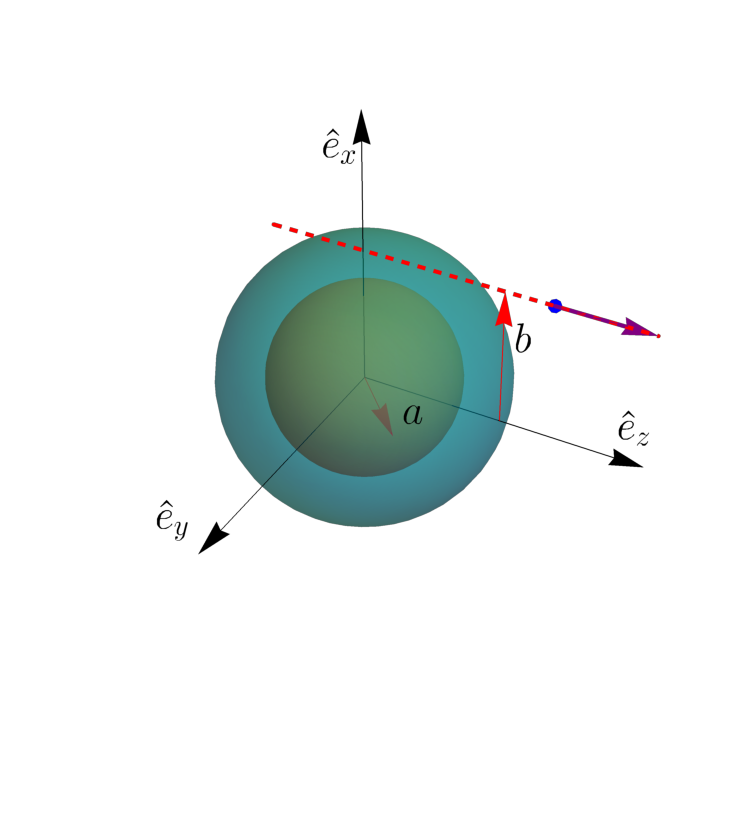
\includegraphics[width=220pt]{Figure.pdf}
\caption{Ilustración del problema; una nanopartícula esférica de radio $a$ a una distancia $b$ sobre el eje x donde pasa un electrón con velocidad $\textbf{v}$ en dirección $+z$.}
\end{figure}

\small El problema consiste en calcular el campo electromagnético debido a un electrón con velocidad relativista $\vec{v}=v\hat{e}_z$ a una distancia b del origen. Para ello se definen dos sistemas de referencia: $S$ colocado en el origen y $S'$ desde el punto de vista del electrón. Los campos de estos sistemas se relacionan mediante el tensor de Faraday 

\begin{equation}
F^{\mu\nu}=
	\begin{pmatrix}
		0					&	-\frac{E_x}{c}	&	-\frac{E_y}{c}	&	-\frac{E_z}{c}	\\
		\frac{E_x}{c}	&	0						&	-B_z					&	B_y					\\
		\frac{E_y}{c}	&	B_z					&	0						&	-B_x					\\
		\frac{E_z}{c}	&	-B_y					&	B_x					&	0						\\
	\end{pmatrix}
\label{Eq1.1}
\end{equation}

y la transformación de Lorentz

\begin{equation}
\Lambda_{\mu'}^{\mu}=
	\begin{pmatrix}
		\gamma			&	0	&	0	&	\gamma\beta	\\
		0						&	1	&	0	&	0						\\
		0						&	0	&	1	&	0						\\
		\gamma\beta	&	0	&	0	&	\gamma			\\
	\end{pmatrix},
\label{Eq1.2}
\end{equation}

del sistema $S'$ moviéndose a lo largo del eje $z$ con respecto a $S$, mediante la expresión

\begin{equation}
F^{\mu\nu}=\Lambda_{\mu'}^{\mu}\Lambda_{\nu'}^{\nu}F^{\mu'\nu'}.
\label{Eq1.3}
\end{equation}

Sustituyendo \eqref{Eq1.1} y \eqref{Eq1.2} en \eqref{Eq1.3}:

\begin{subequations}
\begin{align}
\begin{pmatrix}
		0					&	-\frac{E_x}{c}	&	-\frac{E_y}{c}	&	-\frac{E_z}{c}	\\
		\frac{E_x}{c}	&	0						&	-B_z					&	B_y					\\
		\frac{E_y}{c}	&	B_z					&	0						&	-B_x					\\
		\frac{E_z}{c}	&	-B_y					&	B_x					&	0						\\
\end{pmatrix}
&=
\begin{pmatrix}
		\gamma			&	0	&	0	&	\gamma\beta	\\
		0						&	1	&	0	&	0						\\
		0						&	0	&	1	&	0						\\
		\gamma\beta	&	0	&	0	&	\gamma			\\
\end{pmatrix}
\begin{pmatrix}
		0						&	-\frac{E_{x'}}{c}	&	-\frac{E_{y'}}{c}	&	-\frac{E_{z'}}{c}	\\
		\frac{E_{x'}}{c}	&	0						&	-B_{z'}				&	B_{y'}				\\
		\frac{E_{y'}}{c}	&	B_{z'}				&	0						&	-B_{x'}				\\
		\frac{E_{z'}}{c}	& 	-B_{y'}				&	B_{x'}				&	0						\\
\end{pmatrix}
\begin{pmatrix}
		\gamma			&	0	&	0	&	\gamma\beta	\\
		0						&	1	&	0	&	0						\\
		0						&	0	&	1	&	0						\\
		\gamma\beta	&	0	&	0	&	\gamma			\\
\end{pmatrix}	\\
&=
\begin{pmatrix}
		\gamma\beta\frac{E_{z'}}{c}	&	-\gamma\frac{E_{x'}}{c}-\gamma\beta B_{y'}	&	-\gamma\frac{E_{y'}}{c}+\gamma\beta B_{x'}	&	-\gamma\frac{E_{z'}}{c}	\\
		\frac{E_{x'}}{c}						&	0																		&	-B_{z'}																&	B_{y'}				\\
		\frac{E_{y'}}{c}						&	B_{z'}																&	0																		&	-B_{x'}				\\
		\gamma\frac{E_{z'}}{c}			& 	-\gamma\beta\frac{E_{x'}}{c}- \gamma B_{y'}	&	\gamma\beta\frac{E_{x'}}{c}+\gamma B_{x'}	&	\gamma\beta\frac{E_{z'}}{c}	\\
\end{pmatrix}
\begin{pmatrix}
		\gamma			&	0	&	0	&	\gamma\beta	\\
		0						&	1	&	0	&	0						\\
		0						&	0	&	1	&	0						\\
		\gamma\beta	&	0	&	0	&	\gamma			\\
\end{pmatrix}\\
&=
\begin{pmatrix}
		0	&	-\gamma\frac{E_{x'}}{c}-\gamma\beta B_{y'}	&	-\gamma\frac{E_{y'}}{c}+\gamma\beta B_{x'}	&	\gamma^2(\beta^2-1)\frac{E_{z'}}{c}	\\
		\gamma\frac{E_{x'}}{c}+\gamma\beta B_{y'}			&	0	&	-B_{z'}							&	\gamma\beta\frac{E_{x'}}{c}+\gamma B_{y'}					\\
		\gamma\frac{E_{y'}}{c}-\gamma\beta B_{x'}			&	B_{z'}	&	0							&	\gamma\beta\frac{E_{x'}}{c}-\gamma B_{x'}					\\
		\gamma^2(1-\beta^2)\frac{E_{z'}}{c}	& 	-\gamma\beta\frac{E_{x'}}{c}- \gamma B_{y'}	&	-\gamma\beta\frac{E_{x'}}{c}+\gamma B_{x'}	&	0	\\
\end{pmatrix}.
\end{align}
\label{Eq1.4}
\end{subequations}

De ésta última expresión se obtiene que, componente a componente, el campo desde $S$ y $S'$ se relaciona por las ecuaciones

\begin{subequations}
\begin{align}
E_x	&=\gamma (E_{x'}+c\beta B_{y'})=\gamma (E_{x'}+vB_{y'}),	\\
E_y	&=\gamma (E_{y'}-c\beta	B_{x'})=\gamma (E_{y'}-vB_{x'}),	\\
E_z	&=E_{z'},
\end{align}
\label{Eq1.5}
\end{subequations}
\begin{subequations}
\begin{align}
B_x	&=\gamma (B_{x'}-\beta\frac{E_{y'}}{c})=\gamma (B_{x'}-v\frac{E_{y'}}{c^2}),		\\
B_y	&=\gamma (B_{y'}+\beta\frac{E_{x'}}{c})=\gamma (B_{y'}+v\frac{E_{x'}}{c^2}),	\\
B_z	&=B_{z'}.
\end{align}
\label{Eq1.6}
\end{subequations}

Por la simetría del problema, el campo EM se puede separar en parte longitudinal (paralelo a la dirección del movimiento del electrón) y transversal (ortogonal a ésta)

\begin{equation}
\textbf{E}				=\textbf{E}_{\bot}+\textbf{E}_{\|}	\text{	donde	}
\textbf{E}_{\bot}	=\textbf{E}_x+\textbf{E}_y				\text{	y	}
\textbf{E}_{\|}		=\textbf{E}_z,
\label{Eq1.7}
\end{equation}
\begin{equation}
\textbf{B}				=\textbf{B}_{\bot}+\textbf{B}_{\|}	\text{	donde	}
\textbf{B}_{\bot}	=\textbf{B}_x+\textbf{B}_y				\text{	y	}
\textbf{B}_{\|}		=\textbf{B}_z.
\label{Eq1.8}
\end{equation}

Con \eqref{Eq1.7} y \eqref{Eq1.8} es posible reescribir \eqref{Eq1.5} y \eqref{Eq1.4} de la siguiente forma

\begin{subequations}
\begin{align}
\textbf{E}_{\bot}	&=\gamma(\textbf{E}_{\bot}'-\textbf{v}\times\textbf{B}'), \\
\textbf{E}_{\|}		&=\textbf{E}_{\|}',
\end{align}
\label{Eq1.9}
\end{subequations}
\begin{subequations}
\begin{align}
\textbf{B}_{\bot}	&=\gamma(\textbf{B}_{\bot}'+\textbf{v}\times\frac{\textbf{E}'}{c^2}),	\\
\textbf{B}_{\|}		&=\textbf{B}_{\|}'.
\end{align}
\label{Eq1.10}
\end{subequations}

Desde el sistema $S'$ el campo EM producido por el electrón es el de una carga puntual $q=-e$ en reposo, por lo que

\begin{subequations}
\begin{align}
\textbf{E}'		&=\frac{1}{4\pi \epsilon_0}\frac{q}{|\textbf{r} '|^2}\hat{\textbf{e}}_{r'}=\frac{q}{4\pi \epsilon_0}\frac{x'\hat{\textbf{e}}_{x'}+y'\hat{\textbf{e}}_{y'}+z'\hat{\textbf{e}}_{z'}}{[(x')^2+(y')^2+(z')^2]^{3/2}}, \\
\textbf{B}'		&=\textbf{0}.
\end{align}
\label{Eq1.11}
\end{subequations}

Sustituyendo \eqref{Eq1.15} en \eqref{Eq8} y \eqref{Eq9} se sigue que

\begin{subequations}
\begin{align}
\textbf{E}_{\bot}	&=\gamma\textbf{E}_{\bot}'=\gamma(\textbf{E}_{x'}+\textbf{E}_{y'}), \\
\textbf{E}_{\|}		&=\textbf{E}_{z'},
\end{align}
\label{Eq1.12}
\end{subequations}
\begin{subequations}
\begin{align}
\textbf{B}_{\bot}	&=\gamma\textbf{v}\times\frac{\textbf{E}'}{c^2}=\gamma\textbf{v}\times\frac{(\textbf{E}_{x'}+\textbf{E}_{y'})}{c^2},	\\
\textbf{B}_{\|}		&= \textbf{0}.
\end{align}
\label{Eq1.13}
\end{subequations}

Sin embargo, las expresiones \eqref{Eq11} y \eqref{Eq12} aún no son completas, falta hacer un cambio de las coordenadas en $S'$ por las de $S$ con la transformación

\begin{equation}
x^{\mu '}=\Lambda_{\mu}^{\mu '}x^{\mu} \text{		;		} x^{\mu}=(ct,x,y,z),
\end{equation}

obteniendo del la transformación

\begin{subequations}
\begin{align}
x'	&=	x-b,	\\
y'	&=	y,	\\
z'	&=	\gamma (z-vt),	\\
ct'	&=	\gamma (ct-\beta z),
\end{align}
\end{subequations}

se sustituye en (10) para calcular el campo eléctrico desde $S'$ con las coordenadas de $S$

\begin{equation}
\textbf{E}'(\textbf{r},t)=\frac{q}{4\pi \epsilon_0}\frac{(x-b)\hat{\textbf{e}}_x+y\hat{\textbf{e}}_y+\gamma (z-vt)\hat{\textbf{e}}_z}{[(x-b)^2+y^2+\gamma^2(z-vt)^2]^{3/2}},
\end{equation}

y a su vez (15) en (11) y (12), se obtienen los campos eléctrico y magnético

\begin{equation}
\begin{aligned}
\textbf{E}(\textbf{r};t)
	&=\frac{q\gamma}{4\pi \epsilon_0}\left\{\frac{(x-b)\hat{\textbf{e}}_x+y\hat{\textbf{e}}_y+(z-vt)\hat{\textbf{e}}_z}{[(x-b)^2+y^2+\gamma^2(z-vt)^2]^{3/2}}\right\},	\\
	&=\frac{q\gamma}{4\pi \epsilon_0}\left\{\frac{\textbf{r}-\textbf{r}_t}{[(x-b)^2+y^2+\gamma^2(z-vt)^2]^{3/2}}\right\},
\end{aligned}
\end{equation}

\begin{equation}
\begin{aligned}
\textbf{B}(\textbf{r};t)
	&=\frac{q\gamma}{4\pi \epsilon_0 c^2} \textbf{v}\times\left\{\frac{(x-b)\hat{\textbf{e}}_x+y\hat{\textbf{e}}_y}{[(x-b)^2+y^2+\gamma^2(z-vt)^2]^{3/2}}\right\},	\\
	&=\frac{\mu_0 q\gamma v}{4\pi}\left\{ \frac{-y\hat{\textbf{e}}_x+(x-b)\hat{\textbf{e}}_y}{[(x-b)^2+y^2+\gamma^2(z-vt)^2]^{3/2}}\right\}.
\end{aligned}
\end{equation}

Definiendo $R=\sqrt{(x-b)^2+y^2}$, las ecuaciones (16) y (17) pueden ser reescritas como

\begin{equation}
\textbf{E}(\textbf{r};t)	=\frac{q\gamma}{4\pi \epsilon_0}\left\{\frac{\textbf{r}-(b,0,vt)}{[R^2+\gamma^2(z-vt)^2]^{3/2}}\right\},
\end{equation}

\begin{equation}
\textbf{B}(\textbf{r};t)	=\frac{\mu_0 q\gamma v}{4\pi}\left\{ \frac{(-y,x-b,0)}{[R^{2}+\gamma^2(z-vt)^2]^{3/2}}\right\}.
\end{equation}

Por el método de obtención del campo electromagnético inducido en la NP por el campo EM del electrón, resulta necesario calcular éste último en el espacio de frecuencias $\omega$ mediante una transformada de Fourier temporal. La convención a utilizar de ésta será

\begin{equation}
\mathcal{F} (\omega)=\int_{-\infty}^{\infty} F(t)e^ {i\omega t} dt \text{		y		} F(t)=\frac{1}{2\pi}\int_{-\infty}^{\infty} \mathcal{F}(\omega)e^ {-i\omega t} d\omega,
\end{equation}

con las que se puede calcular las expresiones de las componentes de $\vec{\mathcal{E}}(\vec{r};\omega)$ y $\vec{\mathcal{B}}(\vec{r};\omega)$.
\\
Calculando la transformada de Fourier de $E_x(\vec{r};t)$:

\begin{equation}
\begin{aligned}
\mathcal{E}_x(\textbf{r};\omega)		&= \int_{-\infty}^{\infty} E_x(\textbf{r};t)e^{i\omega t} dt
					=\int_{-\infty}^{\infty} \left( \frac{q\gamma}{4\pi \epsilon_0} \right) \frac{(x-b)e^{i\omega t}}{[R^2+\gamma^2(z-vt)^2]^{3/2}} dt	\\
					&=\frac{q\gamma}{4\pi \epsilon_0} (x-b)\int_{-\infty}^{\infty} \frac{e^{i\omega t}}{[R^2+\gamma^2(z-vt)^2]^{3/2}} dt
\end{aligned}
\end{equation}

Calculando la transformada de Fourier de $E_y(\vec{r};t)$:

\begin{equation}
\begin{aligned}
\mathcal{E}_y(\textbf{r};\omega)		&= \int_{-\infty}^{\infty} E_y(\textbf{r};t)e^{i\omega t} dt
					=\int_{-\infty}^{\infty} \left( \frac{q\gamma}{4\pi \epsilon_0} \right) \frac{ye^{i\omega t}}{[R^2+\gamma^2(z-vt)^2]^{3/2}} dt	\\
					&=\frac{q\gamma}{4\pi \epsilon_0} y\int_{-\infty}^{\infty} \frac{e^{i\omega t}}{[R^2+\gamma^2(z-vt)^2]^{3/2}} dt
\end{aligned}
\end{equation}

Calculando la transformada de Fourier de $E_z(\vec{r};t)$:

\begin{equation}
\begin{aligned}
\mathcal{E}_z(\textbf{r};\omega)		&= \int_{-\infty}^{\infty} E_z(\textbf{r};t)e^{i\omega t} dt
					=\int_{-\infty}^{\infty} \left( \frac{q\gamma}{4\pi \epsilon_0} \right) \frac{(z-vt)e^{i\omega t}}{[R^2+\gamma^2(z-vt)^2]^{3/2}} dt	\\
					&=\frac{q\gamma}{4\pi \epsilon_0} \int_{-\infty}^{\infty} \frac{(z-vt)e^{i\omega t}}{[R^2+\gamma^2(z-vt)^2]^{3/2}} dt
\end{aligned}
\end{equation}

Calculando la transformada de Fourier de $B_x(\vec{r};t)$:

\begin{equation}
\begin{aligned}
\mathcal{B}_x(\textbf{r};\omega)		&= \int_{-\infty}^{\infty} B_x(\textbf{r};t)e^{i\omega t} dt
					=\int_{-\infty}^{\infty} \left( \frac{\mu_0q\gamma v}{4\pi} \right) \frac{-ye^{i\omega t}}{[R^2+\gamma^2(z-vt)^2]^{3/2}} dt	\\
					&=\frac{\mu_0q\gamma v}{4\pi}(-y)\int_{-\infty}^{\infty} \frac{e^{i\omega t}}{[R^2+\gamma^2(z-vt)^2]^{3/2}} dt
\end{aligned}
\end{equation}

Calculando la transformada de Fourier de $B_y(\vec{r};t)$:

\begin{equation}
\begin{aligned}
\mathcal{B}_y(\textbf{r};\omega)		&= \int_{-\infty}^{\infty} B_y(\textbf{r};t)e^{i\omega t} dt
					=\int_{-\infty}^{\infty} \left( \frac{\mu_0q\gamma v}{4\pi} \right) \frac{(x-b)e^{i\omega t}}{[R^2+\gamma^2(z-vt)^2]^{3/2}} dt	\\
					&=\frac{\mu_0q\gamma v}{4\pi}(x-b)\int_{-\infty}^{\infty} \frac{e^{i\omega t}}{[R^2+\gamma^2(z-vt)^2]^{3/2}} dt
\end{aligned}
\end{equation}

Como $B_z(\textbf{r};t)=0$ su tranformada de Fourier es $\mathcal{B}_z(\textbf{r};\omega)=0$.\\
En las expresiones (21-25) se frecuenta la integral 

\begin{equation}
\int_{-\infty}^{\infty} \frac{e^{i\omega t}}{[R^2+\gamma^2(z-vt)^2]^{3/2}} dt.
\end{equation}

Para resolver (26) se realiza el cambio de variable $\eta=\gamma\frac{(z-vt)}{R}$, siendo así

\begin{equation*}
\begin{aligned}
\int_{-\infty}^{\infty} \frac{e^{i\omega t}}{[R^2+\gamma^2(z-vt)^2]^{3/2}} dt &= -\frac{R}{\gamma v} \int_{-\infty}^{\infty} \frac{e^{i\omega t}}{R^3 \left[ 1+ \gamma^2 \frac{(z-vt)^2}{R^2} \right]^{3/2}} \left( -\frac{\gamma v}{R} \right) dt \\
	&= \frac{1}{\gamma vR^2} \int_{-\infty}^{\infty} \frac{e^{i\frac{\omega}{c}\left( z-\frac{R\eta}{\gamma}\right)}}{(1+\eta^2)^{3/2}} d\eta
	=\frac{e^{i\frac{\omega z}{v}} }{\gamma vR^2}\int_{-\infty}^{\infty} \frac{e^{-i\left(\frac{\omega R}{v\gamma}\right)\eta}}{(1+\eta^2)^{3/2}} d\eta.
\end{aligned}
\end{equation*}

Definiendo a la función $F_1(\alpha)$ como

\begin{equation}
F_1(\alpha)=\int_{-\infty}^{\infty} \frac{e^{-i\alpha\eta}}{(1+\eta^2)^{3/2}} d\eta,
\end{equation}

se reescribe (26) de la forma 

\begin{equation}
\int_{-\infty}^{\infty} \frac{e^{i\omega t}}{[R^2+\gamma^2(z-vt)^2]^{3/2}} dt = \frac{e^{i\frac{\omega z}{v}} }{\gamma vR^2} F_1\left( \frac{\omega R}{v\gamma}\right).
\end{equation}

Por otra parte, en (23) la integral se asemeja a (26) pero con un núcleo diferente, la cuál es

\begin{equation}
\int_{-\infty}^{\infty} \frac{(z-vt)e^{i\omega t}}{[R^2+\gamma^2(z-vt)^2]^{3/2}} dt.
\end{equation}

Realizando el mismo cambio de variable que para (26), se sigue que

\begin{equation*}
\begin{aligned}
\int_{-\infty}^{\infty} \frac{(z-vt)e^{i\omega t}}{[R^2+\gamma^2(z-vt)^2]^{3/2}} dt &= -\frac{R}{\gamma v} \int_{-\infty}^{\infty} \frac{(z-vt)e^{i\omega t}}{R^3 \left[ 1+ \gamma^2 \frac{(z-vt)^2}{R^2} \right]^{3/2}} \left( -\frac{\gamma v}{R} \right) dt \\
	&= \frac{1}{\gamma vR^2} \int_{-\infty}^{\infty} \frac{R\eta e^{i\frac{\omega}{c}\left( z-\frac{R\eta}{\gamma}\right)}}{\gamma(1+\eta^2)^{3/2}} d\eta
	=\frac{e^{i\frac{\omega z}{v}} }{\gamma^2 vR}\int_{-\infty}^{\infty} \frac{\eta e^{-i\left(\frac{\omega R}{v\gamma}\right)\eta}}{(1+\eta^2)^{3/2}} d\eta.
\end{aligned}
\end{equation*}

Definiendo a la función $F_2(\alpha)$ como

\begin{equation}
F_2(\alpha)=\int_{-\infty}^{\infty} \frac{\eta e^{-i\alpha\eta}}{(1+\eta^2)^{3/2}} d\eta,
\end{equation}

se reescribe (29) de la forma

\begin{equation}
\int_{-\infty}^{\infty} \frac{(z-vt)e^{i\omega t}}{[R^2+\gamma^2(z-vt)^2]^{3/2}} dt =\frac{e^{i\frac{\omega z}{v}} }{\gamma^2 vR} F_2\left( \frac{\omega R}{v\gamma}\right).
\end{equation}

El problema se centra en resolver las integrales con las que se definen a $F_1(\alpha)$ y $F_2(\alpha)$. Nótese que éstas son transformadas de Fourier de las funciones 

\begin{equation}
f_1(\eta)=\frac{1}{(1+\eta)^{3/2}}	\text{		y		} f_2(\eta)=\frac{\eta}{(1+\eta)^{3/2}}	 \text{      $\Rightarrow$      } f_2(\eta)=\eta f_1(\eta)
\end{equation}

respectivamente. A su vez, (32) son tales que

\begin{equation}
F_1(\alpha)=\int_{-\infty}^{\infty} f_1(\eta) e^{-i\alpha\eta} d\eta \text{		y		} F_2(\alpha)=\int_{-\infty}^{\infty} f_2(\eta) e^{-i\alpha\eta} d\eta
\end{equation}

\begin{equation}
f_1(\eta)=-\frac{1}{\eta}\frac{d}{d\eta}\left[\frac{1}{(1+\eta^2)^{1/2}}\right] \text{		y		} f_2(\eta)=-\frac{d}{d\eta}\left[\frac{1}{(1+\eta^2)^{1/2}}\right].
\end{equation}

De manera que, considerando que

\begin{equation}
\frac{d}{d\alpha}e^{-i\alpha\eta}=-i\eta e^{i\alpha\eta} \text{         $\Rightarrow$         } e^{-i\alpha\eta}=-i\int\eta e^{-i\alpha\eta}d\alpha
\end{equation}

y sustituyendo (34) en la transformada de Fourier de $f_1(\eta)$

\begin{equation*}
F_1(\alpha)	=\int_{-\infty}^{\infty} f_1(\eta) e^{-i\alpha\eta} d\eta
					=\int_{-\infty}^{\infty} f_1(\eta) \left( -i\int\eta e^{-i\alpha\eta}d\alpha\right) d\eta
					=-i \int \left( \int_{-\infty}^{\infty} \eta f_1(\eta) e^{-i\alpha\eta} d\eta \right) d\alpha
\end{equation*}

Por lo tanto
\begin{equation}
F_1(\alpha)=-i \int F_2(\alpha) d\alpha.
\end{equation}

A su vez

\begin{equation}
F_2(\alpha)	=\int_{-\infty}^{\infty} f_2(\eta) e^{-i\alpha\eta} d\eta
					=-\int_{-\infty}^{\infty} \frac{d}{d\eta}\left[\frac{1}{(1+\eta^2)^{1/2}}\right] e^{-i\alpha\eta} d\eta.
\end{equation}

Integrando por partes

\begin{equation*}
F_2(\alpha) = -\left. \frac{e^{-i\alpha\eta}}{(1+\eta^2)^{1/2}} \right|_{-\infty}^{\infty}-i\alpha \int_{-\infty}^{\infty} \frac{e^{-i\alpha\eta}}{(1+\eta^2)^{1/2}} d\eta=-i\alpha \int_{-\infty}^{\infty} \frac{e^{-i\alpha\eta}}{(1+\eta^2)^{1/2}} d\eta
\end{equation*}

De la referencia en \textsl{H. Bateman, Tables of integral transforms, (McGraw Hill Book Company, United States, 1954) Vol. 1} podemos utilizar la forma de la ecuación

\begin{equation}
\int_{-\infty}^{\infty} \frac{e^{i\frac{\nu}{\sin \eta}}}{(1+\eta^2)^{1/2}} e^{-i\alpha\eta} d\eta \overset{|\Re \{\nu\}|<1}{=} 
\left\{
\begin{aligned}
	&2e^{-\frac{1}{2}\nu \pi i}	K_{\nu}(\alpha), \alpha>0	\\
	&2e^{ \frac{1}{2}\nu \pi i}	K_{\nu}(-\alpha), \alpha<0
\end{aligned},
\right.
\end{equation}

donde $K_{\nu}(\alpha)$ es la función de Bessel modificada del segundo tipo. Considerando $\nu=0$ 

\begin{equation}
\int_{-\infty}^{\infty} \frac{e^{-i\alpha\eta}}{(1+\eta^2)^{1/2}} d\eta =
\left\{
\begin{aligned}
	&2K_{0}(\alpha), \alpha>0	\\
	&2K_{0}(-\alpha), \alpha<0
\end{aligned}
\right.
=2K_{0}(|\alpha|)
\end{equation}

Y por ello

\begin{equation}
F_2(\alpha)=-i2\alpha K_0 (|\alpha|).
\end{equation}

Sustituyendo en (36) para calcular $F_1(\alpha)$

\begin{equation}
F_1(\alpha)=-i \int (-i)2\alpha K_0 (|\alpha|) d\alpha = -2 \int \alpha K_0 (|\alpha|) d\alpha
\end{equation}

que por una relación de recursión

\begin{equation}
\int \alpha K_m (|\alpha|) d\alpha = -|\alpha| K_{m+1} (|\alpha|)
\end{equation}

Finalmente

\begin{equation}
F_1(\alpha)=2|\alpha|K_1 (|\alpha|).
\end{equation}

Siendo así, el campo electromagnético debido al electrón con velocidad $\vec{v}=v\hat{e}_z$ como función de la frecuencia $\omega$ que en términos de funciones modificadas de Bessel del segundo tipo

La componente de $E_x(\textbf{r};t)$

\begin{equation}
\begin{aligned}
\mathcal{E}_x(\textbf{r};\omega)	&=\frac{q\gamma}{4\pi\epsilon_0} (x-b)\int_{-\infty}^{\infty} \frac{e^{i\omega t}}{[R^2+\gamma^2(z-vt)^2]^{3/2}} dt	
	=\frac{q\gamma}{4\pi\epsilon_0} (x-b) \left(\frac{e^{i\frac{\omega z}{v}} }{\gamma vR^2} \right) F_1\left( \frac{\omega R}{v\gamma}\right)	\\
	&=\frac{q}{4\pi\epsilon_0} \left(\frac{x-b}{v R^2} \right) e^{i\frac{\omega z}{v}} 2 \left| \frac{\omega R}{v \gamma} \right| K_1 \left( \left| \frac{\omega R}{v \gamma} \right| \right)
	=\frac{2q}{4\pi\epsilon_0} \left(\frac{x-b}{\gamma v^2 R} \right) |\omega| e^{i\frac{\omega z}{v}} K_1 \left(\frac{|\omega| R}{v \gamma} \right)
\end{aligned}
\end{equation}

La componente de $E_y(\textbf{r};t)$

\begin{equation}
\begin{aligned}
\mathcal{E}_y(\textbf{r};\omega)	&=\frac{q\gamma}{4\pi\epsilon_0} y\int_{-\infty}^{\infty} \frac{e^{i\omega t}}{[R^2+\gamma^2(z-vt)^2]^{3/2}} dt	
	=\frac{q\gamma}{4\pi\epsilon_0} y\left(\frac{e^{i\frac{\omega z}{v}} }{\gamma vR^2} \right) F_1\left( \frac{\omega R}{v\gamma}\right)	\\
	&=\frac{q}{4\pi\epsilon_0} \left(\frac{y}{v R^2} \right) e^{i\frac{\omega z}{v}} 2 \left| \frac{\omega R}{v \gamma} \right| K_1 \left( \left| \frac{\omega R}{v \gamma} \right| \right)
	=\frac{2q}{4\pi\epsilon_0} \left(\frac{y}{\gamma v^2 R} \right) |\omega| e^{i\frac{\omega z}{v}} K_1 \left(\frac{|\omega| R}{v \gamma} \right)
\end{aligned}
\end{equation}

La componente de $E_z(\textbf{r};t)$

\begin{equation}
\begin{aligned}
\mathcal{E}_z(\textbf{r};\omega)	&=\frac{q\gamma}{4\pi\epsilon_0} \int_{-\infty}^{\infty} \frac{(z-vt)e^{i\omega t}}{[R^2+\gamma^2(z-vt)^2]^{3/2}} dt	
	=\frac{q\gamma}{4\pi\epsilon_0} \left(\frac{e^{i\frac{\omega z}{v}} }{\gamma^2 vR} \right) F_2\left( \frac{\omega R}{v\gamma}\right)	\\
	&=\frac{q}{4\pi\epsilon_0} \left(\frac{e^{i\frac{\omega z}{v}}}{\gamma v R} \right) (-2i) \frac{\omega R}{v \gamma} K_0 \left( \left| \frac{\omega R}{v \gamma} \right| \right)
	=i\frac{2q}{4\pi\epsilon_0} \left(\frac{\omega}{\gamma^2 v^2} \right) e^{i\frac{\omega z}{v}} K_0 \left(\frac{|\omega| R}{v \gamma} \right)
\end{aligned}
\end{equation}

La componente de $B_x(\textbf{r};t)$

\begin{equation}
\begin{aligned}
\mathcal{B}_x(\textbf{r};\omega)	&=\frac{\mu_0 q\gamma v}{4\pi} (-y)\int_{-\infty}^{\infty} \frac{e^{i\omega t}}{[R^2+\gamma^2(z-vt)^2]^{3/2}} dt	
	=\frac{\mu_0 q\gamma v}{4\pi} (-y) \left(\frac{e^{i\frac{\omega z}{v}} }{\gamma vR^2} \right) F_1\left( \frac{\omega R}{v\gamma}\right)	\\
	&=\frac{\mu_0 q}{4\pi} \left(\frac{-y}{R^2} \right) e^{i\frac{\omega z}{v}} 2 \left| \frac{\omega R}{v \gamma} \right| K_1 \left( \left| \frac{\omega R}{v \gamma} \right| \right)
	=\frac{2\mu_0 q}{4\pi}  \left(\frac{-y}{\gamma v R} \right) |\omega| e^{i\frac{\omega z}{v}} K_1 \left(\frac{|\omega| R}{v \gamma} \right)
\end{aligned}
\end{equation}

La componente de $B_y(\textbf{r};t)$

\begin{equation}
\begin{aligned}
\mathcal{B}_y(\textbf{r};\omega)	&=\frac{\mu_0 q\gamma v}{4\pi} (x-b)\int_{-\infty}^{\infty} \frac{e^{i\omega t}}{[R^2+\gamma^2(z-vt)^2]^{3/2}} dt	
	=\frac{\mu_0 q\gamma v}{4\pi} (x-b) \left(\frac{e^{i\frac{\omega z}{v}} }{\gamma vR^2} \right) F_1\left( \frac{\omega R}{v\gamma}\right)	\\
	&=\frac{\mu_0 q}{4\pi} \left(\frac{x-b}{R^2} \right) e^{i\frac{\omega z}{v}} 2 \left| \frac{\omega R}{v \gamma} \right| K_1 \left( \left| \frac{\omega R}{v \gamma} \right| \right)
	=\frac{2\mu_0 q}{4\pi}  \left(\frac{x-b}{\gamma v R} \right) |\omega| e^{i\frac{\omega z}{v}} K_1 \left(\frac{|\omega| R}{v \gamma} \right)
\end{aligned}
\end{equation}

Vectorialmente, el campo electromagnético del electrón toma la forma
\begin{equation}\tcboxmath[colback=cyan!5!white,colframe=cyan!75!black]{
\begin{aligned}
\textbf{E}^{\text{ext}}(\textbf{r};\omega)&= \frac{2q}{4\pi\epsilon_0} \left( \frac{\omega}{v^2 \gamma}\right) e^{i\frac{\omega z}{v}} \left\{ \left[\frac{sgn(\omega)}{R}K_1 \left(\frac{|\omega| R}{v \gamma} \right) \right] [(x-b)\hat{\textbf{e}}_x+y\hat{\textbf{e}}_y]-\frac{i}{\gamma} K_0 \left(\frac{|\omega| R}{v \gamma} \right) \hat{\textbf{e}}_z \right\}	\\
\textbf{B}^{\text{ext}}(\textbf{r};\omega)&= \frac{2\mu_0 q}{4\pi} \left( \frac{|\omega|}{v\gamma R} \right) e^{i\frac{\omega z}{v}} K_1 \left(\frac{|\omega| R}{v \gamma} \right) [-y\hat{\textbf{e}}_x +(x-b)\hat{\textbf{e}}_y]
\end{aligned}}
\end{equation}

Las gráficas corresponientes a éstas expresiones se presentan en la Fig. 2

\begin{figure}[htbp]
\begin{subfigure}[b]{0.5\textwidth}
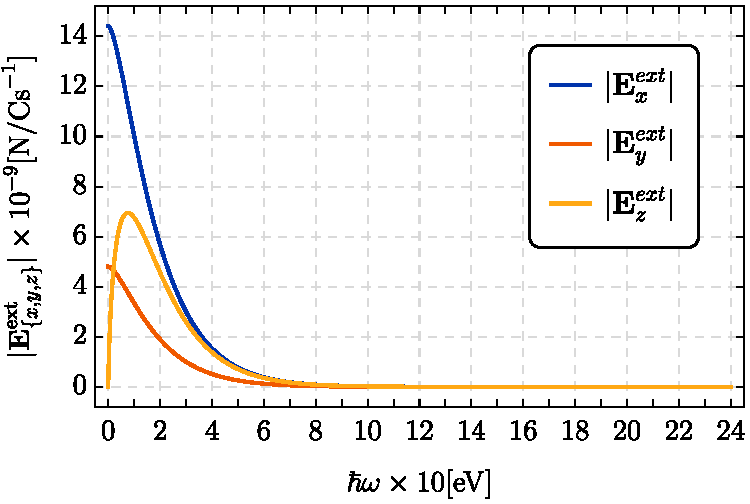
\includegraphics[width=220pt]{EextGraph2.pdf}
\caption{}
\end{subfigure}
\begin{subfigure}[b]{0.5\textwidth}
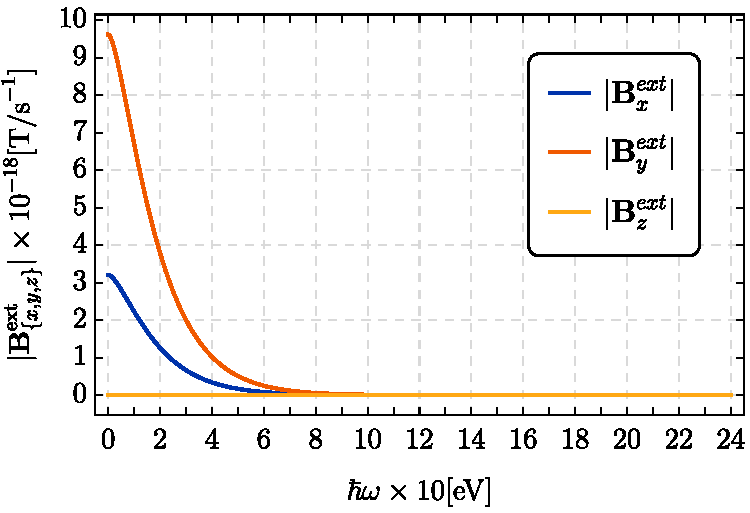
\includegraphics[width=220pt]{BextGraph2.pdf}
\caption{}
\end{subfigure}
\begin{subfigure}[b]{0.5\textwidth}
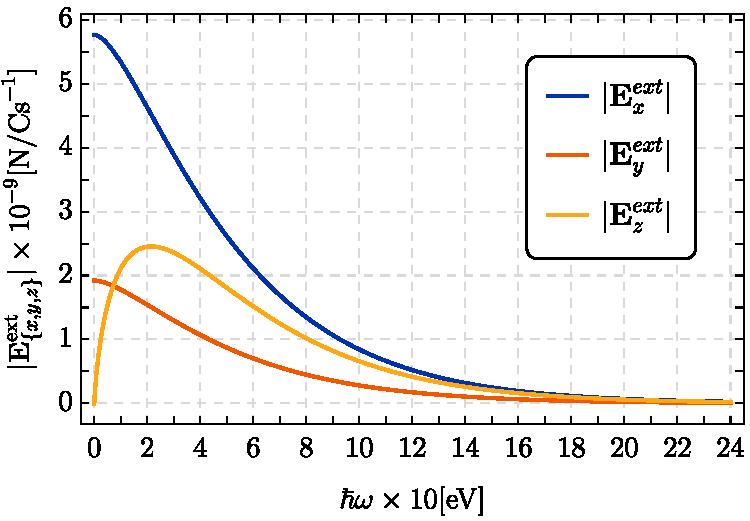
\includegraphics[width=220pt]{EextGraph.pdf}
\caption{}
\end{subfigure}
\begin{subfigure}[b]{0.5\textwidth}
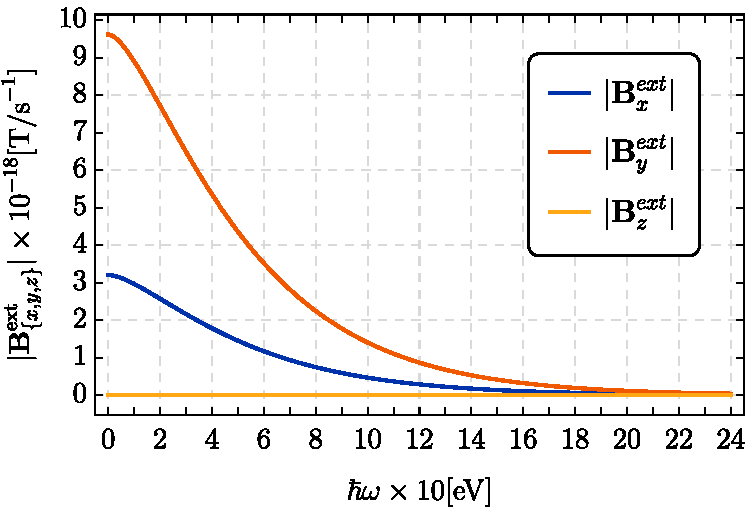
\includegraphics[width=220pt]{BextGraph.pdf}
\caption{}
\end{subfigure}
\begin{subfigure}[b]{0.5\textwidth}
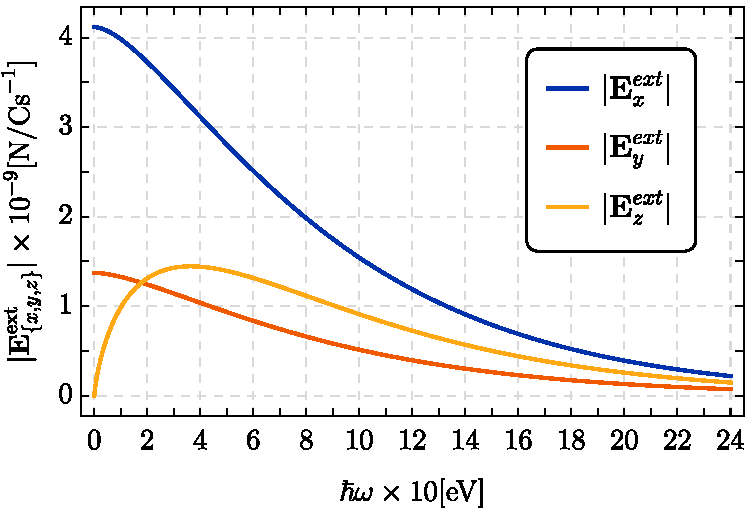
\includegraphics[width=220pt]{EextGraph7.pdf}
\caption{}
\end{subfigure}
\begin{subfigure}[b]{0.5\textwidth}
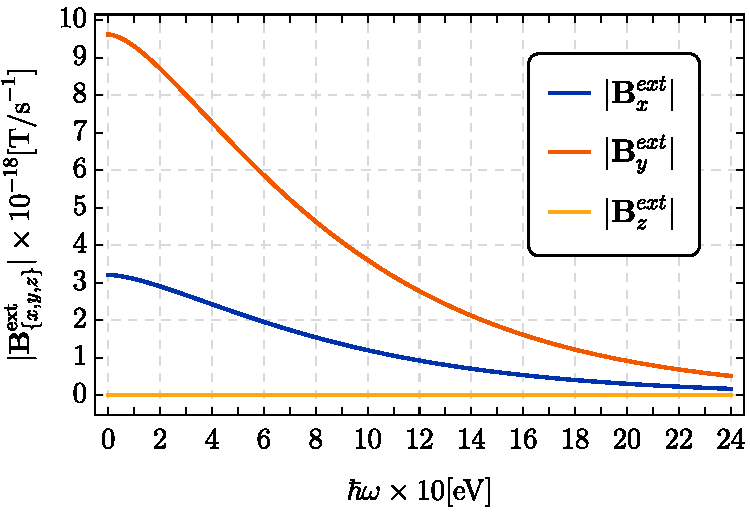
\includegraphics[width=220pt]{BextGraph7.pdf}
\caption{}
\end{subfigure}
\caption{Gráficas de la magnitud de las componentes del (a) campo eléctrico y (b) campo magnético producido por un electrón con velocidad $\textbf{v}=$(0.2$c)\hatbf{e}_z$ y parámetro de impacto $b$=3 nm como función de la energía $\hbar\omega$. Ambos campos son evaluados en el punto $\textbf{r}=(0,-1,0)$. }
\end{figure}

\section{\large{Cálculo del potenical eléctrico debido a un electrón en movimiento rectilíneo uniforme: expansión multipolar}}

\setcounter{equation}{0}

Otra manera de obtener el campo electromagnético es mediante las ecuaciones de Maxwell

\begin{subequations}
\begin{align}
\nabla\cdot\textbf{D}(\textbf{r};t)	&=\rho_{ext}(\textbf{r};t),	\label{GaussE}	\\
\nabla\cdot\textbf{B}(\textbf{r};t)	&=0,		\label{GaussM}	\\
\nabla\times\textbf{E}(\textbf{r};t)	&= -\frac{\partial}{\partial t}\textbf{B}(\textbf{r};t),	\label{FaradayLenz}	\\
\nabla\times\textbf{H}(\textbf{r};t)	&=\textbf{J}_{ext}(\textbf{r};t)+\frac{\partial}{\partial t}\textbf{D}(\textbf{r};t).	\label{AmpereMaxwell}
\end{align}
\label{EcsMaxwell}
\end{subequations}

De \eqref{GaussM} y \eqref{FaradayLenz} se pueden definir los potenciales $\phi(\vec{r};t)$ y $\vec{A}(\vec{r};t)$ tales que

\begin{subequations}
\begin{align}
\textbf{E}(\textbf{r};t)	&=-\nabla\phi(\textbf{r};t) -\frac{\partial}{\partial t}\textbf{A}(\textbf{r};t),	\\
\textbf{B}(\textbf{r};t)	&=\nabla\times\textbf{A}(\textbf{r};t).
\end{align}
\label{PotencialesReales}
\end{subequations}

Calculando las transformaciones de Fourier temporales de \eqref{GaussE},\eqref{AmpereMaxwell} y \eqref{PotencialesReales}

\begin{subequations}
\begin{align}
\nabla\cdot\textbf{D}(\textbf{r};\omega)	&=\mathcal{\rho}_{ext}(\textbf{r};\omega),	\\
\nabla\times\textbf{H}(\textbf{r};\omega)	&=\textbf{J}_{ext}(\textbf{r};\omega)-i\omega\textbf{D}(\textbf{r};\omega),
\end{align}
\label{Eq2.3}
\end{subequations}
\begin{subequations}
\begin{align}
\textbf{E}(\textbf{r};\omega)	&= -\nabla\phi(\textbf{r};\omega) +i\omega\textbf{A}(\textbf{r};\omega),	\\
\textbf{B}(\textbf{r};\omega)	&=\nabla\times\textbf{A}(\textbf{r};\omega).
\end{align}
\label{Eq2.4}
\end{subequations}

Pensando que el electrón se mueve en un medio simple (lineal, homogéneo e isótropo), podemos hacer uso de las relaciones

\begin{subequations}
\begin{align}
\textbf{D}(\textbf{r};\omega)=\epsilon(\omega)\textbf{E}(\textbf{r};\omega),	\\
\textbf{B}(\textbf{r};\omega)=\mu(\omega)\textbf{H}(\textbf{r};\omega),
\end{align}
y de la definción de índice refracción
\begin{equation}
n^2(\omega)=\mu_r (\omega) \epsilon_r (\omega)= \frac{\mu(\omega)}{\mu_0} \frac{\epsilon(\omega)}{\epsilon_0}=\mu(\omega)\epsilon(\omega)c^2
\end{equation}
\label{lineal}
\end{subequations}

que sustituyendo \eqref{PotOme} y \eqref{lineal} en \eqref{MaxOme}

\begin{subequations}
\begin{align}
\nabla\cdot\textbf{D} (\textbf{r};\omega)	&=	\rho_{ext}(\textbf{r},\omega)\\
\nabla\cdot[\epsilon(\omega)\textbf{E}(\textbf{r};\omega)]	&=	\rho_{ext}(\textbf{r},\omega)\\
\nabla\cdot[-\nabla\phi(\textbf{r};\omega)+i\omega\textbf{A}(\textbf{r};\omega)]	&=	\frac{\rho_{ext}(\textbf{r};\omega)}{\epsilon(\omega)}	\\
-\nabla^2\phi(\textbf{r};\omega)+i\omega\nabla\cdot\textbf{A}(\textbf{r};\omega)	&=	\frac{\rho_{ext}(\textbf{r};\omega)}{\epsilon(\omega)}
\end{align}
\label{1max}
\end{subequations}

\begin{subequations}
\begin{align}
\nabla\times\textbf{H}(\textbf{r};\omega)	&=\textbf{J}_{ext}(\textbf{r};\omega)-i\omega\textbf{D}(\textbf{r};\omega) \\
\nabla\times\left[\frac{\textbf{B}(\textbf{r};\omega)}{\mu(\omega)} \right]	&= \textbf{J}_{ext}(\textbf{r};\omega)-i\omega\epsilon(\omega)\textbf{E}(\textbf{r};\omega)	\\
\nabla\times[\nabla\times\textbf{A}(\textbf{r};\omega)]	&= \mu(\omega)\textbf{J}_{ext}(\textbf{r};\omega)-i\omega\mu(\omega)\epsilon(\omega)[-\nabla\phi(\textbf{r};\omega)+i\omega\textbf{A}(\textbf{r};\omega)]	\\
\nabla[\nabla\cdot\textbf{A}(\textbf{r};\omega)]-\nabla^2\textbf{A}(\textbf{r};\omega) &= \mu(\omega)\textbf{J}_{ext}(\textbf{r};\omega)+\nabla[i\omega\frac{n^2(\omega)}{c^2}\phi(\textbf{r};\omega)]+\omega^2\frac{n^2(\omega)}{c^2}\textbf{A}(\textbf{r};\omega)	\\
\nabla^2\textbf{A}(\textbf{r};\omega) +\omega^2\frac{n^2(\omega)}{c^2}\textbf{A}(\textbf{r};\omega)	&=-\mu(\omega)\textbf{J}_{ext}(\textbf{r};\omega)+\nabla[\nabla\cdot\textbf{A}(\textbf{r};\omega)-i\omega\frac{n^2(\omega)}{c^2}\phi(\textbf{r};\omega)].
\end{align}
\label{2max}
\end{subequations}

Siendo la norma de Lorenz en medios simples

\begin{equation}
\nabla\cdot\textbf{A}(\textbf{r};t)+\frac{n^2}{c^2}\frac{\partial}{\partial t}\phi(\textbf{r};t)=0,
\end{equation}

su transformada de Fourier temporal es

\begin{equation}
\nabla\cdot\textbf{A}(\textbf{r};\omega)-i\omega\frac{n^2(\omega)}{c^2}\phi(\textbf{r};\omega)=0.
\label{NormOme}
\end{equation}

Sustituyendo \eqref{NormOme} en las últimas expresiones de \eqref{1max} y \eqref{2max}, se obtiene

\begin{subequations}
\begin{align}
\left[ \nabla^2+\omega^2\frac{n^2(\omega)}{c^2}\right] \phi(\textbf{r};\omega) &=-\frac{\rho_{ext}(\textbf{r};\omega)}{\epsilon(\omega)}	\label{59a}	\\
\left[ \nabla^2+\omega^2\frac{n^2(\omega)}{c^2}\right]\textbf{A}(\textbf{r};\omega) &=-\mu(\omega)\textbf{J}_{ext}(\textbf{r};\omega).
\end{align}
\label{PotOmeg}
\end{subequations}

Calculando las transformadas de Fourier espaciales, definidas por

\begin{subequations}
\begin{align}
\mathcal{F} (\textbf{k})=\int_{-\infty}^{\infty} F(\textbf{r})e^ {-i\textbf{k}\cdot\textbf{r}} d^3r,
F(\textbf{r})=\frac{1}{2\pi}\int_{-\infty}^{\infty} \mathcal{F}(\textbf{k})e^ {i\textbf{k}\cdot\textbf{r}} d^3k,
\end{align}
\end{subequations}

de \eqref{PotOmeg} se tienen

\begin{subequations}
\begin{align}
\left[ -k^2+\omega^2\frac{n^2(\omega)}{c^2}\right] \phi(\textbf{k};\omega)&=-\frac{\rho_{ext}(\textbf{k};\omega)}{\epsilon(\omega)},	\\
\left[ -k^2+\omega^2\frac{n^2(\omega)}{c^2}\right]\textbf{A}(\textbf{k};\omega)&=-\mu(\omega)\textbf{J}_{ext}(\textbf{k};\omega).
\end{align}
\label{PotOmeK}
\end{subequations}

Notando que la única fuente de carga externa es la del electrón en movimiento, las densidades de carga y corriente son

\begin{subequations}
\begin{align}
\rho_{ext}(\textbf{r};t)&=q\delta(\textbf{r}-\textbf{r}_t)	\label{Eq2.13a}	\\
\textbf{J}_{ext}(\textbf{r};t)&=\rho_{ext}(\textbf{r};t) \textbf{v}	\label{Eq2.13b}
\end{align}
\label{densidadesreales}
\end{subequations}

donde \eqref{corrientereal} se cumple también en el espacio $(\textbf{k};\omega)$, de modo que \eqref{PotOmeK} se reecribe como

\begin{subequations}
\begin{align}
\phi(\textbf{k};\omega)=-\frac{\rho_{ext}(\textbf{k};\omega)}{\epsilon(\omega)\left[ -k^2+\omega^2\frac{n^2(\omega)}{c^2}\right] },	\label{Pot3}	\\
\textbf{A}(\textbf{k};\omega)=-\frac{\mu(\omega)\rho_{ext}(\textbf{r};t) \textbf{v}}{\left[ -k^2+\omega^2\frac{n^2(\omega)}{c^2}\right]},
\end{align}
\label{Pot2}
\end{subequations}

de donde se sigue que

\begin{equation}
\textbf{A}(\textbf{k};\omega)=\mu(\omega)\epsilon(\omega)\textbf{v}\phi(\textbf{k};\omega)=\frac{n^2(\omega)}{c^2}\textbf{v}\phi(\textbf{k};\omega)
\label{Pot5}
\end{equation}

o bien, haciendo la transformada inversa de Fourier espacial de \eqref{Pot5}

\begin{equation}
\textbf{A}(\textbf{r};\omega)=\frac{n^2(\omega)}{c^2}\textbf{v}\phi(\textbf{r};\omega)
\end{equation}

sustituyendo en \eqref{PotOme} se concluye que

\begin{subequations}
\begin{align}
\textbf{E}^{ext}(\textbf{r};\omega)&=\left[-\nabla+i\omega\frac{n^2(\omega)}{c^2}\textbf{v} \right] \phi^{ext}(\textbf{r};\omega)	\label{Eq2.17a}\\
\textbf{B}^{ext}(\textbf{r};\omega)&=\frac{n^2(\omega)}{c^2}\nabla\times[\textbf{v}\phi^{ext}(\textbf{r};\omega)]
\end{align}
\end{subequations}

donde el super índice $ext$ refiere al carácter externo del campo EM producido por el electrón, una carga externa. \\ 
Para calcular $\phi^{ext}(\textbf{r};\omega)$ se realiza una transformada inversa de Fourier espacial de \eqref{Pot3}. A su vez, para resolver ésta se tendrá que calcular $\rho_{ext}(\textbf{k};\omega)$ con una transformada de Fourier temporal y espacial de \eqref{cargareal}. Así

\begin{equation}
\begin{aligned}
\rho_{ext} (\textbf{k};\omega)	&=\int_{V} \int_{-\infty}^{\infty} \rho_{ext} (\textbf{r};t) e^{-i(\textbf{k}\cdot\textbf{r}-\omega t)} dt d^3r
	=q\int_{-\infty}^{\infty} \int_{V}\delta(\textbf{r}-\textbf{r}_t)  e^{-i(\textbf{k}\cdot\textbf{r}-\omega t)} d^3r dt	\\
&=q\int_{-\infty}^{\infty}  e^{-i(\textbf{k}\cdot\textbf{r}_t-\omega t)} dt	
	=	q e^{-i\textbf{k}\cdot\textbf{r}_0}\int_{-\infty}^{\infty}e^{-i(\textbf{k}\cdot\textbf{v}-\omega )t} dt\\
&=2\pi q e^{-i\textbf{k}\cdot\textbf{r}_0}\delta(\textbf{k}\cdot\textbf{v}-\omega).
\end{aligned}
\label{68}
\end{equation}

Sustituyendo \eqref{68} en \eqref{Pot3}

\begin{equation}
\phi^{ext}(\textbf{k};\omega)=\frac{2\pi qe^{-i\textbf{k}\cdot\textbf{r}_0}\delta(\textbf{k}\cdot\textbf{v}-\omega)}{\epsilon(\omega)\left[ k^2-\frac{\omega^2}{c^2}n^2(\omega) \right]}
\label{philome}
\end{equation}

y calculando la transformada de Fourier inversa espacial de \eqref{philome}

\begin{subequations}
\begin{equation}
\begin{aligned}
\phi^{ext}(\textbf{r};\omega)	&=	\frac{1}{(2\pi)^3} \int_{V_{k}} \phi^{ext}(\textbf{k};\omega) e^{i\textbf{k}\cdot\textbf{r}} d^3k
	=\frac{1}{(2\pi)^3} \int_{V_{k}} \frac{2\pi qe^{-i\textbf{k}\cdot\textbf{r}_0}\delta(\textbf{k}\cdot\textbf{v}-\omega)}{\epsilon(\omega)\left[ k^2-\frac{\omega^2}{c^2}n^2(\omega) \right]} e^{i\textbf{k}\cdot\textbf{r}} d^3k	\\
	&= \frac{q}{(2\pi)^2\epsilon(\omega)} \int_{V_k} \frac{\delta(\textbf{k}\cdot\textbf{v}-\omega)e^{-i(\textbf{k}\cdot\textbf{r}_0-\textbf{k}\cdot\textbf{r})}}{k^2-\frac{\omega^2}{c^2}n^2(\omega)} d^3 k,
\end{aligned}
\end{equation}
donde $\textbf{k}=(k_x,k_y,k_z)$,$\textbf{v}=v\hat{\textbf{e}}_z$ y $\textbf{r}_0=b\hat{\textbf{e}}_x$. Entonces
\begin{equation}
\begin{aligned}
\phi^{ext}(\textbf{r};\omega)	
	&=\frac{q}{(2\pi)^2\epsilon(\omega)}\int_{-\infty}^{\infty}\int_{-\infty}^{\infty}\int_{-\infty}^{\infty} \frac{\delta(k_zv-\omega)e^{i[k_x(x-b)+k_yy+k_zz]}}{k_x^2+k_y^2+k_z^2-\frac{\omega^2}{c^2}n^2(\omega)} dk_z dk_y dk_x \\
	&=\frac{q}{(2\pi)^2v\epsilon(\omega)}\int_{-\infty}^{\infty}e^{ik_x(x-b)}\int_{-\infty}^{\infty}e^{ik_yy}\int_{-\infty}^{\infty}\frac{\delta(k_z-\frac{\omega}{v})e^{ik_zz}}{k_x^2+k_y^2+k_z^2-\frac{\omega^2}{c^"}n^2(\omega)}dk_z dk_y dk_x	\\
	&=\frac{q}{(2\pi)^2v\epsilon(\omega)}\int_{-\infty}^{\infty}e^{ik_yy}\int_{-\infty}^{\infty}e^{ik_x(x-b)}\frac{e^{i\frac{\omega z}{v}}}{k_x^2+k_y^2+\frac{\omega^2}{v^2}-\frac{\omega^2}{c^2}n^2(\omega)} dk_x dk_y	\\
	&=\frac{qe^{i\frac{\omega z}{v}}}{(2\pi)^2v\epsilon(\omega)}\int_{-\infty}^{\infty}e^{ik_yy}\int_{-\infty}^{\infty} \frac{e^{ik_x(x-b)}}{k_x^2+k_y^2+\frac{\omega^2}{v^2}\left[1-\frac{v^2}{c^2}n^2(\omega) \right]} dk_x dk_y
\end{aligned}
\end{equation}
definiendo 
\begin{equation}
\gamma_n(\omega)=\frac{1}{\sqrt{1-	\frac{v^2}{c^2}n^2(\omega)}}
\end{equation}
y sustituyendo
\begin{equation}
\begin{aligned}
\phi^{ext}(\textbf{r};\omega)
	&=\frac{qe^{i\frac{\omega z}{v}}}{(2\pi)^2v\epsilon(\omega)}\int_{-\infty}^{\infty}e^{ik_yy}\int_{-\infty}^{\infty} \frac{e^{ik_x(x-b)}}{k_x^2+k_y^2+\frac{\omega^2}{v^2\gamma_n^2(\omega)}} dk_x dk_y
\end{aligned}
\end{equation}
Haciendo uso de la simetría cilíndrica del problema, como se debe cumplir para todo $(x,y)$ tales que $(x-b)^2+y^2=R^2$ lo hace en particular para $x=b$ y $y=R$. Siendo así
\begin{equation}
\begin{aligned}
\phi^{ext}(\textbf{r};\omega)
	&=\frac{qe^{i\frac{\omega z}{v}}}{(2\pi)^2v\epsilon(\omega)}\int_{-\infty}^{\infty}e^{ik_yR}\int_{-\infty}^{\infty} \frac{dk_x}{k_x^2+\left[ k_y^2+\frac{\omega^2}{v^2\gamma_n^2(\omega)}\right]} dk_y.
\end{aligned}
\label{70e}
\end{equation}

Recordando que

\begin{equation}
\int_{-\infty}^{\infty}\frac{dk}{k^2+a^2}=\frac{1}{|a|}\arctan(\theta)\arrowvert_{-\frac{\pi}{2}}^{\frac{\pi}{2}}=\frac{\pi}{a},
\end{equation}

se sustituye en \eqref{70e}, donde $\xi=\frac{\omega}{v\gamma_n}$

\begin{equation}
\begin{aligned}
\phi^{ext}(\textbf{r};\omega)
	&=\frac{qe^{i\frac{\omega z}{v}}}{4\pi^2 v\epsilon(\omega)}\int_{-\infty}^{\infty}\frac{\pi e^{iR}}{\sqrt{k_y^2+\frac{\omega^2}{v^2\gamma_n^2(\omega)}}} dk_y
	=\frac{qe^{i\frac{\omega z}{v}}}{4\pi v\epsilon(\omega)}\int_{-\infty}^{\infty} \frac{e^{ik_yR}}{\sqrt{k_y^2+\xi^2}} dk_y	\\
	&=\frac{qe^{i\frac{\omega z}{v}}}{4\pi v\epsilon(\omega)}\int_{-\infty}^{\infty} \frac{e^{ik_yR}}{\sqrt{1+(\frac{k_y}{\xi})^2}}\left(\frac{1}{\xi}\right) dk_y
\end{aligned}
\end{equation}

Haciendo el cambio de variable $\eta=\frac{k_y}{\xi}$

\begin{equation}
\begin{aligned}
\phi^{ext}(\textbf{r};\omega)
	&=\frac{qe^{i\frac{\omega z}{v}}}{4\pi v\epsilon(\omega)}\int_{-\infty}^{\infty}\frac{e^{i(\xi\eta)R}}{\sqrt{1+\eta^2}} d\eta
	=\frac{qe^{i\frac{\omega z}{v}}}{4\pi v\epsilon(\omega)}\int_{-\infty}^{\infty}\frac{e^{i(\xi R)\eta}}{\sqrt{1+\eta^2}} d\eta
	=\frac{qe^{i\frac{\omega z}{v}}}{4\pi v\epsilon(\omega)}F_1(\xi R)	\\
	&=\frac{qe^{i\frac{\omega z}{v}}}{4\pi v\epsilon(\omega)} 2K_0(|\xi R|)
\end{aligned}
\end{equation}
\end{subequations}

Por lo tanto
\begin{equation}
\tcboxmath[colback=cyan!5!white,colframe=cyan!75!black]{
\phi^{ext}(\textbf{r};\omega)=\frac{1}{4\pi\epsilon(\omega)}\frac{2q}{v}e^{i\frac{\omega z}{v}}K_0\left( \frac{|\omega|R}{v\gamma_n} \right).}
\label{PotencialExt1}
\end{equation}

Por otra parte, resolviendo por el método de la función de Green la ecuación \eqref{59a} partiendo de

\begin{subequations}
\begin{equation}
(\nabla'^2+k^2)\phi(\textbf{r}';\omega)=-	\frac{\rho_{ext}(\textbf{r}';\omega)}{\epsilon(\omega)}
\label{71a}
\end{equation}
\begin{equation}
(\nabla'^2+k^2)G(\textbf{r},\textbf{r}')=-\delta(\textbf{r}-\textbf{r}')
\label{71b}
\end{equation}
\end{subequations}

Multiplicando \eqref{71a} por $G(\textbf{r},\textbf{r}')$ y \eqref{71b} por $\phi(\textbf{r}';\omega)$

\begin{subequations}
\begin{equation}
G(\textbf{r},\textbf{r}')\nabla'^2\phi(\textbf{r}';\omega)+G(\textbf{r},\textbf{r}')k^2\phi(\textbf{r}';\omega)=-G(\textbf{r},\textbf{r}')\frac{\rho_{ext}(\textbf{r}';\omega)}{\epsilon(\omega)}
\label{72a}
\end{equation}
\begin{equation}
\phi(\textbf{r}';\omega)\nabla'^2G(\textbf{r},\textbf{r}')+\phi(\textbf{r}';\omega)k^2G(\textbf{r},\textbf{r}')=-\phi(\textbf{r}';\omega)\delta(\textbf{r}-\textbf{r}')
\label{72b}
\end{equation}
\end{subequations}

Restando \eqref{72b} a \eqref{72a} e integrando en todo el espacio $V'$

\begin{equation*}
\begin{aligned}
G(\textbf{r},\textbf{r}')\nabla'^2\phi(\textbf{r}';\omega)-\phi(\textbf{r}';\omega)\nabla'^2G(\textbf{r},\textbf{r}')	&=	\phi(\textbf{r}';\omega)\delta(\textbf{r}-\textbf{r}')-G(\textbf{r},\textbf{r}')\frac{\rho_{ext}(\textbf{r}';\omega)}{\epsilon(\omega)}	\\
\int_{V'} G(\textbf{r},\textbf{r}')\nabla'^2\phi(\textbf{r}';\omega)-\phi(\textbf{r}';\omega)\nabla'^2G(\textbf{r},\textbf{r}') d^3r'	&=	\int_{V'}\phi(\textbf{r}';\omega)\delta(\textbf{r}-\textbf{r}')-G(\textbf{r},\textbf{r}')\frac{\rho_{ext}(\textbf{r}';\omega)}{\epsilon(\omega)} d^3r'	\\
\oint_{S'} [G(\textbf{r},\textbf{r}')\nabla'\phi(\textbf{r}';\omega)-\phi(\textbf{r}';\omega)\nabla'G(\textbf{r},\textbf{r}')]\cdot d\textbf{a}		&=	\int_{V'}\phi(\textbf{r}';\omega)\delta(\textbf{r}-\textbf{r}') d^3r'-\int_{V'}G(\textbf{r},\textbf{r}')\frac{\rho_{ext}(\textbf{r}';\omega)}{\epsilon(\omega)} d^3r'	\\
0	&=	\phi(\textbf{r};\omega)-\frac{1}{\epsilon(\omega)}\int_{V'} \rho_{ext}(\textbf{r}';\omega) G(\textbf{r};\textbf{r}') d^3r'	\\
\phi(\textbf{r};\omega)	&=	\frac{1}{\epsilon(\omega)}\int_{V'} \rho_{ext}(\textbf{r}';\omega) G(\textbf{r};\textbf{r}') d^3r'
\end{aligned}
\end{equation*}

donde

\begin{equation}
\rho_{ext}(\textbf{r}';\omega)=\int_{-\infty}^{\infty}\rho_{ext}(\textbf{r}';t) e^{i\omega t} dt = q\int_{-\infty}^{\infty} \delta(\textbf{r}'-\textbf{r}_t)e^{i\omega t} dt
\end{equation}

siguiendo que
\begin{subequations}
\begin{equation}
\begin{aligned}
\phi(\textbf{r};\omega)	&=	\frac{1}{\epsilon(\omega)}\int_{V'} \left( q\int_{-\infty}^{\infty} \delta(\textbf{r}'-\textbf{r}_t)e^{i\omega t} dt \right) G(\textbf{r};\textbf{r}') d^3r'	\\	&=	\frac{q}{\epsilon(\omega)}\int_{-\infty}^{\infty}e^{i\omega t} \int_{V'} \delta(\textbf{r}'-\textbf{r}_t)G(\textbf{r};\textbf{r}')d^3r' dt
\end{aligned}
\end{equation}
por tanto
\begin{equation}
\phi^{ext}(\textbf{r};\omega) =	\frac{q}{\epsilon(\omega)}\int_{-\infty}^{\infty} G(\textbf{r};\textbf{r}_t) e^{i\omega t}dt
\label{Eq2.25b}
\end{equation}
\end{subequations}

donde $G(\textbf{r};\textbf{r}_t)$ es la ecuación de Green de la ecuación de Helmholtz dada por

\begin{equation}
G(\textbf{r};\textbf{r}_t)=\frac{e^{ik|\textbf{r}-\textbf{r}_t|}}{4\pi|\textbf{r}-\textbf{r}_t|}.
\end{equation}

Como se busca una expasión multipolar del campo EM del electrón, resulta conveniente utilizar la expasión de la función de Green dada por el Teorema de Adición, siendo así (Jackson pag. 428)

\begin{equation}
G(\textbf{r};\textbf{r}_t)=k\sum_{l=1}^{\infty}\sum_{m=-l}^{l} j_l(kr_{<})h_l^{(+)}(kr_{>})Y_l^{m*}(\theta_t,\varphi_t)Y_l^m(\theta,\varphi)
\label{ExpansionGreen}
\end{equation}

donde 

\begin{equation}
r_{<}=
\left\{
\begin{aligned}
	r_t, r_t<r	\\
	r, r<r_t
\end{aligned}
\right.
\textbf{	y	}
r_{>}=
\left\{
\begin{aligned}
	r_t, r_t>r	\\
	r, r>r_t
\end{aligned}
\right.,
\end{equation}

$j_l(\rho)$ es una función esférica de Bessel, $h_l^{(+)}(\rho)$ una función esférica de Hankel del primer tipo multiplicada por $i$, $Y_l^m(\theta,\varphi)$ un armónico esférico definido por

\begin{equation}
Y_l^m(\theta,\varphi)=a_{l,m}P_l^m(\cos\theta)e^{im\varphi}=\sqrt{\frac{2l+1}{4\pi}\frac{(l-m)!}{(l+m)!}}P_l^m(\cos\theta)e^{im\varphi}
\end{equation}

donde a su vez $P_l^m(\nu)$ es una función asociada de Legendre. Sustituyendo \eqref{ExpansionGreen} en \eqref{PotencialExt2} y considerando que $r_t>r$

\begin{equation}
\begin{aligned}
\phi^{ext}(\textbf{r};\omega)	&=\frac{1}{\epsilon(\omega)}\int_{-\infty}^{\infty} e^{i\omega t} G(\vec{r};\vec{r}_t)dt=\frac{q}{\epsilon(\omega)}\int_{-\infty}^{\infty} e^{i\omega t} k\sum_{l=1}^{\infty}\sum_{m=-l}^{l} j_l(kr)h_l^{(+)}(kr_t)Y_l^{m*}(\theta_t,\varphi_t)Y_l^m(\theta,\varphi) dt	\\
	&=\frac{qk}{\epsilon(\omega)}\sum_{l=1}^{\infty}\sum_{m=-l}^l j_l(kr)Y_l^m(\theta,\varphi)\int_{-\infty}^{\infty}e^{i\omega t} h_l^{(+)}(kr_t)Y_l^{m*}(\theta_t,\varphi_t) dt	\\
	&=\frac{qk}{\epsilon(\omega)}\sum_{l=1}^{\infty}\sum_{m=-l}^l j_l(kr)Y_l^m(\theta,\varphi) M_{l,m}^{(+)},
\end{aligned}
\label{PotencialExt3}
\end{equation}

definiendo 

\begin{equation}
M_{l,m}^{(+)}=\int_{-\infty}^{\infty}e^{i\omega t} h_l^{(+)}(kr_t)Y_l^{m*}(\theta_t,\varphi_t) dt.
\label{Mlm}
\end{equation}

Para resolver \eqref{Mlm} igualamos la última expresión de \eqref{PotencialExt3} con \eqref{PotencialExt1}

\begin{equation}
\begin{aligned}
\frac{1}{4\pi\epsilon(\omega)}\frac{2q}{v}e^{i\frac{\omega z}{v}}K_0\left( \frac{|\omega|R}{v\gamma_n} \right)	&=	\frac{qk}{\epsilon(\omega)}\sum_{l=1}^{\infty}\sum_{m=-l}^l j_l(kr)Y_l^m(\theta,\varphi) M_{l,m}^{(+)}	\\
\frac{e^{i\frac{\omega z}{v}}}{2\pi kv}K_0\left( \frac{|\omega|R}{v\gamma_n} \right)	&=	\sum_{l=1}^{\infty}\sum_{m=-l}^l j_l(kr)Y_l^m(\Omega) M_{l,m}^{(+)}	\\
\int_{0}^{4\pi}\frac{e^{i\frac{\omega z}{v}}}{2\pi kv}K_0\left( \frac{|\omega|R}{v\gamma_n} \right) Y_{l'}^{m'*}(\Omega) d\Omega		&=	\int_{0}^{4\pi} \sum_{l=1}^{\infty}\sum_{m=-l}^l j_l(kr)Y_l^m(\Omega)  Y_{l'}^{m'*}(\Omega)  M_{l,m}^{(+)} d\Omega	\\
\frac{1}{2\pi kv}\int_{0}^{4\pi}e^{i\frac{\omega z}{v}}K_0\left( \frac{|\omega|R}{v\gamma_n} \right) Y_{l'}^{m'*}(\Omega) d\Omega	&=	\sum_{l=1}^{\infty}\sum_{m=-l}^l j_l(kr)M_{l,m}^{(+)} \int_{0}^{4\pi} Y_l^m(\Omega)  Y_{l'}^{m'*}(\Omega) d\Omega	\\
\frac{1}{2\pi kv}\int_{0}^{4\pi}e^{i\frac{\omega z}{v}}K_0\left( \frac{|\omega|R}{v\gamma_n} \right) Y_{l'}^{m'*}(\Omega) d\Omega	&=	\sum_{l=1}^{\infty}\sum_{m=-l}^l j_l(kr)M_{l,m}^{(+)} \delta_{l,l'}\delta_{m,m'}	\\
\frac{1}{2\pi kv}\int_{0}^{4\pi}e^{i\frac{\omega z}{v}}K_0\left( \frac{|\omega|R}{v\gamma_n} \right) Y_l^{m*}(\Omega) d\Omega	&=  j_l(kr)M_{l,m}^{(+)}
\end{aligned}
\end{equation}

Por lo que

\begin{equation}
\begin{aligned}
M_{l,m}^{(+)}	&=	\frac{1}{2\pi kv j_l(kr)}\int_{0}^{4\pi}e^{i\frac{\omega z}{v}}K_0\left( \frac{|\omega|R}{v\gamma_n} \right) Y_l^{m*}(\Omega) d\Omega	\\
	&=\frac{1}{2\pi kv j_l(kr)}\int_{0}^{2\pi}\int_{0}^{\pi}e^{i\frac{\omega z}{v}}K_0\left( \frac{|\omega|R}{v\gamma_n} \right)  a_{l,m}P_l^m(\cos\theta)e^{-im\varphi} \sin\theta d\theta d\varphi 	\\
	&= \frac{a_{l,m}}{2\pi kv j_l(kr)}\int_{0}^{\pi}e^{i\frac{\omega z}{v}}P_l^m(\cos\theta)\sin\theta\left[\int_{0}^{2\pi}e^{-im\varphi}K_0\left( \frac{|\omega|R}{v\gamma_n} \right)d\varphi \right]d\theta	\\
\end{aligned}
\label{Eq2.33}
\end{equation}	

Para calcular la integral encerrada entre los corchetes se utiliza la siguiente relación (Magnus pag. 98) donde $x>y$ y $n$ es entero

\begin{subequations}{
\begin{equation}
2\pi K_\mu(x) I_\nu(y)=\int_{-\pi}^{\pi} e^{-int}\left(\frac{x-y e^{it}}{x-y e^{-it}}\right)^{\frac{1}{2}(\mu+\nu)}K_{\mu+\nu}\left[(x^2+y^2-2xy\cos t)^{\frac{1}{2}}\right]dt
\end{equation}

junto con las propiedades de la función modificada de Bessel

\begin{align}
I_{-\nu}(y)=I_{\nu}(y)	&&	I_{\nu}(-y)=(-1)^{\nu}I_{\nu}(y)
\end{align}

siendo en éste caso particular $x=\omega b/v\gamma_n$, $y=-\omega R_0/v\gamma_n$ con $\textbf{R}_0=(x,y,0)$, $\textbf{r}_0=(b,0,0)$ (es un abuso de notación pero estas $x$ y $y$ son coordenadas cartesianas, no los argumentos de las funciones de Bessel) y $\mu=-\nu=m$. Haciendo el cambio de variable $\varphi=t+\pi$

\begin{align}
2\pi(-1)^{m}K_m\left(\frac{|\omega| b}{v\gamma_n}\right)I_m\left(\frac{|\omega| R_0}{v\gamma_n}\right)
&=2\pi K_m\left(\frac{|\omega| b}{v\gamma_n}\right)I_{-m}\left(-\frac{|\omega| R_0}{v\gamma_n}\right)	\\
&=\int_{0}^{2\pi} e^{im\varphi}K_0\left[\sqrt{\frac{\omega^2b^2}{v^2\gamma_n^2}+\frac{\omega^2 R_0^2}{v^2\gamma_n^2}-\left(\frac{\omega b}{v\gamma_n}\right)\left(-\frac{\omega R_0}{v\gamma_n}\right)\cos(\varphi+\pi)}\right]d\varphi	\\
&=(-1)^m\int_0^{2\pi}K_0\left(\frac{|\omega|}{v\gamma_n}\sqrt{R_0^2+b^2-2R_0b\cos\varphi}\right)d\varphi	\\
&=(-1)^m\int_0^{2\pi}K_0\left(\frac{|\omega|}{v\gamma_n}\sqrt{(\textbf{R}_0-\textbf{r}_0)\cdot(\textbf{R}_0-\textbf{r}_0)}\right)d\varphi	\\
&=(-1)^m\int_0^{2\pi}K_0\left(\frac{|\omega|}{v\gamma_n}|\textbf{R}_0-\textbf{r}_0|\right)d\varphi	\\
&=(-1)^m\int_0^{2\pi}K_0\left(\frac{|\omega|}{v\gamma_n}\sqrt{(x-b)^2+y^2}\right)d\varphi
\end{align}

por tanto 

\begin{equation}
2\pi K_m\left(\frac{|\omega| b}{v\gamma_n}\right)I_m\left(\frac{|\omega| R_0}{v\gamma_n}\right)=\int_0^{2\pi}K_0\left(\frac{|\omega|R}{v\gamma_n}\right)d\varphi
\end{equation}}
\label{Eq2.34}
\end{subequations}

de modo que, sustiyendo el resultado de \eqref{Eq2.34} en \eqref{Eq2.33}

\begin{equation}
\begin{aligned}
M_{l,m}^{(+)}
	&=\frac{a_{l,m}}{2\pi kv j_l(kr)}\int_{0}^{\pi}e^{i\frac{\omega z}{v}}P_l^m(\cos\theta)\sin\theta \left[ 2\pi I_m\left( \frac{|\omega|R_0}{v\gamma_n} \right)K_m\left( \frac{|\omega|b}{v\gamma_n} \right) \right] d\theta	\\
	&=\frac{a_{l,m}}{kv j_l(kr)}K_m\left( \frac{|\omega|b}{v\gamma_n} \right) \int_{0}^{\pi}e^{i\frac{\omega z}{v}}P_l^m(\cos\theta)I_m\left( \frac{|\omega|R_0}{v\gamma_n} \right)\sin\theta d\theta\\
	&=\frac{a_{l,m}}{kv j_l(kr)}K_m\left( \frac{|\omega|b}{v\gamma_n} \right) \int_{-1}^{1}e^{i\frac{\omega r \nu}{v}} P_l^m(\nu) I_m\left( \frac{|\omega|r}{v\gamma_n} \sqrt{1-\nu^2}\right) d\nu	\\
	&=\frac{a_{l,m}}{kv j_l(kr)}K_m\left( \frac{|\omega|b}{v\gamma_n} \right)  T_{l,m}
\end{aligned}
\label{MlmSuma}
\end{equation}

Para calcular la integral $T_{l,m}$ se hará uso de las expasiones de Taylor de $\exp(x)$ y $I_m(x)$ (Arfken)

\begin{subequations}{
\begin{equation}
e^{i\frac{\omega r\nu}{v}}=\sum_{s=0}^{\infty} \frac{1}{s!}\left(i\frac{\omega r\nu}{v} \right)^s=\sum_{s=0}^{\infty} \frac{i^s}{s!}\left(\frac{\omega r}{v} \right)^s\nu^s
\end{equation}
\begin{equation}
\begin{aligned}
I_m\left(\frac{\omega r}{v\gamma_n} \sqrt{1-\nu^2}\right)
	&=	\sum_{j=0}^{\infty}\frac{1}{j!(j+m)!}\left(\frac{\omega r}{v\gamma_n} \sqrt{1-\nu^2}\right)^{m+2j}	\\
	&=	\sum_{j=0}^{\infty}\frac{1}{j!(j+m)!(2\gamma_n)^{m+2j}}\left(\frac{\omega r}{v} \right)^{m+2j}(1-\nu)^{\frac{m+2j}{2}}
\end{aligned}
\end{equation}}
\label{Taylor}
\end{subequations}

Sustituyendo \eqref{Taylor} en la integral $T_{l,m}$

\begin{equation}
\begin{aligned}
T_{l,m}
	&=\int_{-1}^{1}e^{i\frac{\omega r \nu}{v}} P_l^m(\nu) I_m\left( \frac{|\omega|r}{v\gamma_n} \sqrt{1-\nu^2}\right) d\nu	\\
	&=\int_{-1}^{1}\left[\sum_{s=0}^{\infty} \frac{i^s}{s!}\left(\frac{\omega r}{v} \right)^s\nu^s\right]\left[\sum_{j=0}^{\infty}\frac{1}{j!(j+m)!(2\gamma_n)^{m+2j}}\left(\frac{\omega r}{v} \right)^{m+2j}(1-\nu)^{\frac{m+2j}{2}}\right]P_l^m(\nu)d\nu	\\
	&=\left[\sum_{s=0}^{\infty} \frac{i^s}{s!}\left(\frac{\omega r}{v} \right)^s\right]\left[\sum_{j=0}^{\infty}\frac{1}{j!(j+m)!(2\gamma_n)^{m+2j}}\left(\frac{\omega r}{v} \right)^{m+2j}\right]\underbrace{\int_{-1}^{1}\nu^s(1-\nu)^{\frac{m+2j}{2}}P_l^m(\nu)d\nu}_{\mathcal{I}_{m+2j,s}^{l,m}}\\
	&=\sum_{j=0}^{\infty}\sum_{s=0}^{\infty} \frac{i^s}{s!j!(j+m)!(2\gamma_n)^{m+2j}}\left(\frac{\omega r}{v} \right)^{s+m+2j}\mathcal{I}_{m+2j,s}^{l,m}, \text{  sea $s'=s+m+2j$}	\\
	&=\sum_{j=0}^{\infty}\sum_{s'=m+2j}^{\infty} \frac{i^{s'-(m+2j)}}{[s'-(m+2j)]!j!(j+m)!(2\gamma_n)^{m+2j}}\left(\frac{\omega r}{v}\right)^{s'}\mathcal{I}_{m+2j,s'-(m+2j)}^{l,m}, \text{  sea $j'=m+2j$}	\\
	&=\sum_{j'=m}^{\infty}\sum_{s'=j'}^{\infty} \frac{i^{s'-j'}}{(s'-j')!\left(\frac{j'-m}{2}\right)!\left(\frac{j'-m}{2}+m\right)!(2\gamma_n)^{j'}}\left(\frac{\omega r}{v}\right)^{s'}\mathcal{I}_{j',s'-j'}^{l,m}, \text{  cambiando índices mudos}	\\
	&=\sum_{j=m}^{\infty}\sum_{s=j}^{\infty} \frac{i^{s-j}}{(s-j)!\left(\frac{j-m}{2}\right)!\left(\frac{j+m}{2}\right)!(2\gamma_n)^{j}}\left(\frac{\omega r}{v}\right)^{s}\mathcal{I}_{j,s-j}^{l,m}.
\end{aligned}
\label{Tlm}
\end{equation}

Notando que

\begin{equation}
\mathcal{I}_{j,s-j}^{l,m}=\int_{-1}^{1}(1-\nu^2)^{\frac{j}{2}}\nu^{s-j} P_l^m(\nu)d\nu
\end{equation}

Para calcular $\mathcal{I}_{j_1,j_2}^{l,m}$ se utiliza la relación de recurrencia de las funciones asociadas de Legendre (Abromowitz pag. 334)

\begin{subequations}
\begin{equation}
(l-m+1)P_{l+1}^m(\nu)=(2l+1)\nu P_l^m(\nu)-(l+m)P_{l-1}^m(\nu)	
\label{Eq4.7a}
\end{equation}

o bien haciendo $l'=l-1$

\begin{equation}
(l'-m)P_{l'}^m(\nu)=(2l'-1)\nu P_{l'-1}^m(\nu)-(l'+m-1)P_{l'-2}^m(\nu)
\end{equation}
\end{subequations}

de modo que

\begin{align}
\int_{-1}^1 (1-\nu^2)^{j_1/2}	\nu^{j_2}(l-m)P_l^m(\nu)d\nu&=\int_{-1}^1 (1-\nu^2)^{j_1/2}	\nu^{j_2}(2l-1)\nu P_{l-1}^m(\nu)d\nu-\int_{-1}^1 (1-\nu^2)^{j_1/2}	\nu^{j_2}(l+m-1)P_{l-2}^m(\nu)d\nu	\\
(l-m)\int_{-1}^1 (1-\nu^2)^{j_1/2}	\nu^{j_2}P_l^m(\nu)d\nu&=(2l-1)\int_{-1}^1 (1-\nu^2)^{j_1/2}\nu^{j_2+1}P_{l-1}^m(\nu)d\nu-(l+m-1)\int_{-1}^1 (1-\nu^2)^{j_1/2}	\nu^{j_2}P_{l-2}^m(\nu)d\nu
\end{align}

concluyendo que, si $l\neq m$

\begin{equation}
\mathcal{I}_{j_1,j_2}^{l,m}=\left(\frac{2l-1}{l-m}\right)\mathcal{I}_{j_1,j_2+1}^{l-1,m}-\left(\frac{l+m-1}{l-m}\right)\mathcal{I}_{j_1,j_2}^{l-2,m}
\end{equation}

en tal caso, por la naturaleza de las funciones asociadas de Legendre se definen $\mathcal{I}_{j_1,j_2}^{m-1,m}=\mathcal{I}_{j_1,j_2}^{m-2,m}=0$ y siguiendo la relación (Arfken pag. 745)

\begin{equation}
P_m^m(\nu)=(-1)^m (1-\nu^2)^{m/2}(2m-1)!!
\end{equation}

donde $n!!=n(n-2)!!$ denota la operación doble factorial, se puede calcular $\mathcal{I}_{j_1,j_2}^{m,m}$

\begin{align}
\mathcal{I}_{j_1,j_2}^{m,m}
&=\int_{-1}^1 (1-\nu^2)^{j_1/2}\nu^{j_2}(-1)^m (1-\nu^2)^{m/2}(2m-1)!! d\nu	\\
&=(-1)^m(2m-1)!!\int_{-1}^1 (1-\nu^2)^{\frac{j_1+m}{2}}\nu^{j_2}d\nu	\\
&=(-1)^m(2m-1)!!\left[\int_{-1}^0 (1-\nu^2)^{\frac{j_1+m}{2}}\nu^{j_2}d\nu+\int_0^1 (1-\nu^2)^{\frac{j_1+m}{2}}\nu^{j_2}d\nu\right]	\\
&=(-1)^m(2m-1)!!\left[\int_0^1 (1-\nu^2)^{\frac{j_1+m}{2}}(-\nu)^{j_2}d\nu+\int_0^1 (1-\nu^2)^{\frac{j_1+m}{2}}\nu^{j_2}d\nu\right]	\\
&=(-1)^m(2m-1)!![1+(-1)^{j_2}]\int_0^1 (1-\nu^2)^{\frac{j_1+m}{2}}\nu^{j_2}d\nu	\\
&=\left\{
\begin{aligned}
	&(-1)^m(2m-1)!!2\int_0^1 (1-\nu^2)^{\frac{j_1+m}{2}}\nu^{j_2}d\nu, j_2 \text{ par}	\\
	&0, j_2 \text{ impar}
\end{aligned},
\right.
\end{align}

en el caso de que $j_2$ sea par, es posible utilizar una de las formas de la función beta $B(u,v)$ (Arfken pag. 618 y está mal, debe ser $p+1$ en vez de $p=1$)

\begin{equation}
B(p+1,q+1)=2\int_0^1\nu^{2p+1}(1-\nu^2)^q d\nu
\end{equation}

siendo en este caso $2p+1=j_2$ y $2q=j_1+l$, concluyendo que

\begin{equation}
\mathcal{I}_{j_1,j_2}^{m,m}
=\left\{
\begin{aligned}
	&(-1)^m(2m-1)!!B\left(\frac{j_2+1}{2},\frac{j_1+m+2}{2}\right), j_2 \text{ par}	\\
	&0, j_2 \text{ impar}
\end{aligned},
\right.
\end{equation}

de modo que $\mathcal{I}_{j_1,j_2}^{l,m}$ se anula si $s<l$ o $j\geq m$ (¿? Calcular para confirmar). Esto significa que sólo no se anula (en general) para $s\geq l$. Nótese que $s$ toma los valores de $j$, éstos son $m$, $m+1$,$\ldots$, donde $m$ toma los valores $-l$,$\ldots$, $0$,$\ldots$, $l$ implicando que $s$ sólo toma un valor: $s=l$, eliminando la suma sobre $s$. Siguiendo lo antes mencionado, se sustituye la última expresión de \eqref{Tlm} en la última de \eqref{MlmSuma}, se sigue que

\begin{equation}
\begin{aligned}
M_{l,m}^{(+)}
	&=\frac{a_{l,m}}{kv j_l(kr)}K_m\left( \frac{|\omega|b}{v\gamma_n} \right) \sum_{j=m}^{\infty}\frac{i^{l-j}}{(l-j)!\left(\frac{j-m}{2}\right)!\left(\frac{j+m}{2}\right)!(2\gamma_n)^{j}}\left(\frac{\omega r}{v}\right)^{l}\mathcal{I}_{j,l-j}^{l,m}	\\
	&=\frac{a_{l,m}}{kv j_l(kr)}\left(\frac{\omega r}{v}\right)^{l}K_m\left( \frac{|\omega|b}{v\gamma_n} \right) \sum_{j=m}^{\infty}\frac{i^{l-j}}{(l-j)!\left(\frac{j-m}{2}\right)!\left(\frac{j+m}{2}\right)!(2\gamma_n)^{j}}\mathcal{I}_{j,l-j}^{l,m}.
\end{aligned}
\label{Mlm2}
\end{equation}

Como ésta relación se debe cumplir para todo punto del espacio donde $r<b$, por ser independiente de ésta variable, lo hace en particular en el límite cuando $r\rightarrow0$ donde 

\begin{equation}
j_l(\rho)\approx\frac{\rho^l}{(2l+1)!!}.
\end{equation}

Sustituyendo en \eqref{Mlm2}

\begin{equation}
\begin{aligned}
M_{l,m}^{(+)}
	&=\frac{a_{l,m}(2l+1)!!}{kv (kr)^l}\left(\frac{\omega r}{v}\right)^{l}K_m\left( \frac{|\omega|b}{v\gamma_n} \right) \sum_{j=m}^{\infty}\frac{i^{l-j}}{(l-j)!\left(\frac{j-m}{2}\right)!\left(\frac{j+m}{2}\right)!(2\gamma_n)^{j}}\mathcal{I}_{j,l-j}^{l,m}
\end{aligned}
\label{Mlm3}
\end{equation}

donde

\begin{equation}
\frac{1}{kv}\left(\frac{\omega}{kv} \right)^l=\frac{c}{\omega nv} \left(\frac{\omega c}{\omega nv} \right)^l=\frac{1}{\omega} \left(\frac{c}{vn}\right)^{l+1}=\frac{1}{\omega(\beta n)^{l+1}}.
\end{equation}

Definiendo

\begin{equation}
A_{l,m}^{(+)}=\frac{a_{l,m}(2l+1)!!}{(\beta n)^{l+1}}\sum_{j=m}^{\infty}\frac{i^{l-j}}{(l-j)!\left(\frac{j-m}{2}\right)!\left(\frac{j+m}{2}\right)!(2\gamma_n)^{j}}\mathcal{I}_{j,l-j}^{l,m},
\end{equation}

se puede decir que

\begin{equation}
M_{l,m}^{(+)}=\frac{A_{l,m}^{(+)}}{\omega}K_m\left( \frac{|\omega|b}{v\gamma_n} \right)
\end{equation}

y con ello se obtiene la expresión del potencial $\phi^{ext}(\vec{r};\omega)$

\begin{equation}
\begin{aligned}
\phi^{ext}(\textbf{r};\omega)
	&=\frac{qk}{\epsilon(\omega)}\sum_{l=1}^{\infty}\sum_{m=-l}^l j_l(kr)Y_l^m(\theta,\varphi)\frac{A_{l,m}^{(+)}}{\omega}K_m\left( \frac{|\omega|b}{v\gamma_n} \right)	\\
	&=\frac{qn(\omega)}{c\epsilon(\omega)}\sum_{l=1}^{\infty}\sum_{m=-l}^l A_{l,m}^{(+)}K_m\left( \frac{|\omega|b}{v\gamma_n} \right) j_l(kr)Y_l^m(\theta,\varphi)
\end{aligned}
\end{equation}

que en términos de $\mu(\omega)$ y $\epsilon(\omega)$ es

\begin{equation}
\tcboxmath[colback=cyan!5!white,colframe=cyan!75!black]{
\phi^{ext}(\textbf{r};\omega)=q\sqrt{\frac{\mu}{\epsilon}}\sum_{l=1}^{\infty}\sum_{m=-l}^l A_{l,m}^{(+)}K_m\left( \frac{|\omega|b}{v\gamma_n} \right) j_l(kr)Y_l^m(\theta,\varphi)}
\label{PotencialExtPolar}
\end{equation}

\section{\large{Cálculo de los potenciales $\psi^E$ y $\psi^M$ debidos a un electrón en movimiento rectilíneo uniforme}}

\setcounter{equation}{0}

\underline{NOTA}: para lo siguiente se asumirá la dependencia en $\textbf{r}$ o $\omega$ de las funciones.
\\
Dado un campo $\textbf{F}$, aplicamos la identidad diádica 

\begin{equation}
\ten{I}=\nabla\frac{1}{\nabla^2}\nabla+\hatbf{L}\frac{1}{\hat{L}^2}\hatbf{L}+\frac{\nabla\times\hatbf{L}}{i}\frac{1}{\nabla^2\hat{L}^2}\frac{\nabla\times\hatbf{L}}{i}
\label{Eq3.1}
\end{equation}

donde $\hatbf{L}=-i\hbar\textbf{r}\times\nabla$ y $\{\nabla,\hatbf{L},-i\nabla\times\hatbf{L}\}$ es un conjunto de operadores que conmutan, de modo que

\begin{equation}
\textbf{F}=\nabla\frac{1}{\nabla^2}\nabla\cdot\textbf{F}+\hatbf{L}\frac{1}{\hat{L}^2}\hatbf{L}\cdot\textbf{F}+\frac{\nabla\times\hatbf{L}}{i}\frac{1}{\nabla^2\hat{L}^2}\frac{\nabla\times\hatbf{L}}{i}\cdot\textbf{F}.
\end{equation}

Definimos las proyecciones sobre $\nabla$,$\hatbf{L}$ y $-i\nabla\times\hatbf{L}$ como

\begin{subequations}
\begin{align}
\psi_1	&=\frac{1}{\nabla^2}\nabla\cdot\textbf{F},	\\
\psi_2	&=\frac{1}{\hat{L}^2}\hatbf{L}\cdot\textbf{F},	\\
\psi_3	&=\frac{1}{\nabla^2\hat{L}^2}\frac{\nabla\times\hatbf{L}}{i}\cdot\textbf{F}.
\end{align}
\label{Eq3.3}
\end{subequations}

Con \eqref{Eq3.3} es posible reescribir \eqref{Eq3.1} como

\begin{equation}
\textbf{F}=\nabla\psi_1+\hatbf{L}\psi_2+\frac{\nabla\times\hatbf{L}}{i}\psi_3.
\end{equation}

En el caso particular de los campos a tratar, éstos cumplirán con la ecuación de Helmholtz

\begin{equation}
(\nabla^2+k^2)\textbf{E}=\textbf{0}
\end{equation}

De modo que el campo es eigenfunción del operador $\nabla^2$ cuyos eigenvalores son $-k^2$. Por otra parte, al expandir el campo en términos de armónicos esféricos, se sabe que éstos son eigenfunciones del operador de momento angular, por lo que los eigenvalores son dados por la ecuación

\begin{equation}
\hat{L}^2 Y_l^m(\theta,\varphi)=\hbar^2 l(l+1) Y_l^m(\theta,\varphi).
\end{equation}

Con ésto \eqref{Eq3.3} se reescribe como

\begin{subequations}
\begin{align}
\psi_1	&=-\frac{\nabla\cdot\textbf{F}}{k^2},	\\
\psi_2	&=\frac{\hatbf{L}\cdot\textbf{F}}{\hbar^2l(l+1)}	,	\\
\psi_3	&=i\frac{(\nabla\times\hatbf{L})\cdot\textbf{F}}{k^2\hbar^2l(l+1)}.
\end{align}
\label{Eq3.7}
\end{subequations}

Particularmente se pueden definen tres potenciales $\psi^L$, $\psi^M$ y $\psi^E$ tales que el un campo eléctrico $E$ es calculado como

\begin{equation}
\textbf{E}=\nabla\psi^L+\hatbf{L}\psi^M+\frac{\nabla\times\hatbf{L}}{ik}\psi^E,
\end{equation}

de modo que $[\psi^M]=[\psi^E]=(Cm)^{-1}$ en \textsc{S.I.} y siguiendo \eqref{Eq3.7}

\begin{subequations}
\begin{align}
\psi^L	&=-\frac{\nabla\cdot\textbf{E}}{k^2}=-\frac{\rho_{ext}}{k^2\epsilon},	\\
\psi^M	&=\frac{\hatbf{L}\cdot\textbf{E}}{\hbar^2l(l+1)}	,	\\
\psi^E	&=\frac{(\nabla\times\hatbf{L})\cdot\textbf{E}}{ik\hbar^2l(l+1)}.
\end{align}
\end{subequations}

Más aún, en el caso del campo EM producido por electrón, los potenciales $\psi^{L,ext}$, $\psi^{M,ext}$ y $\psi^{E,ext}$ son calculados como

\begin{subequations}
\begin{align}
\psi^{L,ext}	&=-\frac{\nabla\cdot\textbf{E}^{ext}}{k^2},	\label{Eq3.10a}	\\
\psi^{M,ext}	&=\frac{\hatbf{L}\cdot\textbf{E}^{ext}}{\hbar^2l(l+1)},	\label{Eq3.10b}	\\
\psi^{E,ext}	&=\frac{(\nabla\times\hatbf{L})\cdot\textbf{E}^{ext}}{ik\hbar^2l(l+1)}.	\label{Eq3.10c}
\end{align}
\label{Eq3.9}
\end{subequations}

y para relacionar el potencial $\phi^{ext}$ con los potenciales $\psi^{M,ext}$ y $\psi^{E,ext}$ se necesita hacer una expansión multipolar de éstos de la manera

\begin{subequations}
\begin{align}
\psi^{M,ext}	&=\sum_{l=1}^{\infty}\sum_{m=-l}^{l}i^l j_l(kr)Y_l^m(\theta,\varphi)\psi_{l,m}^{M,ext},	\label{Eq3.11a}	\\
\psi^{E,ext}	&=\sum_{l=1}^{\infty}\sum_{m=-l}^{l}i^l j_l(kr)Y_l^m(\theta,\varphi)\psi_{l,m}^{E,ext}.	\label{Eq3.11b}
\end{align}
\end{subequations}

Para calcular $\psi_{l,m}^{M,ext}$ se sigue \eqref{Eq3.10b} donde hacemos uso de la expresión \eqref{Eq2.17a} para operar $\hatbf{L}$

\begin{subequations}
\begin{align}
\hatbf{L}\cdot\textbf{E}^{ext}
&=\hatbf{L}\cdot\left[-\nabla\phi^{ext}+i\omega\frac{n^2}{c^2}\textbf{v}\phi^{ext}\right]	\\
&=-\hatbf{L}\cdot\nabla\phi^{ext}+i\omega\frac{n^2}{c^2}\hatbf{L}\cdot(\textbf{v}\phi^{ext})	\\
&=i\omega\frac{n^2}{c^2}\hatbf{L}\cdot(v\hatbf{e}_z\phi^{ext})	\\
&=i\omega\frac{n^2}{c^2}v\hat{L}_z\phi^{ext}
\end{align}
\end{subequations}

Calculando $\hat{L}_z\phi^{ext}$ donde $\hat{L}_z=-i\hbar\frac{\partial}{\partial\varphi}$, partimos de la expresión \eqref{PotencialExtPolar}

\begin{subequations}
\begin{align}
\hat{L}_z\phi^{ext}	
&=-i\hbar\frac{\partial}{\partial\varphi} \left[ q\sqrt{\frac{\mu}{\epsilon}}\sum_{l=1}^{\infty}\sum_{m=-l}^l A_{l,m}^{(+)}K_m\left( \frac{|\omega|b}{v\gamma_n} \right) j_l(kr)Y_l^m(\theta,\varphi) \right]	\\
&=\sum_{l=1}^{\infty}\sum_{m=-l}^l \left(-i\hbar q\sqrt{\frac{\mu}{\epsilon}}A_{l,m}^{(+)}\right) K_m\left( \frac{|\omega|b}{v\gamma_n} \right) j_l(kr) \frac{\partial}{\partial \varphi} \left[ a_{l,m} P_l^m(\cos\theta)e^{im\varphi} \right]	\\
&=\sum_{l=1}^{\infty}\sum_{m=-l}^l \left(-i\hbar q\sqrt{\frac{\mu}{\epsilon}}A_{l,m}^{(+)}\right) K_m\left( \frac{|\omega|b}{v\gamma_n} \right) j_l(kr) (im) \left[ a_{l,m} P_l^m(\cos\theta)e^{im\varphi} \right]	\\
&=\sum_{l=1}^{\infty}\sum_{m=-l}^l \left(\hbar m q\sqrt{\frac{\mu}{\epsilon}}A_{l,m}^{(+)}\right) K_m\left( \frac{|\omega|b}{v\gamma_n} \right) j_l(kr) Y_l^m(\theta,\varphi),
\end{align}
\end{subequations}

entonces

\begin{subequations}
\begin{align}
\hatbf{L}\cdot\textbf{E}^{ext}
&=i\omega\frac{n^2(\omega)}{c^2}v\sum_{l=1}^{\infty}\sum_{m=-l}^l \left(\hbar m q\sqrt{\frac{\mu}{\epsilon}}A_{l,m}^{(+)}\right) K_m\left( \frac{|\omega|b}{v\gamma_n} \right) j_l(kr) Y_l^m(\theta,\varphi)	\\
&=\sum_{l=1}^{\infty}\sum_{m=-l}^l \left(i\omega\frac{n^2}{c^2}v\hbar m q\frac{n}{c\epsilon}A_{l,m}^{(+)}\right) K_m\left( \frac{|\omega|b}{v\gamma_n} \right) j_l(kr) Y_l^m(\theta,\varphi)	\\
&=\sum_{l=1}^{\infty}\sum_{m=-l}^l \left(i\hbar m q\frac{kvn^2}{c^2\epsilon}A_{l,m}^{(+)}\right) K_m\left( \frac{|\omega|b}{v\gamma_n} \right) j_l(kr) Y_l^m(\theta,\varphi)
\end{align}
\end{subequations}

y por ende

\begin{subequations}
\begin{align}
\psi^{M,ext}
&=\sum_{l=1}^{\infty}\sum_{m=-l}^l \frac{1}{\hbar^2l(l+1)}\left(i\hbar m q\frac{kvn^2}{c^2\epsilon}A_{l,m}^{(+)}\right) K_m\left( \frac{|\omega|b}{v\gamma_n} \right) j_l(kr) Y_l^m(\theta,\varphi)	\\
&=\sum_{l=1}^{\infty}\sum_{m=-l}^l \left(\frac{i m q}{\hbar l(l+1)}\frac{kvn^2}{c^2\epsilon}A_{l,m}^{(+)}\right) K_m\left( \frac{|\omega|b}{v\gamma_n} \right) j_l(kr) Y_l^m(\theta,\varphi)
\end{align}
\label{Eq3.15}
\end{subequations}

Comparando \eqref{Eq3.15} con \eqref{Eq3.11a} se concluye que

\begin{equation}
\tcboxmath[colback=cyan!5!white,colframe=cyan!75!black]{
\psi_{l,m}^{M,ext}=\frac{q}{\hbar c^2}\frac{kvn^2}{\epsilon}\frac{i^{1-l}mA_{l,m}^{(+)}}{l(l+1)} K_m\left( \frac{|\omega|b}{v\gamma_n} \right).}
\end{equation}

Análogamente para calcular $\psi_{l,m}^{E,ext}$ se sigue \eqref{Eq3.10c} para operar $-i\nabla\times\hatbf{L}$

\begin{subequations}
\begin{align}
(\nabla\times\hatbf{L})\cdot\textbf{E}^{ext}
&=(\nabla\times\hatbf{L})\cdot\left[-\nabla\phi^{ext}+i\omega\frac{n^2}{c^2}\textbf{v}\phi^{ext}\right]	\\
&=-(\nabla\times\hatbf{L})\cdot\nabla\phi^{ext}+i\omega\frac{n^2}{c^2}(\nabla\times\hatbf{L})\cdot(\textbf{v}\phi^{ext})	\\
&=i\omega\frac{n^2}{c^2}(\nabla\times\hatbf{L})\cdot(v\hatbf{e}_z\phi^{ext})	\\
&=i\omega\frac{n^2}{c^2}v(\nabla\times\hatbf{L})_z\phi^{ext}
\end{align}
\label{Eq3.17}
\end{subequations}

Para lo siguiente se necesita un pequeño estudio del operador $(\nabla\times\hatbf{L})_z$, siendo éste

\begin{equation}
(\nabla\times\hatbf{L})_z=\frac{\partial}{\partial x} \hat{L}_y-\frac{\partial}{\partial y} \hat{L}_x.
\label{Eq3.18}
\end{equation}

Siendo los operadores de escalera de momento angular y derivación

\begin{subequations}
\begin{align}
\hat{L}_+	&=\hat{L}_x+i\hat{L}_y,	\\
\hat{L}_-	&=\hat{L}_x-i\hat{L}_y,	\\
\partial_+	&=\frac{\partial}{\partial x}+i\frac{\partial}{\partial y},	\\
\partial_-	&=\frac{\partial}{\partial x}-i\frac{\partial}{\partial y},
\end{align}
\end{subequations}

Es posible reescribir \eqref{Eq3.18} como

\begin{equation}
(\nabla\times\hatbf{L})_z=\frac{1}{2i}(\partial_-\hat{L}_+-\partial_+\hat{L}_-).
\end{equation}

Recordando que las eigenfunciones de los operadores de momento angular son los armónicos esféricos, entonces

\begin{equation}
\hat{L}_{\pm}Y_l^m(\theta,\varphi)=\hbar\sqrt{(l\mp m)(l\pm m+1)} Y_l^{m\pm 1}(\theta,\varphi).
\label{Eq3.21}
\end{equation}

Por otra parte, analizando \eqref{Eq2.25b} notamos que al aplicar el operador de escalera diferencial

\begin{equation}
\partial_{\pm}\phi^{ext}=\frac{q}{\epsilon}\int_{-\infty}^{\infty} e^{i\omega t}\partial_{\pm}G(\textbf{r}-\textbf{r}_t)dt
\end{equation}

y como $\textbf{r}=\textbf{r}_0+\textbf{v}t$, por regla de la cadena

\begin{equation}
\partial_{\pm}G(\textbf{r}-\textbf{r}_t)=-\partial^0_{\pm}G(\textbf{r}-\textbf{r}_t)
\end{equation}

donde $\partial_{\pm}^0$ es la derivada respecto a $\textbf{r}_0=(x_0,y_0,z_0)$ (coordenadas cartesianas), donde $b=\sqrt{x_0^2+y_0^2}$, $\varphi_0=\arctan\frac{y_0}{x_0}$ y $z_0=0$ (coordenadas cilíndricas). Con ésto, el problema se enfoca en derivar con respecto a la dependecia en $\textbf{r}_0$ de $\phi^{ext}$. Analizando \eqref{PotencialExtPolar} se encuentra que la dependencia está en la función $K_m(\xi b)$. 

En particular, un par de resultados de utilidad de las funciones de Bessel modificadas del segundo tipo son (Magnus pag. 67) 

\begin{subequations}
\begin{align}
K'_m(z)	&=-\frac{1}{2}[K_{m+1}(z)+K_{m-1}(z)]	\\
K_m(z)	&=-\frac{z}{2m}[K_{m+1}(z)-K_{m-1}(z)]
\end{align}
\label{Eq3.24}
\end{subequations}

Calculando las derivadas parciales respecto a $x_0$ y $y_0$ de $b$ y $\varphi_0$

\begin{subequations}
\begin{align}
\frac{\partial b}{\partial x_0}	&=	\frac{x_0}{\sqrt{x_0^2+y_0^2}}=\frac{x_0}{b},	\\
\frac{\partial b}{\partial y_0}	&=	\frac{y_0}{\sqrt{x_0^2+y_0^2}}=\frac{y_0}{b},	\\
\frac{\partial \varphi_0}{\partial x_0}	&= -\frac{y_0}{x_0^2+y_0^2}=-\frac{y_0}{b^2},	\\
\frac{\partial \varphi_0}{\partial y_0}	&= \frac{x_0}{x_0^2+y_0^2}=\frac{x_0}{b^2}.
\end{align}
\label{Eq3.25}
\end{subequations}

Utilizando \eqref{Eq3.24} y \eqref{Eq3.25} para operar $\partial_+^0$ en $K_m(\xi b) e^{\pm im\varphi_0}$

\begin{subequations}
\begin{align}
\partial_+^0[K_m(\xi b) e^{\pm im\varphi_0}]
=&	\parcial{x_0}[K_m(\xi b)e^{\pm im\varphi_0}]+i\parcial{y_0}[K_m(\xi b)e^{\pm im\varphi_0}]	\\
=&	K_m(\xi b)\parcial{x_0}e^{\pm im\varphi_0}+\parcial{x_0}[K_m(\xi b)] e^{\pm im\varphi_0}+iK_m(\xi b)\parcial{y_0}e^{\pm im\varphi_0}+i\parcial{y_0}[K_m(\xi b)] e^{\pm im\varphi_0}	\\
=&	K_m(\xi b)(\pm im e^{\pm im\varphi_0})\left( -\frac{y_0}{b^2}\right)-\frac{\xi}{2}[K_{m+1}(\xi b)+K_{m-1}(\xi b)]\frac{x_0}{b}e^{\pm im\varphi_0}	\\
&+	iK_m(\xi b)(\pm im e^{\pm im\varphi_0})\left(\frac{x_0}{b^2}\right)-i\frac{\xi}{2}[K_{m+1}(\xi b)+K_{m-1}(\xi b)]\frac{y_0}{b}e^{\pm im\varphi_0}	\\
=&	\mp imK_m(\xi b)\frac{y_0}{b^2}e^{\pm im\varphi_0} -\frac{x_0\xi}{2b}[K_{m+1}(\xi b)+K_{m-1}(\xi b)]	\\
&	\mp mK_m(\xi b)\frac{x_0}{b^2}e^{\pm im\varphi_0} -i\frac{y_0\xi}{2b}[K_{m+1}(\xi b)+K_{m-1}(\xi b)]	\\
=&	\mp im\frac{\xi b}{2m}[K_{m+1}(\xi b)-K_{m-1}(\xi b)]\frac{y_0}{b^2}e^{\pm im\varphi_0} -\frac{x_0\xi}{2b}[K_{m+1}(\xi b)+K_{m-1}(\xi b)]	\\
&	\mp m\frac{\xi b}{2m}[K_{m+1}(\xi b)-K_{m-1}(\xi b)]\frac{x_0}{b^2}e^{\pm im\varphi_0} -i\frac{y_0\xi}{2b}[K_{m+1}(\xi b)+K_{m-1}(\xi b)]	\\
=&[\mp iy_0K_{m+1}(\xi b) \pm iy_0K_{m-1}(\xi b) -x_0K_{m+1}(\xi b)-x_0K_{m-1}(\xi b)	\\
&\mp x_0K_{m+1}(\xi b) \pm x_0K_{m-1}(\xi b) -iy_0K_{m+1}(\xi b)-iy_0K_{m-1}(\xi b)	]\frac{\xi}{2b}e^{\pm im\varphi_0},
\end{align}
\end{subequations}

por una parte, si $e^{im\varphi_0}$

\begin{subequations}
\begin{align}
\partial_+^0[K_m(\xi b) e^{im\varphi_0}]
=&[-iy_0K_{m+1}(\xi b) + iy_0K_{m-1}(\xi b) -x_0K_{m+1}(\xi b)-x_0K_{m-1}(\xi b)	\\
&-x_0K_{m+1}(\xi b) + x_0K_{m-1}(\xi b) -iy_0K_{m+1}(\xi b)-iy_0K_{m-1}(\xi b)	]\frac{\xi}{2b}e^{im\varphi_0}	\\
=&-\xi	\left[	x_0K_{m+1}(\xi b)+iy_0K_{m+1}(\xi b)\right]\frac{e^{im\varphi_0}}{b}	\\
=&-\xi K_{m+1}(\xi b) \left( \frac{x_0}{b}+i\frac{y_0}{b}\right)e^{im\varphi_0}	\\
=&-\xi K_{m+1}(\xi b) (\cos\varphi_0+i\sin\varphi_0)e^{im\varphi_0}	\\
=&-\xi K_{m+1}(\xi b) e^{i\varphi_0}e^{im\varphi_0}	\\
\end{align}

y por tanto

\begin{equation}
\partial_+^0[K_m(\xi b) e^{\pm im\varphi_0}]	=-\xi K_{m+1}(\xi b)e^{i(m+1)\varphi_0}	
\end{equation}
\label{Eq3.27}
\end{subequations}

mientras que si $e^{-im\varphi_0}$

\begin{subequations}
\begin{align}
\partial_+^0[K_m(\xi b) e^{-im\varphi_0}]
=&[iy_0K_{m+1}(\xi b) - iy_0K_{m-1}(\xi b) -x_0K_{m+1}(\xi b)-x_0K_{m-1}(\xi b)	\\
&x_0K_{m+1}(\xi b) - x_0K_{m-1}(\xi b) -iy_0K_{m+1}(\xi b)-iy_0K_{m-1}(\xi b)	]\frac{\xi}{2b}e^{-im\varphi_0}	\\
=&-\xi	\left[	x_0K_{m-1}(\xi b)+iy_0K_{m-1}(\xi b)\right]\frac{e^{-im\varphi_0}}{b}	\\
=&-\xi K_{m-1}(\xi b) \left( \frac{x_0}{b}+i\frac{y_0}{b}\right)e^{-im\varphi_0}	\\
=&-\xi K_{m-1}(\xi b) (\cos\varphi_0+i\sin\varphi_0)e^{-im\varphi_0}	\\
=&-\xi K_{m-1}(\xi b) e^{i\varphi_0}e^{-im\varphi_0}	\\
\end{align}

y por tanto

\begin{equation}
\partial_+^0[K_m(\xi b) e^{- im\varphi_0}]	=-\xi K_{m-1}(\xi b)e^{-i(m-1)\varphi_0}	
\end{equation}
\label{Eq3.28}
\end{subequations}

De manera que de \eqref{Eq3.27} y \eqref{Eq3.28} se concluye

\begin{subequations}{
\begin{equation}
\partial_+^0[K_m(\xi b) e^{\pm im\varphi_0}]	=-\xi K_{m\pm 1}(\xi b)e^{\pm i(m\pm 1)\varphi_0}	
\end{equation}

Análogamente para $\partial_-^0$

\begin{equation}
\partial_-^0[K_m(\xi b) e^{\pm im\varphi_0}]	=-\xi K_{m\mp 1}(\xi b)e^{\pm i(m\mp 1)\varphi_0}	
\end{equation}}
\label{Eq3.29}
\end{subequations}

Con los resultados \eqref{Eq3.21} y \eqref{Eq3.29} es posible calcular $(\nabla\times\hatbf{L})_z\phi^{ext}$ donde $(\nabla\times\hatbf{L})_z=-i2^{-1}(\partial_-\hat{L}_+-\partial_+\hat{L}_-)$. Partiendo de la expresión \eqref{PotencialExtPolar}

\begin{subequations}
\begin{align}
(\nabla\times\hatbf{L})_z\phi^{ext}
=&\frac{1}{2i}(\partial_-\hat{L}_+-\partial_+\hat{L}_-)\left[ q\sqrt{\frac{\mu}{\epsilon}}\sum_{l=1}^{\infty}\sum_{m=-l}^l A_{l,m}^{(+)}K_m\left( \frac{|\omega|b}{v\gamma_n} \right) j_l(kr)Y_l^m(\theta,\varphi) \right]	\\
=&\sum_{l=1}^{\infty}\sum_{m=-l}^l\left(\frac{q}{2i}\sqrt{\frac{\mu}{\epsilon}} A_{l,m}^{(+)}\right)j_l(kr) (\partial_{+}^0 \hat{L}_{-}-\partial_{-}^0 \hat{L}_{+}) \left[ K_m\left( \frac{|\omega|b}{v\gamma_n} \right) Y_l^m(\theta,\varphi)\right]	\\
=&\sum_{l=1}^{\infty}\sum_{m=-l}^l\left(\frac{q}{2i}\sqrt{\frac{\mu}{\epsilon}} A_{l,m}^{(+)}\right)j_l(kr) \left[ \partial_+^0 K_m\left( \frac{|\omega|b}{v\gamma_n} \right) \hat{L}_- Y_l^m(\theta,\varphi)- \partial_{-}^0 K_m\left( \frac{|\omega|b}{v\gamma_n} \right) \hat{L}_+ Y_l^m(\theta,\varphi)\right]	\\
=&\sum_{l=1}^{\infty}\sum_{m=-l}^l\left(\frac{q}{2i}\frac{n}{c\epsilon} A_{l,m}^{(+)}\frac{\hbar\omega}{v\gamma_n}\right)j_l(kr) \left[K_{m+1}\left( \frac{|\omega|b}{v\gamma_n} \right) \sqrt{(l-m)(l+m+1)} Y_l^{m+1}(\theta,\varphi)\right.	\\
&-\left. K_{m-1}\left( \frac{|\omega|b}{v\gamma_n} \right) \sqrt{(l+m)(l-m+1)} Y_l^{m-1}(\theta,\varphi)\right]	\\
=&\sum_{l=1}^{\infty}\left(\frac{q}{2i}\frac{\hbar k}{\epsilon v\gamma_n}\right)j_l(kr) \left[\sum_{m=-l}^l A_{l,m}^{(+)}\sqrt{(l-m)(l+m+1)}K_{m+1}\left( \frac{|\omega|b}{v\gamma_n} \right)Y_l^{m+1}(\theta,\varphi)\right.	\\
&-\left.\sum_{m=-l}^l A_{l,m}^{(+)}\sqrt{(l+m)(l-m+1)}K_{m-1}\left( \frac{|\omega|b}{v\gamma_n} \right) Y_l^{m-1}(\theta,\varphi)\right]
\end{align}
\label{Eq3.30}
\end{subequations}

Trabajando con la primera suma en $m$ de \eqref{Eq3.30}, cambiamos el índice a $m'=m+1$ de manera que

\begin{subequations}
\begin{align}
\sum_{m=-l}^l A_{l,m}^{(+)}\sqrt{(l-m)(l+m+1)}K_{m+1}&\left( \frac{|\omega|b}{v\gamma_n} \right)Y_l^{m+1}(\theta,\varphi)	\\
&=\sum_{m'=-l+1}^{l+1} A_{l,m'-1}^{(+)}\sqrt{(l-m'+1)(l+m')}K_{m'}\left( \frac{|\omega|b}{v\gamma_n} \right)Y_l^{m'}(\theta,\varphi)	\\
&=\sum_{m'=-l}^{l} A_{l,m'-1}^{(+)}\sqrt{(l-m'+1)(l+m')}K_{m'}\left( \frac{|\omega|b}{v\gamma_n} \right)Y_l^{m'}(\theta,\varphi)
\end{align}
\end{subequations}

pues los términos $(l+1)$-ésimo y $(-l)$-ésimo respectivamente son tales que

\begin{subequations}
\begin{align}
A_{l,-l}^{(+)}\sqrt{(l-l-1+1)(2l+1)}K_{l+1}\left( \frac{|\omega|b}{v\gamma_n} \right)Y_{l}^{l+1}(\theta,\varphi)	&=0	\\
A_{l,-l-1}^{(+)}\sqrt{(l+l+1)(l-l)}K_{-l}\left( \frac{|\omega|b}{v\gamma_n} \right)Y_{l}^{-l}(\theta,\varphi)	&=0
\end{align}
\end{subequations}

Por otra parte, para la segunda suma en $m$ de \eqref{Eq3.30}, se cambia el índice a $m'=m-1$ de manera que

\begin{subequations}
\begin{align}
\sum_{m=-l}^l A_{l,m}^{(+)}\sqrt{(l+m)(l-m+1)}K_{m-1}&\left( \frac{|\omega|b}{v\gamma_n} \right)Y_l^{m-1}(\theta,\varphi)	\\
&=\sum_{m'=-l-1}^{l-1} A_{l,m'+1}^{(+)}\sqrt{(l+m'+1)(l-m')}K_{m'}\left( \frac{|\omega|b}{v\gamma_n} \right)Y_l^{m'}(\theta,\varphi)	\\
&=\sum_{m'=-l}^{l} A_{l,m'-1}^{(+)}\sqrt{(l+m'+1)(l-m')}K_{m'}\left( \frac{|\omega|b}{v\gamma_n} \right)Y_l^{m'}(\theta,\varphi)
\end{align}
\end{subequations}

pues los términos $(-l-1)$-ésimo y $l$-ésimo respectivamente son tales que

\begin{subequations}
\begin{align}
A_{l,-l}^{(+)}\sqrt{(l-l-1+1)(2l+1)}K_{l-1}\left( \frac{|\omega|b}{v\gamma_n} \right)Y_{l}^{-l-1}(\theta,\varphi)	&=0	\\
A_{l,l+1}^{(+)}\sqrt{(l+l+1)(l-l)}K_{l}\left( \frac{|\omega|b}{v\gamma_n} \right)Y_{l}^{l}(\theta,\varphi)	&=0
\end{align}
\end{subequations}

Reescribiendo \eqref{Eq3.30} con éste corrimiento de índices

\begin{subequations}
\begin{align}
(\nabla\times\hatbf{L})_z\phi^{ext}
=&\sum_{l=1}^{\infty}\left(\frac{q}{2i}\frac{\hbar k}{\epsilon v\gamma_n}\right)j_l(kr)\sum_{m=-l}^l \left[A_{l,m-1}^{(+)}\sqrt{(l-m+1)(l+m)}\right.	\\
&\left. -A_{l,m+1}^{(+)}\sqrt{(l-m)(l`+m+1)}\right] K_m\left( \frac{|\omega|b}{v\gamma_n} \right) Y_l^{m}(\theta,\varphi)	\\
=& \sum_{l=1}^{\infty}\sum_{m=-l}^l \left(\frac{q}{2i}\frac{\hbar k}{\epsilon v\gamma_n}B_{l,m}\right)K_m\left( \frac{|\omega|b}{v\gamma_n} \right) j_l(kr) Y_l^{m}(\theta,\varphi)
\end{align}
\label{Eq3.35}
\end{subequations}

definiendo

\begin{equation}
B_{l,m}=A_{l,m+1}^{(+)}\sqrt{(l-m)(l+m+1)}-A_{l,m-1}^{(+)}\sqrt{(l+m)(l-m+1)}.
\end{equation}

Sustituyendo \eqref{Eq3.35} en \eqref{Eq3.17}

\begin{subequations}
\begin{align}
(\nabla\times\hatbf{L})\cdot\textbf{E}^{ext}
&=i\omega\frac{n^2}{c^2}v\sum_{l=1}^{\infty}\sum_{m=-l}^l \left(-\frac{q}{2i}\frac{\hbar k}{\epsilon v\gamma_n}B_{l,m}\right)K_m\left( \frac{|\omega|b}{v\gamma_n} \right) j_l(kr) Y_l^{m}(\theta,\varphi)	\\
&=\sum_{l=1}^{\infty}\sum_{m=-l}^l \left(-\frac{q}{2c}\frac{\hbar k^2 n}{\epsilon\gamma_n}B_{l,m}\right)K_m\left( \frac{|\omega|b}{v\gamma_n} \right) j_l(kr) Y_l^{m}(\theta,\varphi)
\end{align}
\end{subequations}

y por ello

\begin{subequations}
\begin{align}
\psi^{E,ext}
&=\sum_{l=1}^{\infty}\sum_{m=-l}^l\frac{1}{ik\hbar^2l(l+1)} \left(-\frac{q}{2c}\frac{\hbar k^2 n}{\epsilon\gamma_n}B_{l,m}\right)K_m\left( \frac{|\omega|b}{v\gamma_n} \right) j_l(kr) Y_l^{m}(\theta,\varphi)	\\
&=\sum_{l=1}^{\infty}\sum_{m=-l}^l\left(\frac{q}{\hbar c}\frac{ ik n}{\epsilon\gamma_n}\frac{B_{l,m}}{2l(l+1)}\right)K_m\left( \frac{|\omega|b}{v\gamma_n} \right) j_l(kr) Y_l^{m}(\theta,\varphi).
\end{align}
\label{Eq3.38}
\end{subequations}

Comparando \eqref{Eq3.11b} con \eqref{Eq3.38} se concluye que

\begin{equation}
\tcboxmath[colback=cyan!5!white,colframe=cyan!75!black]{
\psi_{l,m}^{E,ext}=\frac{q}{\hbar c}\frac{kn}{\epsilon\gamma_n}\frac{i^{1-l}B_{l,m}}{2l(l+1)} K_m\left( \frac{|\omega|b}{v\gamma_n} \right).}
\end{equation}

Por último, se hace la aclaración sobre qué forma obtiene $\psi^L$. Retomando \eqref{Eq3.10a} y \eqref{GaussE} se sigue que

\begin{equation}
\psi^{L,ext}(\textbf{r};\omega)=-\frac{\nabla\cdot\textbf{E}}{k^2}=-\frac{c^2\rho_{ext}(\textbf{r};\omega)}{\omega^2n^2(\omega) \epsilon(\omega)}
\end{equation}

donde $\rho_{ext}(\textbf{r};\omega)$ es calculada a partir de la transformada de Fourier temporal de \eqref{Eq2.13a}

\begin{subequations}
\begin{align}
\rho_{ext}(\textbf{r};\omega)
&=\int_{-\infty}^{\infty}\rho_{ext}(\textbf{r};\omega)e^{i\omega t} dt	=q\int_{-\infty}^{\infty}\delta(\textbf{r}-\textbf{r}_t)e^{i\omega t} dt=q\delta(x-b)\delta(y)\int_{-\infty}^{\infty}\delta(z-vt)e^{i\omega t} dt	\\
&=\frac{q}{v}\delta(x-b)\delta(y)\int_{-\infty}^{\infty}\delta\left(\frac{z}{v}-t\right)e^{i\omega t} dt=\frac{q}{v}\delta(x-b)\delta(y)e^{i\frac{\omega z}{v}}
\end{align}
\end{subequations}

por lo que

\begin{equation}
\psi^{L,ext}(\textbf{r};\omega)=-\frac{qc^2\delta(x-b)\delta(y)}{v\omega^2n^2(\omega)\epsilon(\omega)}e^{i\frac{\omega z}{v}}
\end{equation}

que al estudiar la región del espacio donde $r<b$ entonces $\psi^{L,ext}=0$

\section{\large{Cálculo del campo EM debido a un electrón en movimiento rectilíneo uniforme: expansión multipolar}}

\setcounter{equation}{0}

Recordando que el campo eléctrico puede ser calculado mediante potenciales escalares $\psi^L$, $\psi^M$ y $\psi^E$ mediante

\begin{equation}
\textbf{E}^{ext}(\textbf{r};\omega)=\nabla\psi^L(\textbf{r};\omega)+\hatbf{L}\psi^M(\textbf{r};\omega)+\frac{\nabla\times\hatbf{L}}{ik}\psi^E(\textbf{r};\omega)
\label{Eq4.1}
\end{equation}

donde

\begin{subequations}
\begin{align}
\psi^{L,ext}(\textbf{r};\omega)	&=0	\\
\psi^{M,ext}(\textbf{r};\omega)	&=\sum_{l=1}^{\infty}\sum_{m=-l}^{l}i^l\psi_{l,m}^{M,ext}j_l(kr)Y_l^m(\theta,\varphi)	\\
\psi^{E,ext}(\textbf{r};\omega)	&=\sum_{l=1}^{\infty}\sum_{m=-l}^{l}i^l\psi_{l,m}^{E,ext}j_l(kr)Y_l^m(\theta,\varphi)
\end{align}
\end{subequations}

será necesario calcular entonces $\hatbf{L}\psi^M(\textbf{r};\omega)$ y $\nabla\times\hatbf{L}\psi^E(\textbf{r};\omega)$ donde

\begin{equation}
\hatbf{L}=-i\hbar\textbf{r}\times\nabla=-i\hbar\left(\hatbf{e}_{\varphi} \parcial{\theta} -\frac{\hatbf{e}_{\theta}}{\sin\theta}\parcial{\varphi}\right)
\end{equation}

Calculando $\hatbf{L}\psi^M(\textbf{r};\omega)$

\begin{subequations}
\begin{align}
\hatbf{L}\psi^M(\textbf{r};\omega)
&=-i\hbar\left(\hatbf{e}_{\varphi} \parcial{\theta} -\frac{\hatbf{e}_{\theta}}{\sin\theta}\parcial{\varphi}\right)\sum_{l=1}^{\infty}\sum_{m=-l}^{l}i^l\psi_{l,m}^{M,ext}j_l(kr)Y_l^m(\theta,\varphi)\\
&=-i\sum_{l=1}^{\infty}\sum_{m=-l}^{l}i^l\hbar\psi_{l,m}^{M,ext}j_l(kr)\left(\hatbf{e}_{\varphi} \parcial{\theta} -\frac{\hatbf{e}_{\theta}}{\sin\theta}\parcial{\varphi}\right)a_{l,m}P_l^m(\cos\theta)e^{im\varphi}	\\
&=-i\sum_{l=1}^{\infty}\sum_{m=-l}^{l}i^l\hbar\psi_{l,m}^{M,ext}a_{l,m}j_l(kr)\left[\hatbf{e}_{\varphi} e^{im\varphi}\frac{d}{d\theta}P_l^m(\cos\theta) -\hatbf{e}_{\theta}\frac{P_l^m(\cos\theta)}{\sin\theta}\frac{d}{d\varphi}e^{im\varphi}\right]	\\
&=-i\sum_{l=1}^{\infty}\sum_{m=-l}^{l}i^l\hbar\psi_{l,m}^{M,ext}a_{l,m}j_l(kr)\left[\hatbf{e}_{\varphi} e^{im\varphi}\frac{d}{d\theta}P_l^m(\cos\theta)-\hatbf{e}_{\theta}\frac{P_l^m(\cos\theta)}{\sin\theta}ime^{im\varphi}\right]	\\
&=\sum_{l=1}^{\infty}\sum_{m=-l}^{l}i^l\hbar\psi_{l,m}^{M,ext}a_{l,m}e^{im\varphi}\left[-\hatbf{e}_{\theta}j_l(kr)\frac{m}{\sin\theta}P_l^m(\cos\theta)-i\hatbf{e}_{\varphi}j_l(kr)\frac{d}{d\theta}P_l^m(\cos\theta)\right]
\end{align}
\label{Eq4.4}
\end{subequations}

mientras que para calcular $\nabla\times\hatbf{L}\psi^{E,ext}(\textbf{r};\omega)$ notemos que $\hatbf{L}\psi^{E,ext}(\textbf{r};\omega)$ es análogo al procedimiento de \eqref{Eq4.4}, por lo que 

\begin{subequations}
\begin{align}
\frac{\nabla\times\hatbf{L}}{ik}\psi^{E,ext}(\textbf{r};\omega)
&=\frac{\nabla\times}{ik}\left\{ \sum_{l=1}^{\infty}\sum_{m=-l}^{l}i^l\hbar\psi_{l,m}^{E,ext}a_{l,m}e^{im\varphi}\left[-\hatbf{e}_{\theta}j_l(kr)\frac{m}{\sin\theta}P_l^m(\cos\theta)-i\hatbf{e}_{\varphi}j_l(kr)\frac{d}{d\theta}P_l^m(\cos\theta)\right]\right\}	\\
&=\sum_{l=1}^{\infty}\sum_{m=-l}^{l}i^l\hbar\psi_{l,m}^{E,ext}a_{l,m}\frac{\nabla\times}{k}\left[i\hatbf{e}_{\theta}j_l(kr)\frac{m}{\sin\theta}P_l^m(\cos\theta)e^{im\varphi}-\hatbf{e}_{\varphi}j_l(kr)\frac{d}{d\theta}P_l^m(\cos\theta)e^{im\varphi}\right]\\
\end{align}

donde

\begin{align}
\frac{1}{k}\nabla\times&\left[i\hatbf{e}_{\theta}j_l(kr)\frac{m}{\sin\theta}P_l^m(\cos\theta) e^{im\varphi}-\hatbf{e}_{\varphi}j_l(kr)\frac{d}{d\theta}P_l^m(\cos\theta)e^{im\varphi}\right]	\\
=&\frac{1}{kr^2\sin\theta}
\begin{vmatrix}
\hatbf{e}_r	&	r\hatbf{e}_{\theta}	&	r\sin\theta\hatbf{e}_{\varphi}	\\
\parcial{r}		&	\parcial{\theta}		&	\parcial{\varphi}						\\
0	&	irj_l(kr)\frac{m}{\sin\theta}P_l^m(\cos\theta)e^{im\varphi}	&	-(r\sin\theta)j_l(kr)\frac{d}{d\theta}P_l^m(\cos\theta)e^{im\varphi}	\\
\end{vmatrix}	\\
=&\frac{1}{kr^2\sin\theta}\left\{\hatbf{e}_r\left[\parcial{\theta}\left(-r\sin\theta j_l(kr)\frac{d}{d\theta}P_l^m(\cos\theta)e^{im\varphi}\right)-\parcial{\varphi}\left( irj_l(kr)\frac{m}{\sin\theta}P_l^m(\cos\theta)e^{im\varphi} \right)\right]\right.	\\
&\left. -r\hatbf{e}_{\theta}\parcial{r}\left[-r\sin\theta j_l(kr)\frac{d}{d\theta}P_l^m(\cos\theta)e^{im\varphi}\right]
+r\sin\theta\hatbf{e}_{\varphi}\parcial{r}\left[ irj_l(kr)\frac{m}{\sin\theta}P_l^m(\cos\theta)e^{im\varphi}\right]\right\}	\\
=&\frac{1}{kr^2\sin\theta}\left\{\hatbf{e}_r\left[-rj_l(kr)\frac{d}{d\theta}\left(\sin\theta\frac{d}{d\theta}P_l^m(\cos\theta)\right)e^{im\varphi}-irj_l(kr)\frac{m}{\sin\theta}P_l^m(\cos\theta)\frac{d}{d\varphi}e^{im\varphi}\right]\right.	\\
&\left. +\hatbf{e}_{\theta}r\frac{d}{dr}\left[rj_l(kr)\right]\sin\theta\frac{d}{d\theta}P_l^m(\cos\theta)e^{im\varphi}
+i\hatbf{e}_{\varphi}r\frac{d}{dr}\left[rj_l(kr)\right]mP_l^m(\cos\theta)e^{im\varphi}\right\}	\\
=&\hatbf{e}_r\left\{-\frac{j_l(kr)}{kr}\frac{1}{\sin\theta}\frac{d}{d\theta}\left[\sin\theta\frac{d}{d\theta}P_l^m(\cos\theta)\right]e^{im\varphi}+\frac{j_l(kr)}{kr}\frac{m^2}{\sin^2\theta}P_l^m(\cos\theta)e^{im\varphi}\right\}\\
&+\hatbf{e}_{\theta}\frac{1}{kr}\frac{d}{dr}\left[rj_l(kr)\right]\frac{d}{d\theta}P_l^m(\cos\theta)e^{im\varphi}
+i\hatbf{e}_{\varphi}\frac{1}{kr}\frac{d}{dr}\left[j_l(kr)\right]\frac{m}{\sin\theta}P_l^m(\cos\theta)e^{im\varphi}	\\
=&\hatbf{e}_r\frac{j_l(kr)}{kr}\left\{\frac{m^2}{\sin^2\theta}P_l^m(\cos\theta)-\frac{1}{\sin\theta}\frac{d}{d\theta}\left[\sin\theta\frac{d}{d\theta}P_l^m(\cos\theta)\right]\right\}e^{im\varphi}\\
&+\hatbf{e}_{\theta}\frac{1}{kr}\frac{d}{dr}\left[rj_l(kr)\right]\frac{d}{d\theta}P_l^m(\cos\theta)e^{im\varphi}
+i\hatbf{e}_{\varphi}\frac{1}{kr}\frac{d}{dr}\left[j_l(kr)\right]\frac{m}{\sin\theta}P_l^m(\cos\theta)e^{im\varphi}
\end{align}
\label{Eq4.5}
\end{subequations}

Para simplificar las últimas expresiones de \eqref{Eq4.4} y \eqref{Eq4.5} es necesario recordar que $P_l^m(\cos\theta)$ cumplen con la ecuación asociada de Legendre

\begin{equation}
\frac{1}{\sin\theta}\frac{d}{d\theta}\left[\sin\theta\frac{d}{d\theta}\Theta\right]+\left[l(l+1)-\frac{m^2}{\sin^2\theta}\right]\Theta=0
\label{Eq4.6}
\end{equation}

y utilizar algunas relaciones de recurrencia para obtener las derivadas de éstas y de las funciones esféricas de Bessel (Abramowitz pag. 334 y Arken pag. 702). Para las funciones asociadas de Legendre se cumple que

\begin{subequations}
\begin{align}
(\nu^2-1)\frac{d}{d\nu}P_l^m(\nu)	&=l\nu P_l^m(\nu)-(l+m)P_{l-1}^m(\nu)	\label{Eq4.7b}
\end{align}

sustituyendo \eqref{Eq4.7a} en \eqref{Eq4.7b}

\begin{align}
(\nu^2-1)\frac{d}{d\nu}P_l^m(\nu)	&=l\nu P_l^m(\nu)+(l-m+1)P_{l+1}^m(\nu)-(2l+1)\nu P_l^m(\nu)	\\
&=(l-m+1)P_{l+1}^m(\nu)-(l+1)\nu P_l^m(\nu)	\\
-\sqrt{1-\nu^2}\frac{d}{d\nu}P_l^m(\nu)	&=\frac{(l-m+1)}{\sqrt{1-\nu^2}}P_{l+1}^m(\nu)-(l+1)\frac{\nu}{\sqrt{1-\nu^2}}P_l^m(\nu)
\end{align}
\end{subequations}

y con el cambio de variable $\nu=\cos\theta$

\begin{equation}
\frac{d}{d\theta}P_l^m(\cos\theta)=\frac{(l-m+1)}{\sin\theta}P_{l+1}^m(\cos\theta)-(l+1)\frac{\cos\theta}{\sin\theta}P_l^m(\cos\theta).
\label{Eq4.8}
\end{equation}

Por otra parte, para las funciones esféricas de Bessel

\begin{subequations}
\begin{align}
f'_n(\xi)	&=\frac{1}{2n+1}[nf_{n-1}(\xi)-(n+1)f_{n+1}(\xi)]	\label{Eq4.9a}	\\
f_{n-1}(\xi)	&=\frac{2n+1}{\xi}f_n(\xi)-f_{n+1}(\xi)	\label{Eq4.9b}
\end{align}

sustituyendo \eqref{Eq4.9b} en \eqref{Eq4.9a}

\begin{align}
f'_n(\xi)
&=\frac{1}{2n+1}\left\{n\left[\frac{2n+1}{\xi}f_n(\xi)-f_{n+1}(\xi)\right]-(n+1)f_{n+1}(\xi)\right\}	\\
&=\frac{1}{2n+1}\left[\frac{n(2n+1)}{\xi}f_n(\xi)-(2n+1)f_{n+1}(\xi)\right]=n\frac{f_n(\xi)}{\xi}-f_{n+1}(\xi)
\end{align}
\end{subequations}

de modo que, con el cambio de varible $kr=\xi$, en la siguiente ecuación se tiene

\begin{subequations}
\begin{align}
\frac{1}{kr}\frac{d}{dr}[rj_l(kr)]
&=\frac{1}{\xi}\frac{d}{d\xi}[\xi j_l(\xi)]=j'_l(\xi)+\frac{j_l(\xi)}{\xi}
=l\frac{j_l(\xi)}{\xi}-j_{l+1}(\xi)+\frac{j_l(\xi)}{\xi}
=(l+1)\frac{j_l(\xi)}{\xi}-j_{l+1}(\xi)	\\
&=(l+1)\frac{j_l(kr)}{kr}-j_{l+1}(kr)
\end{align}
\label{Eq4.10}
\end{subequations}

Definiendo los coeficientes

\begin{subequations}
\begin{align}
W_{l,m}		&=i^l	\hbar	\psi_{l,m}^{M,ext} a_{l,m}	\\
V_{l,m}		&=i^l	\hbar	\psi_{l,m}^{E,ext} a_{l,m}
\end{align}
\end{subequations}

y sustituyendo \eqref{Eq4.6}, \eqref{Eq4.8} y el resultado de \eqref{Eq4.10} en las últimas expresiones de \eqref{Eq4.4} y \eqref{Eq4.5}

\begin{subequations}
\begin{align}
\begin{split}
\hatbf{L}\psi^{M,ext}(\textbf{r};\omega)	
=&\sum_{l=1}^{\infty}\sum_{m=-l}^l e^{im\varphi}\left\{-\hatbf{e}_{\theta}W_{l,m}j_l(kr)\frac{m}{\sin\theta}P_l^m(\cos\theta)	\right.	\\
&\left. +i\hatbf{e}_{\varphi}W_{l,m}j_l(kr)\left[\frac{(l+1)}{\tan\theta}P_l^m(\cos\theta) -\frac{(l-m+1)}{\sin\theta}P_{l+1}^m(\cos\theta)\right]\right\},
\end{split}\\
\begin{split}
\frac{\nabla\times\hatbf{L}}{ik}\psi^{E,ext}(\textbf{r};\omega)
=&\sum_{l=1}^{\infty}\sum_{m=-l}^l e^{im\varphi}\left\{\hatbf{e}_r	V_{l,m}l(l+1)\frac{j_l(kr)}{kr}P_l^m(\cos\theta)\right.	\\
&-\hatbf{e}_{\theta}V_{l,m}\left[(l+1)\frac{j_l(kr)}{kr}-j_{l+1}(kr)\right]\left[\frac{(l+1)}{\tan\theta}P_l^m(\cos\theta)-\frac{(l-m+1)}{\sin\theta}P_{l+1}^m(\cos\theta)\right]	\\
&\left. +i\hatbf{e}_{\varphi}V_{l,m}\left[(l+1)\frac{j_l(kr)}{kr}-j_{l+1}(kr)\right]\frac{m}{\sin\theta}P_l^m(\cos\theta)	\right\},
\end{split}
\end{align}
\end{subequations}

Por tanto, el campo eléctrico externo debido al electrón con velocidad $\textbf{v}=v\hatbf{e}_z$ es

\begin{equation}\tcboxmath[colback=cyan!5!white,colframe=cyan!75!black]{
\begin{aligned}
&\textbf{E}^{ext}(\textbf{r};\omega)=\sum_{l=1}^{\infty}\sum_{m=-l}^l	e^{im\varphi}\left(\hatbf{e}_r	V_{l,m} l(l+1)\frac{j_l(kr)}{kr}P_l^m(\cos\theta) -\hatbf{e}_{\theta}\left\{ W_{l,m} j_l(kr)\frac{m}{\sin\theta}P_l^m(\cos\theta) \right.	\right.	\\
&\left.+V_{l,m}\left[ (l+1)\frac{j_l(kr)}{kr} -j_{l+1}(kr)\right]\left[\frac{(l+1)}{\tan\theta}P_l^m(\cos\theta) -\frac{(l-m+1)}{\sin\theta}P_{l+1}^m(\cos\theta)\right]\right\}	\\
&+i\hatbf{e}_{\varphi}\left\{W_{l,m}j_l(kr)\left[\frac{(l+1)}{\tan\theta}P_l^m(\cos\theta)-\frac{(l-m+1)}{\sin\theta}P_{l+1}^m(\cos\theta)\right]\right.	\\
&+V_{l,m}\left.\left.\left[ (l+1)\frac{j_l(kr)}{kr} -j_{l+1}(kr)\right]\frac{m}{\sin\theta}P_l^m(\cos\theta) \right\}	\right)
\end{aligned}}
\label{Eq4.13}
\end{equation}

o bien

\begin{equation}
\textbf{E}^{ext}(\textbf{r};\omega)=\sum_{l=1}^{\infty}\sum_{m=-l}^l	\left[		E_{l,m}^{r,ext}(\textbf{r};\omega)\hatbf{e}_r+E_{l,m}^{\theta,ext}(\textbf{r};\omega)\hatbf{e}_{\theta}+E_{l,m}^{\varphi,ext}(\textbf{r};\omega)\hatbf{e}_{\varphi}	\right],
\end{equation}

donde

\begin{subequations}
\begin{align}
E_{l,m}^{r,ext}(\textbf{r};\omega)	=&	V_{l,m}l(l+1)\frac{j_l(kr)}{kr}P_l^m(\cos\theta)e^{im\varphi},	\\
E_{l,m}^{\theta,ext}(\textbf{r};\omega)	=&	-W_{l,m}j_l(kr)\frac{m}{\sin\theta}P_l^m(\cos\theta)e^{im\varphi}	\\
&-V_{l,m}\left[ (l+1)\frac{j_l(kr)}{kr} -j_{l+1}(kr)\right]\left[\frac{(l+1)}{\tan\theta}P_l^m(\cos\theta) -\frac{(l-m+1)}{\sin\theta}P_{l+1}^m(\cos\theta)\right]e^{im\varphi},	\\
E_{l,m}^{\varphi,ext}(\textbf{r};\omega)	=&	iW_{l,m}j_l(kr)\left[\frac{(l+1)}{\tan\theta}P_l^m(\cos\theta)-\frac{(l-m+1)}{\sin\theta}P_{l+1}^m(\cos\theta)\right]e^{im\varphi}	\\
&+iV_{l,m}\left[ (l+1)\frac{j_l(kr)}{kr} -j_{l+1}(kr)\right]\frac{m}{\sin\theta}P_l^m(\cos\theta) e^{im\varphi}.
\end{align}
\end{subequations}

Para calcular el campo magnético se hace uso de la transformada de Fourier temporal de \eqref{FaradayLenz}, la Ley de Faraday-Lenz

\begin{subequations}
\begin{align}
\nabla\times\textbf{E}^{ext}(\textbf{r};\omega)&=i\omega\textbf{B}^{ext}(\textbf{r};\omega)	\\
\textbf{B}^{ext}(\textbf{r};\omega)&=\frac{1}{i\omega}\nabla\times\textbf{E}^{ext}(\textbf{r};\omega)
=\frac{n}{c}\frac{\nabla\times\textbf{E}^{ext}(\textbf{r};\omega)}{ik}
\end{align}
\label{Eq4.16}
\end{subequations}

considerando \eqref{Eq4.1} y que tanto $\psi^{M,ext}$ como $\psi^{E,ext}$ cumplen con la ecuación de Helmholtz

\begin{subequations}
\begin{align}
\textbf{B}^{ext}(\textbf{r};\omega)
&=\frac{n}{c}\frac{\nabla\times}{ik}\left[\hatbf{L}\psi^{M,ext}(\textbf{r};\omega)+\frac{\nabla\times\hatbf{L}}{ik}\psi^{E,ext}(\textbf{r};\omega)\right]=\frac{n}{c}\left[\frac{\nabla\times\hatbf{L}}{ik}\psi^{M,ext}-\frac{\nabla\times(\nabla\times\hatbf{L})}{k^2}\psi^{E,ext}(\textbf{r};\omega)\right]	\\
&=\frac{n}{c}\left[\frac{\nabla\times\hatbf{L}}{ik}\psi^{M,ext}(\textbf{r};\omega)-\frac{\nabla(\nabla\cdot\hatbf{L})-\nabla^2\hatbf{L}}{k^2}\psi^{E,ext}(\textbf{r};\omega)\right]	\\
&=\frac{n}{c}\left[\frac{\nabla\times\hatbf{L}}{ik}\psi^{M,ext}(\textbf{r};\omega)+\frac{\hatbf{L}}{k^2}\nabla^2\psi^{E,ext}(\textbf{r};\omega)\right]	
=\frac{n}{c}\left[\frac{\nabla\times\hatbf{L}}{ik}\psi^{M,ext}(\textbf{r};\omega)+\frac{\hatbf{L}}{k^2}(-k^2)\psi^{E,ext}(\textbf{r};\omega)\right]	
\end{align}
\end{subequations}

Y por tanto el campo magnético externo en términos de los potenciales $\psi^{M,ext}$ y $\psi^{E,ext}$ es

\begin{equation}
\textbf{B}^{ext}(\textbf{r};\omega)=\frac{n}{c}\left[\frac{\nabla\times\hatbf{L}}{ik}\psi^{M,ext}(\textbf{r};\omega)-\hatbf{L}\psi^{E,ext}(\textbf{r};\omega)\right].
\end{equation}

El cálculo de los términos $\nabla\times\hatbf{L}\psi^{M,ext}$ y $\hatbf{L}\psi^{E,ext}$ será análogo al procedimiento en \eqref{Eq4.5} y \eqref{Eq4.4} respectivamente. Con las simplificaciones también consideradas en tales procedimientos, se sigue que

\begin{subequations}
\begin{align}
\frac{\nabla\times\hatbf{L}}{ik}\psi^{M,ext}(\textbf{r};\omega)
=&\sum_{l=1}^{\infty}\sum_{m=-l}^l e^{im\varphi}\left\{\hatbf{e}_r	W_{l,m}^{ext}l(l+1)\frac{j_l(kr)}{kr}P_l^m(\cos\theta)\right.	\\
&-\hatbf{e}_{\theta}W_{l,m}^{ext}\left[(l+1)\frac{j_l(kr)}{kr}-j_{l+1}(kr)\right]\left[(l+1)\frac{\cos\theta}{\sin\theta}P_l^m(\cos\theta)-\frac{(l-m+1)}{\sin\theta}P_{m+1}^m(\cos\theta)\right]	\\
&\left. +i\hatbf{e}_{\varphi}W_{l,m}^{ext}\left[(l+1)\frac{j_l(kr)}{kr}-j_{l+1}(kr)\right]\frac{m}{\sin\theta}P_l^m(\cos\theta)	\right\},
\end{align}

\begin{align}
\hatbf{L}\psi^{E,ext}(\textbf{r};\omega)	
=&\sum_{l=1}^{\infty}\sum_{m=-l}^l e^{im\varphi}\left\{-\hatbf{e}_{\theta}V_{l,m}^{ext}j_l(kr)\frac{m}{\sin\theta}P_l^m(\cos\theta)	\right.	\\
&\left. +i\hatbf{e}_{\varphi}V_{l,m}^{ext}j_l(kr)\left[(l+1)\frac{\cos\theta}{\sin\theta}P_l^m(\cos\theta) -\frac{(l-m+1)}{\sin\theta}P_{m+1}^m(\cos\theta)\right]\right\},
\end{align}
\end{subequations}

Por tanto, el campo magnético externo debido al electrón con velocidad $\textbf{v}=v\hatbf{e}_z$ es
 
\begin{equation}\tcboxmath[colback=cyan!5!white,colframe=cyan!75!black]{
\begin{aligned}
&\textbf{B}^{ext}(\textbf{r};\omega)=\frac{n}{c}\sum_{l=1}^{\infty}\sum_{m=-l}^l	e^{im\varphi}\left(\hatbf{e}_r	W_{l,m}^{ext} l(l+1)\frac{j_l(kr)}{kr}P_l^m(\cos\theta) +\hatbf{e}_{\theta}\left\{ V_{l,m}^{ext} j_l(kr)\frac{m}{\sin\theta}P_l^m(\cos\theta) \right.	\right.	\\
&\left.-W_{l,m}^{ext}\left[ (l+1)\frac{j_l(kr)}{kr} -j_{l+1}(kr)\right]\left[\frac{(l+1)}{\tan\theta}P_l^m(\cos\theta) -\frac{(l-m+1)}{\sin\theta}P_{l+1}^m(\cos\theta)\right]\right\}	\\
&+i\hatbf{e}_{\varphi}\left\{-V_{l,m}^{ext}j_l(kr)\left[\frac{(l+1)}{\tan\theta}P_l^m(\cos\theta)-\frac{(l-m+1)}{\sin\theta}P_{l+1}^m(\cos\theta)\right]\right.	\\
&+W_{l,m}^{ext}\left.\left.\left[ (l+1)\frac{j_l(kr)}{kr} -j_{l+1}(kr)\right]\frac{m}{\sin\theta}P_l^m(\cos\theta) \right\}	\right)
\end{aligned}}
\label{Eq4.20}
\end{equation}

o bien

\begin{equation}
\textbf{B}^{ext}(\textbf{r};\omega)=\sum_{l=1}^{\infty}\sum_{m=-l}^l	\left[		B_{l,m}^{r,ext}(\textbf{r};\omega)\hatbf{e}_r+B_{l,m}^{\theta,ext}(\textbf{r};\omega)\hatbf{e}_{\theta}+B_{l,m}^{\varphi,ext}(\textbf{r};\omega)\hatbf{e}_{\varphi}	\right],
\end{equation}

donde

\begin{subequations}
\begin{align}
B_{l,m}^{r,ext}(\textbf{r};\omega)	=&	\frac{n}{c}W_{l,m}^{ext}l(l+1)\frac{j_l(kr)}{kr}P_l^m(\cos\theta)e^{im\varphi},	\\
B_{l,m}^{\theta,ext}(\textbf{r};\omega)	=&	\frac{n}{c}V_{l,m}^{ext} j_l(kr)\frac{m}{\sin\theta}P_l^m(\cos\theta)e^{im\varphi}	\\
&-\frac{n}{c}W_{l,m}^{ext}\left[ (l+1)\frac{j_l(kr)}{kr} -j_{l+1}(kr)\right]\left[\frac{(l+1)}{\tan\theta}P_l^m(\cos\theta) -\frac{(l-m+1)}{\sin\theta}P_{l+1}^m(\cos\theta)\right]e^{im\varphi},	\\
B_{l,m}^{\varphi,ext}(\textbf{r};\omega)	=&	i\frac{n}{c}W_{l,m}^{ext}j_l(kr)\left[\frac{(l+1)}{\tan\theta}P_l^m(\cos\theta)-\frac{(l-m+1)}{\sin\theta}P_{l+1}^m(\cos\theta)\right]e^{im\varphi}	\\
&-i\frac{n}{c}V_{l,m}^{ext}\left[ (l+1)\frac{j_l(kr)}{kr} -j_{l+1}(kr)\right]\frac{m}{\sin\theta}P_l^m(\cos\theta) e^{im\varphi}.
\end{align}
\end{subequations}

\section{\large{Simplificación del campo EM debido a un electrón en movimiento rectilíneo uniforme: armónicos esféricos vectoriales}}

\setcounter{equation}{0}

Se sabe que el campo EM cumple con las ecuaciones de Helmholtz

\begin{subequations}
\begin{align}
\nabla^2\textbf{E}+k^2\textbf{E}=0,	\\
\nabla^2\textbf{B}+k^2\textbf{B}=0,
\end{align}
\label{Eq5.1}
\end{subequations}

donde $k^2=\omega^2\epsilon\mu$, y en ausencia de cargas y corrientes externas las leyes de gauss magnética y eléctrica son

\begin{subequations}
\begin{align}
\nabla\cdot\textbf{E}=0,\\
\nabla\cdot\textbf{B}=0.
\end{align}
\label{Eq5.2}
\end{subequations}

De \eqref{Eq5.2} se puede deducir un potencial vectorial $\textbf{V}$ tal que su rotacional sea una función vectorial $\textbf{M}$ a la que los campos $\textbf{E}$ y $\textbf{B}$ sean proporcionales. 

\begin{equation}
\textbf{M}=\nabla\times\textbf{V}
\label{Eq5.3}
\end{equation}

Cumpliendo que la divergencia de de $\textbf{M}$ es cero. Calculando el operador $(\nabla^2+k^2)$ de \eqref{Eq5.3}

\begin{subequations}
\begin{align}
\nabla^2\textbf{M}+k^2\textbf{M}
&=\nabla(\nabla\cdot\textbf{M})-\nabla\times(\nabla\times\textbf{M})+k^2\textbf{M}	\\
&=\nabla[\nabla\cdot(\nabla\times\textbf{V})]-\nabla\times[\nabla\times(\nabla\times\textbf{V})]+k^2\nabla\times\textbf{V}	\\
&=\nabla\times[-\nabla\times(\nabla\times\textbf{V})]+\nabla\times(k^2\textbf{V})	\\
&=\nabla\times[\nabla^2\textbf{V}-\nabla(\nabla\cdot\textbf{V})+k^2\textbf{V}]	\\
&=\nabla\times[\nabla^2\textbf{V}+k^2\textbf{V}]-\nabla\times[\nabla(\nabla\cdot\textbf{V})]	\\
&=\nabla\times[\nabla^2\textbf{V}+k^2\textbf{V}]
\end{align}
\label{Eq5.40}
\end{subequations}

A su vez el potencial vectorial $\textbf{V}$ puede ser reescrito en términos de una función escalar $\phi$ como

\begin{equation}
\textbf{V}=\textbf{r}\psi
\label{Eq5.41}
\end{equation}

donde $\textbf{r}$ es el vector de posición. Cálculando el laplaciano en coordenadas esféricas de $\textbf{V}$ considerando \eqref{Eq5.41}

\begin{subequations}
\begin{align}
\nabla^2\textbf{V}
&=\nabla^2(\textbf{r}\psi)	\\
&=\nabla\cdot[\nabla(\textbf{r}\psi)]	\\
&=\nabla\cdot(\psi\nabla\textbf{r}+\textbf{r}\nabla\psi)	\\
&=\nabla\cdot(\ten{I}\psi+\textbf{r}\nabla\psi)	\\
&=\nabla\psi+\nabla\cdot(\textbf{r}\nabla\psi)	\\
&=\nabla\psi+\textbf{r}\nabla\cdot(\nabla\psi)+\nabla\psi\nabla\cdot\textbf{r}	\\
&=2\nabla\psi+\textbf{r}\nabla^2\psi
\end{align}
\label{Eq5.42}
\end{subequations}

sustituyendo el resultado de \eqref{Eq5.42} en el de \eqref{Eq5.40}

\begin{subequations}
\begin{align}
\nabla^2\textbf{M}+k^2\textbf{M}
&=\nabla\times[\nabla^2\textbf{V}+k^2\textbf{V}]\\
&=\nabla\times[2\nabla\psi+\textbf{r}\nabla^2\psi+\textbf{r}k^2\psi]\\
&=2\nabla\times(\nabla\psi)+\nabla\times[\textbf{r}(\nabla^2\psi+k^2\psi)]	\\
&=\nabla\times[\textbf{r}(\nabla^2\psi+k^2\psi)]	
\end{align}
\end{subequations}

de manera que, si $\psi$ cumple con la ecuación de Helmholtz escalarmente, $\textbf{M}$ la cumple vectorialmente. Definiendo otra función vectorial $\textbf{N}$ como

\begin{equation}
\textbf{N}=\frac{\nabla\times\textbf{M}}{k}
\end{equation}

se calcula el operador $(\nabla^2+k^2)$ aplicado a ésta.

\begin{subequations}
\begin{align}
\nabla^2\textbf{N}+k^2\textbf{N}
&=\nabla^2\left(\frac{\nabla\times\textbf{M}}{k}\right)+k^2\left(\frac{\nabla\times\textbf{M}}{k}\right)	\\
&=\frac{1}{k}\left\{\nabla[\nabla\cdot(\nabla\times\textbf{M})]-\nabla\times[\nabla\times(\nabla\times\textbf{M})]+k^2\nabla\times\textbf{M}\right\}	\\
&=\frac{1}{k}\left\{\nabla\times[-\nabla\times(\nabla\times\textbf{M})]+\nabla\times(k^2\textbf{M})\right\}	\\
&=\frac{1}{k}\left\{\nabla\times[\nabla^2\textbf{M}-\nabla(\nabla\cdot\textbf{M})]+\nabla\times(k^2\textbf{M})\right\}	\\
&=\frac{1}{k}[\nabla\times(\nabla^2\textbf{M}+k^2\textbf{M})-\nabla\times(\nabla\cdot\textbf{M})]	\\
&=\frac{1}{k}[\nabla\times(\nabla^2\textbf{M}+k^2\textbf{M})]
\end{align}
\end{subequations}

de modo que si $\psi$ cumple con la ec. de Helmholtz entonces $\textbf{M}$ lo hace vectorialmente y a su vez $\textbf{N}$ también. Esto es

\begin{equation}
\nabla^2\psi+k^2\psi=0 \text{$ \Rightarrow $} \nabla^2\textbf{M}+k^2\textbf{M}=0 \text{$ \Rightarrow $} \nabla^2\textbf{N}+k^2\textbf{N}=0
\end{equation}

Notando que $\textbf{N}$ es proporcional a $\textbf{M}$ pues

\begin{subequations}
\begin{align}
\nabla\times\textbf{N}
&=\nabla\times\left(\frac{\nabla\times\textbf{M}}{k}\right)	\\
&=\frac{1}{k}[\nabla(\nabla\cdot\textbf{M})-\nabla^2\textbf{M}]	\\
&=\frac{-\nabla^2\textbf{M}}{k}	\\
&=\frac{k^2\textbf{M}}{k}	\\
&=k\textbf{M}
\end{align}
\end{subequations}

concluyendo que

\begin{subequations}
\begin{align}
\nabla\times\textbf{M}&=k\textbf{N}	&\nabla\times\textbf{N}&=k\textbf{M}	\\
\nabla\cdot\textbf{M}&=0					&\nabla\cdot\textbf{N}&=0
\end{align}
\label{Eq5.12}
\end{subequations}

y entonces $\textbf{M}$ y $\textbf{N}$ cumplen con las propiedades de un campo EM. Solucionando la ecuación de Helmholtz para $\psi$ en coordedanas esféricas

\begin{equation}
\frac{1}{r^2}\parcial{r}\left(r^2\frac{\partial \psi}{\partial r}\right)+\frac{1}{r^2\sin\theta}\parcial{\theta}\left(\sin\theta\frac{\partial\psi}{\partial\theta}\right)+\frac{1}{r^2\sin^2\theta}\frac{\partial^2\psi}{\partial\varphi^2}+k^2\psi=0
\label{Eq5.13}
\end{equation}

proponiendo la solución $\psi(r,\theta\psi)=R(r)\Theta(\theta)\Phi(\varphi)$, se reescribe en \eqref{Eq5.13} como

\begin{subequations}
\begin{align}
\frac{1}{R}\frac{d}{dr}\left(r^2\frac{dR}{dr}\right)+k^2r^2+\frac{1}{\Theta\sin\theta}\frac{d}{d\theta}\left(\sin\theta\frac{d\Theta}{d\theta}\right)+\frac{1}{\sin^2\theta}\left(\frac{1}{\Phi}\frac{d^2\Phi}{d\varphi^2}\right)=0
\end{align}

\begin{align}
\frac{1}{\Phi}\frac{d^2\Phi}{d\varphi^2}&=-m^2	\\
\frac{1}{\Theta\sin\theta}\frac{d}{d\theta}\left(\sin\theta\frac{d\Theta}{d\theta}\right)-\frac{m^2}{\sin^2\theta}&=-l(l+1)	\text{Ec. asociada de Legrendre}	\\
\frac{1}{R}\frac{d}{dr}\left(r^2\frac{dR}{dr}\right)+k^2r^2&=l(l+1)	\text{Ec. esférica de Bessel}
\end{align}
\end{subequations}

Donde las soluciones son en términos de las contantes $l$ y $m$ como

\begin{subequations}
\begin{align}
\Phi_m(\varphi)&=e^{im\varphi}	\\
\Theta_{l,m}(\theta)&=P_l^m(\cos\theta)	\\
R_l(r)&=z_l^{(j)}(kr)
\end{align}
\label{Eq5.15}
\end{subequations}

con $l=1,2,...$ y $m=-l,-l+1,\ldots,0,\ldots,l-1,l$ y donde el super índice  $j\in\{1,2,3,4,+,-\}$ denota

\begin{subequations}
\begin{align}
z_l^{(1)}(kr)	&=j_l(kr)	\\
z_l^{(2)}(kr)	&=y_l(kr)	\\
z_l^{(3)}(kr)	&=h_l^{(1)}(kr)=j_l(kr)+iy_l(kr)	\\
z_l^{(4)}(kr)	&=h_l^{(2)}(kr)=j_l(kr)-iy_l(kr)	\\
z_l^{(+)}(kr)	&=h_l^{(+)}(kr)=ih_l^{(1)}(kr)	\\
z_l^{(-)}(kr)	&=h_l^{(-)}(kr)=ih_l^{(2)}(kr)
\end{align}
\end{subequations}

con ello, la solución a la ec. \eqref{Eq5.13} son combinaciones lineales del producto de \eqref{Eq5.15} obteniendo

\begin{equation}
\psi^{(j)}(r,\theta\varphi)=\sum_{l=1}^{\infty}\sum_{m=-l}^l \mathcal{A}_{l,m} z_l^{(j)}(kr)Y_l^m(\theta,\varphi)
\label{Eq5.17}
\end{equation}

A su vez, es pobile calcular las funciones $\textbf{M}$ y $\textbf{N}$ mediante

\begin{align}
\textbf{M}^{(j)}	&=\nabla\times(\textbf{r}\psi^{(j)})		&	\textbf{N}^{(j)}	&=\frac{\nabla\times\textbf{M}^{(j)}}{k}	\\
						&=-\textbf{r}\times\nabla\psi^{(j)}		&							&=\frac{\nabla\times}{k}\left(\frac{\hatbf{L}\psi^{(j)}}{i\hbar}\right)	\\
i\hbar\textbf{M}^{(j)}&=-i\hbar\textbf{r}\times\nabla\psi^{(j)}	&	\hbar\textbf{N}^{(j)}&=\frac{\nabla\times\hatbf{L}}{ik}\psi^{(j)}	\\
\end{align}

de modo que, definiendo el operador $\hat{\mathbf{\Gamma}}=(ik)^{-1}\nabla\times\hatbf{L}$ se obtiene que

\begin{align}
\hatbf{L}\psi^{(j)}=i\hbar\textbf{M}^{(j)}	&& y &&	\hat{\mathbf{\Gamma}}\psi^{(j)}=\hbar\textbf{N}^{(j)}.
\label{Eq5.22}
\end{align}

Calculando pues los operadores $\hatbf{L}$ y $\hatbf{\Gamma}$ aplicados a \eqref{Eq5.17}
\begin{equation}
\begin{aligned}
\Lop\psi^{(j)}(r,\theta\varphi)&=\sum_{l=1}^{\infty}\sum_{m=-l}^l \mathcal{A}_{l,m} \Lop[z_l^{(j)}(kr)Y_l^m(\theta,\varphi)]		\\
&=\sum_{l=1}^{\infty}\sum_{m=-l}^l \mathcal{A}_{l,m} a_{l,m}\Lop[z_l^{(j)}(kr)P_l^m(\cos\theta)e^{im\varphi}]	\\ 
&=\sum_{l=1}^{\infty}\sum_{m=-l}^l \mathcal{A}_{l,m} a_{l,m}i\hbar\textbf{M}_{l,m}^{(j)}(k;r,\theta,\varphi)
\end{aligned}
\end{equation}

\begin{equation}
\begin{aligned}
\Gop\psi^{(j)}(r,\theta\varphi)&=\sum_{l=1}^{\infty}\sum_{m=-l}^l \mathcal{A}_{l,m} \Gop[z_l^{(j)}(kr)Y_l^m(\theta,\varphi)]	\\
&=\sum_{l=1}^{\infty}\sum_{m=-l}^l \mathcal{A}_{l,m}a_{l,m} \Gop[z_l^{(j)}(kr)P_l^m(\cos\theta)e^{im\varphi}]		\\
&=\sum_{l=1}^{\infty}\sum_{m=-l}^l \mathcal{A}_{l,m} a_{l,m}\hbar\textbf{N}_{l,m}^{(j)}(k;r,\theta,\varphi)
\end{aligned}
\end{equation}


Definiendo los armónicos esféricos vectoriales como (Según Bohren y Stratton)

\begin{subequations}
\begin{align}
\begin{split}
\textbf{N}_{l,m}^{(j)}(k;r,\theta,\varphi)&=-\textbf{r}\times\nabla[z_l^{(j)}(kr)P_l^m(\cos\theta)e^{im\varphi}]	\\
&=l(l+1)\frac{z_l^{(j)}(kr)}{kr}P_l^m(\cos\theta)e^{im\varphi}\hatbf{e}_r+\frac{1}{kr}\frac{d}{dr}[rz_l^{(j)}(kr)]\frac{d}{d\theta}P_l^m(\cos\theta)e^{im\varphi}\hatbf{e}_{\theta}	\\
&+i\frac{1}{kr}\frac{d}{dr}[rz_l^{(j)}(kr)]\frac{m}{\sin\theta}P_l^m(\cos\theta)e^{im\varphi}\hatbf{e}_{\varphi},	
\end{split}\\
\begin{split}
\textbf{M}_{l,m}^{(j)}(k;r,\theta,\varphi)&=\frac{\nabla\times(\textbf{r}\times\nabla)}{k}[z_l^{(j)}(kr)P_l^m(\cos\theta)e^{im\varphi}]\\
&=iz_l^{(j)}(kr)\frac{m}{\sin\theta}P_l^m(\cos\theta)e^{im\varphi}\hatbf{e}_{\theta}-z_l^{(j)}(kr)\frac{d}{d\theta}P_l^m(\cos\theta)e^{im\varphi}\hatbf{e}_{\varphi},
\end{split}
\end{align}
\end{subequations}

sustituyendo \eqref{Eq4.8} y el resultado \eqref{Eq4.10} para calcular las derivadas presentes, se sigue que

\begin{subequations}
\begin{align}
\begin{split}
\textbf{N}_{l,m}^{(j)}(kr,\theta,\varphi)
=&l(l+1)\frac{z_l^{(j)}(kr)}{kr}P_l^m(\cos\theta)e^{im\varphi}\hatbf{e}_r	\\
&+\left[(l+1)\frac{j_l(kr)}{kr}-j_{l+1}(kr)\right]\left[\frac{(l-m+1)}{\sin\theta}P_{l+1}^m(\cos\theta)-(l+1)\frac{\cos\theta}{\sin\theta}P_l^m(\cos\theta)\right]e^{im\varphi}\hatbf{e}_{\theta}	\\
&+i\left[(l+1)\frac{j_l(kr)}{kr}-j_{l+1}(kr)\right]\frac{m}{\sin\theta}P_l^m(\cos\theta)e^{im\varphi}\hatbf{e}_{\varphi},
\end{split}\\
\begin{split}
\textbf{M}_{l,m}^{(j)}(kr,\theta,\varphi)
=&iz_l^{(j)}(kr)\frac{m}{\sin\theta}P_l^m(\cos\theta)e^{im\varphi}\hatbf{e}_{\theta}	\\
&-z_l^{(j)}(kr)\left[\frac{(l-m+1)}{\sin\theta}P_{l+1}^m(\cos\theta)-(l+1)\frac{\cos\theta}{\sin\theta}P_l^m(\cos\theta)\right]e^{im\varphi}\hatbf{e}_{\varphi}
\end{split}
\end{align}
\label{Eq5.6}
\end{subequations}

De manera que, sustituyendo en las expresiones \eqref{Eq4.13} y \eqref{Eq4.20} los campos se simplifican a

\begin{equation}
\textbf{E}^{ext}(\textbf{r};\omega)=\sum_{l=1}^{\infty}\sum_{m=-l}^l	\left\{ 	V_{l,m}\textbf{N}_{l,m}^{(1)}(kr,\theta,\varphi)+iW_{l,m}\textbf{M}_{l,m}^{(1)}(kr,\theta,\varphi)	\right\}
\label{Eq5.7}
\end{equation}

donde, trabajando con los coeficientes $V_{l,m}$ y $W_{l,m}$

\begin{subequations}
\begin{align}
\begin{split}
V_{l,m}
&=i^l\hbar a_{l,m}\psi_{l,m}^{E,ext}\\
&=i^l\hbar a_{l,m}\frac{q}{\hbar c}\frac{kn}{\gamma_n\epsilon}\frac{i^{1-l}B_{l,m}}{2l(l+1)}K_m\left(\frac{\omega b}{v\gamma_n}\right)\\
&=i\frac{qkv}{c\epsilon}\frac{a_l,m}{l(l+1)}K_m\left(\frac{\omega b}{v\gamma_n}\right)\frac{B_{l,m}}{2\gamma_n}\\
&=iE_0	f_{l,m}	\tilde{V}_{l,m}
\end{split}\\
\begin{split}
W_{l,m}
&=i^l\hbar a_{l,m}\psi_{l,m}^{M,ext}	\\
&=i^l\hbar a_{l,m} \frac{q}{\hbar c^2}\frac{kn^2 v}{\epsilon}\frac{i^{1-l}mA_{l,m}^{(+)}}{l(l+1)}K_m\left(\frac{\omega b}{v\gamma_n}\right)\\
&=i\frac{qkv}{c\epsilon}\frac{a_{l,m}}{l(l+1)}K_m\left(\frac{\omega b}{v\gamma_n}\right)\frac{mvnA_{l,m}^{(+)}}{c}	\\
&=iE_0 f_{l,m}	\tilde{W}_{l,m}
\end{split}
\end{align}
\label{Eq5.8}
\end{subequations}

donde

\begin{subequations}
\begin{align}
E_0	&=\frac{qkn}{c\epsilon}=\frac{q\omega n^2}{\epsilon c^2}=q\omega\mu,	\\
f_{l,m}	&=\frac{a_{l,m}}{l(l+1)}K_m\left(\frac{\omega b}{v\gamma_n}\right),	\\
\tilde{V}_{l,m}	&=\frac{B_{l,m}}{2\gamma_n},	\\
\tilde{W}_{l,m}	&=m\beta n A_{l,m}^{(+)}.
\end{align}
\label{Eq5.9}
\end{subequations}

Sustituyendo \eqref{Eq5.8} en \eqref{Eq5.7} se obtiene el campo eléctrico producido por el electrón en términos de los armónicos esféricos como

\begin{equation}\tcboxmath[colback=cyan!5!white,colframe=cyan!75!black]{
\textbf{E}^{ext}(\textbf{r};\omega)=-E_0\sum_{l=1}^{\infty}\sum_{m=-l}^lf_{l,m}	\left\{ \tilde{W}_{l,m}\textbf{M}_{l,m}^{(1)}(kr,\theta,\varphi)-i\tilde{V}_{l,m}\textbf{N}_{l,m}^{(1)}(kr,\theta,\varphi)	\right\}}
\label{Eq5.10}
\end{equation}

y por la ecs. \eqref{Eq4.16} y \eqref{Eq5.12} el campo magnético es

\begin{equation}\tcboxmath[colback=cyan!5!white,colframe=cyan!75!black]{
\textbf{B}^{ext}(\textbf{r};\omega)=\frac{n}{c}E_0\sum_{l=1}^{\infty}\sum_{m=-l}^lf_{l,m}	\left\{	\tilde{V}_{l,m}\textbf{M}_{l,m}^{(1)}(kr,\theta,\varphi)+i\tilde{W}_{l,m}\textbf{N}_{l,m}^{(1)}(kr,\theta,\varphi)	\right\}}
\label{Eq5.11}
\end{equation}

que coincide con sustituir \eqref{Eq5.6} y \eqref{Eq5.8} en \eqref{Eq4.20}.

\section{\large{Cálculo de los campos EM inducidos por un electrón en movimiento rectilíneo uniforme: esparcido e interno}}

\setcounter{equation}{0}


Considerando una partícula en el origen con radio $a<b$, el campo debido al electrón producirá carga y corriente inducida en la NP que finalmente inducen un campo EM en todo el espacio, en particular en región encerrada por la superficie "imaginaria" de radio $b$ que contiene a la NP.
\\
Se puede separar el campo inducido en dos partes; el esparcido (en la región donde $a<r<b$) y el interno (en la región donde $r<a$). De ésta manera, se considera una NP de índice de refracción $n_i$ neutra (sin carga o corrientes externas en su superficie) que impone las condiciones de frontera a cumplirse cuando $r=a$

\begin{subequations}
\begin{align}
\textbf{E}^{ext}_{\|}+\textbf{E}^{esp}_{\|}	&=\textbf{E}^{int}_{\|},	\\
\textbf{H}^{ext}_{\|}+\textbf{H}^{esp}_{\|}	&=\textbf{H}^{int}_{\|},
\end{align}
\end{subequations}

donde el subíndice $\|$ índica las componentes de cada campo paralelas a la superficie, en éste caso las compnentes $(E_{\theta},H_{\theta})$ y $(E_{\varphi},H_{\varphi})$. Así

\begin{subequations}
\begin{align}
E_{\theta}^{ext}+E_{\theta}^{exp}&=E_{\theta}^{int},	\\
E_{\varphi}^{ext}+E_{\varphi}^{exp}&=E_{\varphi}^{int},	\\
H_{\theta}^{ext}+H_{\theta}^{exp}&=H_{\theta}^{int},	\\
H_{\varphi}^{ext}+H_{\varphi}^{exp}&=H_{\varphi}^{int}.
\end{align}
\label{Eq6.2}
\end{subequations}

Proponiendo una solución análoga a $(\textbf{E}^{ext},\textbf{H}^{ext})$ para $(\textbf{E}^{esp},\textbf{H}^{esp})$ y $(\textbf{E}^{int},\textbf{H}^{int})$ se tienen

\begin{subequations}
\begin{align}
\psi^{M,esp}	(\textbf{r};\omega)&=\sum_{l=1}^{\infty}\sum_{m=-l}^{l}i^l h_l^{(+)}(kr)Y_l^m(\theta,\varphi)\psi_{l,m}^{M,esp},	\label{Eq3.11a}	\\
\psi^{E,esp}(\textbf{r};\omega)	&=\sum_{l=1}^{\infty}\sum_{m=-l}^{l}i^l h_l^{(+)}(kr)Y_l^m(\theta,\varphi)\psi_{l,m}^{E,esp}.	\label{Eq3.11b}
\end{align}
\end{subequations}

\begin{subequations}
\begin{align}
\psi^{M,int}(\textbf{r};\omega)	&=\sum_{l=1}^{\infty}\sum_{m=-l}^{l}i^l j_l(k_ir)Y_l^m(\theta,\varphi)\psi_{l,m}^{M,int},	\label{Eq3.11a}	\\
\psi^{E,int}(\textbf{r};\omega)	&=\sum_{l=1}^{\infty}\sum_{m=-l}^{l}i^l j_l(k_ir)Y_l^m(\theta,\varphi)\psi_{l,m}^{E,int}.	\label{Eq3.11b}
\end{align}
\end{subequations}

De manera que los campos son obtenidos mediante

\begin{subequations}
\begin{align}
\textbf{E}^{esp}(\textbf{r};\omega)&=\hatbf{L}\psi^{M,esp}(\textbf{r};\omega)+\frac{\nabla\times\hatbf{L}}{ik}\psi^{M,esp}(\textbf{r};\omega)	\\
\textbf{H}^{esp}(\textbf{r};\omega)&=\frac{n}{\mu c}\left[\frac{\nabla\times\hatbf{L}}{ik}\psi^{M,esp}(\textbf{r};\omega)-\hatbf{L}\psi^{E,esp}(\textbf{r};\omega)\right]
\end{align}
\end{subequations}

\begin{subequations}
\begin{align}
\textbf{E}^{int}(\textbf{r};\omega)&=\hatbf{L}\psi^{M,int}(\textbf{r};\omega)+\frac{\nabla\times\hatbf{L}}{ik_i}\psi^{M,int}(\textbf{r};\omega)	\\
\textbf{H}^{int}(\textbf{r};\omega)&=\frac{n_i}{\mu_i c}\left[\frac{\nabla\times\hatbf{L}}{ik_i}\psi^{M,int}(\textbf{r};\omega)-\hatbf{L}\psi^{E,int}(\textbf{r};\omega)\right]
\end{align}
\end{subequations}

De manera que las soluciones son del estilo de \eqref{Eq5.10} y \eqref{Eq5.11}. Para relacionar el campo externo con el inducido proponemos una relación que permita la proporcionalidad entre éstos. Sea pues el campo EM esparcido por la NP

\begin{equation}\tcboxmath[colback=cyan!5!white,colframe=cyan!75!black]{
\begin{aligned}
\textbf{E}^{esp}(\textbf{r};\omega)&=-E_0\sum_{l=1}^{\infty}\sum_{m=-l}^lf_{l,m}	\left\{	t_{l,m}^M\tilde{W}_{l,m}\textbf{M}_{l,m}^{(3)}(kr,\theta,\varphi)-it_{l,m}^E\tilde{V}_{l,m}\textbf{N}_{l,m}^{(3)}(kr,\theta,\varphi)	\right\}	\\
\textbf{H}^{esp}(\textbf{r};\omega)&=\frac{n}{\mu c}E_0\sum_{l=1}^{\infty}\sum_{m=-l}^lf_{l,m}	\left\{	t_{l,m}^E\tilde{V}_{l,m}\textbf{M}_{l,m}^{(3)}(kr,\theta,\varphi)+it_{l,m}^M\tilde{W}_{l,m}\textbf{N}_{l,m}^{(3)}(kr,\theta,\varphi)	\right\}
\end{aligned}}
\label{Eq6.7}
\end{equation}

y el campo EM interno de la NP

\begin{equation}\tcboxmath[colback=cyan!5!white,colframe=cyan!75!black]{
\begin{aligned}
\textbf{E}^{int}(\textbf{r};\omega)&=-E_0\sum_{l=1}^{\infty}\sum_{m=-l}^lf_{l,m}	\left\{	s_{l,m}^M\tilde{W}_{l,m}\textbf{M}_{l,m}^{(1)}(k_ir,\theta,\varphi)-is_{l,m}^E\tilde{V}_{l,m}\textbf{N}_{l,m}^{(1)}	(k_ir,\theta,\varphi)\right\}	\\
\textbf{H}^{int}(\textbf{r};\omega)&=\frac{n_i}{\mu_i c}E_0\sum_{l=1}^{\infty}\sum_{m=-l}^lf_{l,m}	\left\{	s_{l,m}^E\tilde{V}_{l,m}\textbf{M}_{l,m}^{(1)}(k_ir,\theta,\varphi)+is_{l,m}^M\tilde{W}_{l,m}\textbf{N}_{l,m}^{(1)}(k_ir,\theta,\varphi)	\right\}
\end{aligned}}
\label{Eq6.8}
\end{equation}

donde en \eqref{Eq6.8} se debe hacer el cambio en los armónicos esféricos vectoriales $k\rightarrow k_i$. Imponiendo las condiciones de frontera \eqref{Eq6.2} y las definiciones de los AEV dadas por las ecs. \eqref{Eq5.6} junto con la independencia lineal de las funciones de las que se compone, se obtiene el sistema de ecuaciones

\begin{subequations}
\begin{align}
j_l(ka)+t_{l,m}^M h_l^{(+)}(ka)&=s_l^M j_l(k_i a)	\\
\frac{1}{ka}\frac{d}{da}[aj_l(ka)]+t_{l,m}^E\frac{1}{ka}\frac{d}{da}[ah_l^{(+)}(ka)]&=s_l^E\frac{1}{ka}\frac{d}{da}[aj_l(k_i a)]	\\
\frac{n}{\mu}j_l(ka)+\frac{n}{\mu}t_{l,m}^E h_{l,m}^{(+)}(ka)&=\frac{n_i}{\mu_i}s_{l,m}^Ej_l(k_i a)	\\
\frac{n}{\mu}\frac{1}{ka}\frac{d}{da}[aj_l(ka)]+\frac{n}{\mu}t_{l,m}^M\frac{1}{ka}\frac{d}{da}[ah_l^{(+)}(ka)]&=\frac{n_i}{\mu_i}s_{l,m}^M\frac{1}{k_i a}\frac{d}{da}[aj_l(k_ia)]
\end{align}
\label{Eq6.9}
\end{subequations}

Definiendo el parámetro de tamaño $x=ka$ y el índice de refracción relativo $N=n_i/n$, se tiene que

\begin{equation}
\begin{aligned}
\frac{d}{da}&=\frac{dx}{da}\frac{d}{dx}=k\frac{d}{dx}\\
k_ia&=Nka=Nx
\end{aligned}
\end{equation}

de modo que se cumplen las siguientes relaciones

\begin{subequations}
\begin{align}
\frac{d}{dx}[\nu j_l(Nx)]&=Nx j'_l(Nx)+j_l(Nx)	\\
N\frac{d}{d(Nx)}[x j_l(Nx)]&=Nx j'_l(Nx)+Nj_l(Nx)\frac{1}{N}	\\
\frac{d}{d(Nx)}[Nx j_l(Nx)]&=Nx j'_l(Nx)+j_l(Nx)
\end{align}
\end{subequations}

más aún, en las ecs. \eqref{Eq6.9} no hay dependencia en el subíndice $m$, por lo que está de más contemplarlo en los coeficientes $t$ y $s$. Así el sistema de ecuaciones pasa a ser

\begin{subequations}
\begin{align}
j_l(x)+t_l^M h_l^{(+)}(x)						&=	s_l^M j_l(Nx)	\label{Eq6.12a}\\
N[xj_l(x)]'+N	t_l^E	[xh_l^{(+)}(x)]'	&=	s_l^E[Nx j_l(Nx)]'	\label{Eq6.12b}	\\
\mu_i j_l(x)+\mu_i t_l^E h_l^{(+)}(x)	&= 	\mu N s_l^E j_l(Nx)	\label{Eq6.12c}	\\
\mu_i [x j_l(x)]'+\mu_i t_l^M [x h_l^{(+)}(x)]	&=\mu s_l^M [Nx j_l(Nx)]'	\label{Eq6.12d}
\end{align}
\label{Eq6.12}
\end{subequations}

Resolviendo el sistema \eqref{Eq6.12} para $t_l^E$, $t_l^M$, $s_l^E$ y $s_l^M$. Comenzando con despejar $s_l^M$ de \eqref{Eq6.12a} y \eqref{Eq6.12d}

\begin{subequations}{
\begin{align}
s_l^M	&=\frac{j_l(x)+t_l^M h_l^{(+)}(x)}{j_l(Nx)}	\\
s_l^M	&=\frac{\mu_i [x j_l(x)]'+\mu_i t_l^M [x h_l^{(+)}(x)]'}{\mu [Nx j_l(Nx)]'}
\end{align}
entonces

\begin{align}
\mu [Nx j_l(Nx)]'[j_l(x)+t_l^M h_l^{(+)}(x)]&=j_l(Nx)\left\{\mu_i[x j_l(x)]'+\mu_i t_l^M [x h_l^{(+)}(x)]'\right\}	\\
\mu j_l(x)[Nx j_l(Nx)]'+t_l^M \mu h_l^{(+)}(x)[Nx j_l(Nx)]'&=\mu_i j_l(Nx)[x j_l(x)]'+t_l^M\mu_i j_l(Nx)[x h_l^{(+)}(x)]'	\\
t_l^M\left\{\mu h_l^{(+)}(x)[Nx j_l(Nx)]'-\mu_i j_l(Nx)[x h_l^{(+)}(x)]'\right\}&=\mu_i j_l(Nx)[x j_l(x)]'-\mu j_l(x)[Nx j_l(Nx)]'
\end{align}

por tanto

\begin{equation}
t_l^M=\frac{\mu_i j_l(Nx)[x j_l(x)]'-\mu j_l(x)[Nx j_l(Nx)]'}{\mu h_l^{(+)}(x)[Nx j_l(Nx)]'-\mu_i j_l(Nx)[x h_l^{(+)}(x)]'}
\end{equation}
}\label{Eq6.13}
\end{subequations}

Despejando $s_l^E$ de \eqref{Eq6.12b} y \eqref{Eq6.12c}

\begin{subequations}{
\begin{align}
s_l^E	&=\frac{N[x j_l(x)]'+N t_l^E [x h_l^{(+)}(x)]'}{[Nx j_l(Nx)]'}	\\
s_l^E	&=\frac{\mu_i j_l(x)+\mu_i t_l^E h_l^{(+)}(x)}{\mu Nj_l(Nx)}
\end{align}

entonces

\begin{align}
\mu N j_l(Nx)\left\{N[x j_l(x)]'+N t_l^E [x h_l^{(+)}(x)]'\right\}&=[Nx j_l(Nx)]'[\mu_i j_l(x)+\mu_i t_l^E h_l^{(+)}(x)]	\\
\mu N^2j_l(Nx)[x j_l(x)]'+t_l^E\mu N^2 j_l(Nx)[x h_l^{(+)}(x)]'&=\mu_ij_l(x)[Nx j_l(Nx)]'+t_l^E\mu_ih_l^{(+)}(x)[Nx j_l(Nx)]'	\\
t_l^E\left\{\mu N^2 j_l(Nx)[x h_l^{(+)}(x)]'-\mu_ih_l^{(+)}(x)[Nx j_l(Nx)]'\right\}&=\mu_ij_l(x)[Nx j_l(Nx)]'-\mu N^2j_l(Nx)[x j_l(x)]'
\end{align}

y por ello

\begin{equation}
t_l^E=\frac{\mu_ij_l(x)[Nx j_l(Nx)]'-\mu N^2j_l(Nx)[x j_l(x)]'}{\mu N^2 j_l(Nx)[x h_l^{(+)}(x)]'-\mu_ih_l^{(+)}(x)[Nx j_l(Nx)]'}
\end{equation}}
\label{Eq6.14}
\end{subequations}

Despejando $t_l^M$ de \eqref{Eq6.12a} y \eqref{Eq6.12d}

\begin{subequations}{
\begin{align}
t_l^M	&=\frac{s_l^Mj_l(Nx)-j_l(x)}{h_l^{(+)}(x)}	\\
t_l^M	&=\frac{\mu s_l^M[Nx j_l(Nx)]'-\mu_i [x j_l(x)]'}{\mu_i [x h_l^{(+)}(x)]'}
\end{align}

igualando éstas expresiones

\begin{align}
\mu_i [x h_l^{(+)}(x)]'[s_l^Mj_l(Nx)-j_l(x)]	&=h_l^{(+)}(x)\left\{\mu s_l^M[Nx j_l(Nx)]'-\mu_i [x j_l(x)]'\right\}	\\
s_l^M\mu_i j_l(Nx)[x h_l^{(+)}(x)]'-\mu_i j_l(x)[x h_l^{(+)}(x)]' &=s_l^M \mu h_l^{(+)}(x)[Nx j_l(Nx)]'-\mu_i h_l^{(+)}(x) [x j_l(x)]'	\\
s_l^M\left\{\mu_i j_l(Nx)[x h_l^{(+)}(x)]'-\mu h_l^{(+)}(x)[Nx j_l(Nx)]'\right\}	&=\mu_i j_l(x)[x h_l^{(+)}(x)]'-\mu_i h_l^{(+)}(x) [x j_l(x)]'
\end{align}

siendo así

\begin{equation}
s_l^M=\frac{\mu_i j_l(x)[x h_l^{(+)}(x)]'-\mu_i h_l^{(+)}(x) [x j_l(x)]'}{\mu_i j_l(Nx)[x h_l^{(+)}(x)]'-\mu h_l^{(+)}(x)[Nx j_l(Nx)]'}
\end{equation}}
\label{Eq6.15}
\end{subequations}

Finalmente, despejando $t_l^E$ de \eqref{Eq6.12b} y \eqref{Eq6.12c}

\begin{subequations}{

\begin{align}
t_l^E		&=\frac{s_l^E[Nx j_l(Nx)]'-N[x j_l(x)]'}{N[x h_l^{(+)}(x)]'}	\\
t_l^E		&=\frac{\mu N s_l^E j_l(Nx)-\mu_i j_l(x)}{\mu_i h_l^{(+)}(x)}
\end{align}

con lo que

\begin{align}
\mu_i h_l^{(+)}(x)\left\{s_l^E[Nx j_l(Nx)]'-N[x j_l(x)]'\right\}	&=N[x h_l^{(+)}(x)]'[\mu N s_l^E j_l(Nx)-\mu_i j_l(x)]	\\
s_l^E \mu_i h_l^{(+)}(x)[Nx j_l(Nx)]'-\mu_i Nh_l^{(+)}(x)[x j_l(x)]'	&=s_l^E \mu N^2 j_l(Nx)[x h_l^{(+)}(x)]'-\mu_i N j_l(x)[x h_l^{(+)}(x)]'	\\
s_l^E\left\{\mu_i h_l^{(+)}(x)[Nx j_l(Nx)]'-\mu N^2 j_l(Nx)[x h_l^{(+)}(x)]'\right\}	&=\mu_i Nh_l^{(+)}(x)[x j_l(x)]'	-\mu_i N j_l(x)[x h_l^{(+)}(x)]'	
\end{align}

y por lo tanto

\begin{equation}
s_l^E=\frac{\mu_i Nh_l^{(+)}(x)[x j_l(x)]'	-\mu_i N j_l(x)[x h_l^{(+)}(x)]'}{\mu_i h_l^{(+)}(x)[Nx j_l(Nx)]'-\mu N^2 j_l(Nx)[x h_l^{(+)}(x)]'}
\end{equation}}
\label{Eq6.16}
\end{subequations}

Simplificando las los resultados de \eqref{Eq6.13}, \eqref{Eq6.14}, \eqref{Eq6.15} y \eqref{Eq6.16} por medio de las funciones de Ricatti-Bessel

\begin{subequations}
\begin{align}
\psi_l(\rho)	&=\rho j_l(\rho)	\\
\xi_l(\rho)	&=\rho h_l^{(+)}(\rho)
\end{align}
\end{subequations}

obtenemos pues los coeficientes $t_l^M$, $t_l^E$, $s_l^M$ y $s_l^E$

\begin{equation}\tcboxmath[colback=cyan!5!white,colframe=cyan!75!black]{
\begin{aligned}
t_l^E		&=-\frac{\mu_i \psi_l(x)\psi'_l(Nx)-\mu N \psi_l(Nx)\psi'_l(x)}{\mu_i \xi_l(x)\psi'_l(Nx)-\mu N \psi_l(Nx)\xi'_l(x)}	\\
t_l^M	&=-\frac{\mu N \psi_l(x)\psi'_l(Nx)-\mu_i \psi_l(Nx)\psi'_l(x)}{\mu N \xi_l(x)\psi'_l(Nx)-\mu_i \psi_l(Nx)\xi'_l(x)}
\end{aligned}}
\end{equation}

\begin{equation}\tcboxmath[colback=cyan!5!white,colframe=cyan!75!black]{
\begin{aligned}
s_l^E	&=\frac{\mu_i N\xi_l(x)\psi'_l(x)-\mu_i N\psi_l(x)\xi'_l(x)}{\mu_i \xi_l(x)\psi'_l(Nx)-\mu N\psi_l(Nx)\xi'_l(x)}	\\
s_l^M	&=\frac{\mu_i N\xi_l(x)\psi'_l(x)-\mu_i N\psi_l(x)\xi'_l(x)}{\mu N\xi_l(x)\psi'_l(Nx)-\mu_i\psi_l(Nx)\xi'_l(x)}
\end{aligned}}
\end{equation}

\section{\large{Resultados numéricos de la expasión multipolar del campo EM inducido}}

Para calcular la magnitud de los campos

\begin{figure}[htb!]
\begin{subfigure}[c]{0.5\textwidth}
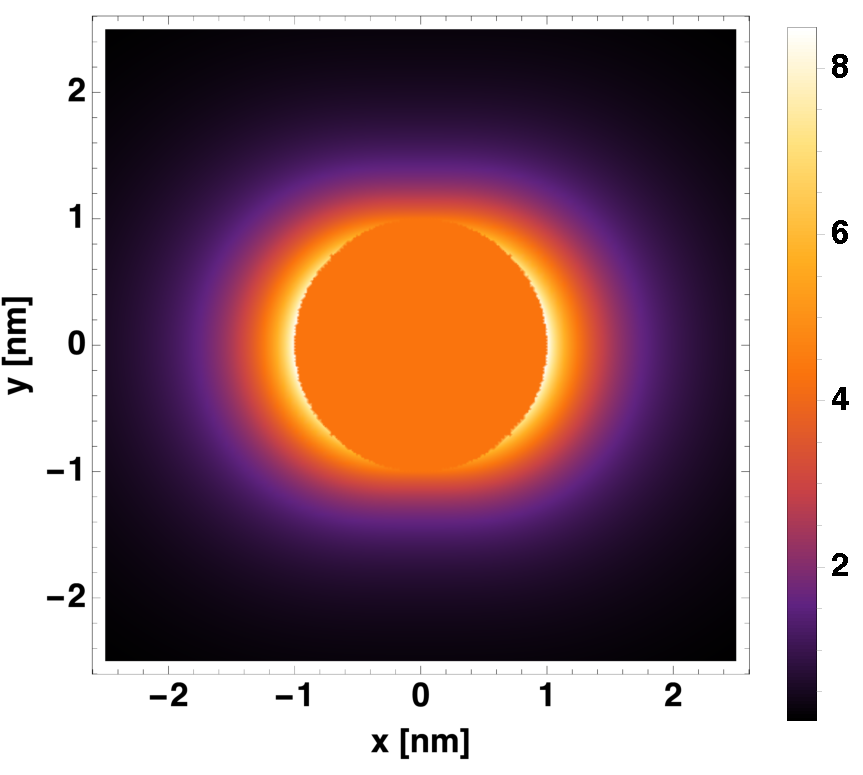
\includegraphics[width=170pt]{ME1.pdf}
\caption{}
\end{subfigure}
\begin{subfigure}[c]{0.5\textwidth}
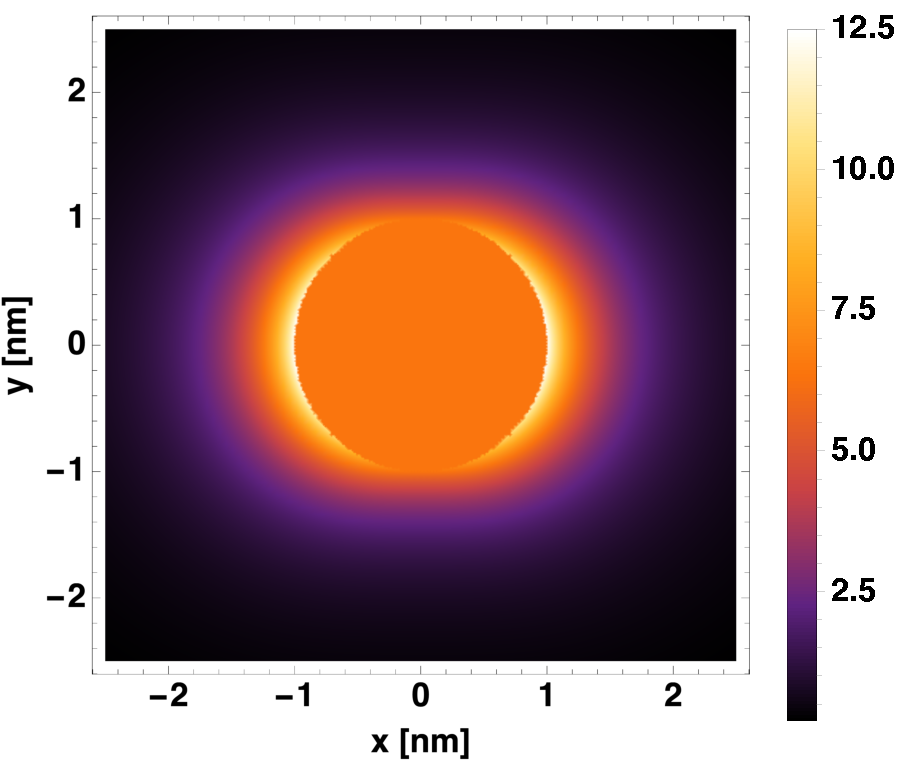
\includegraphics[width=170pt]{ME1(Mar).pdf}
\caption{}
\end{subfigure}
\begin{subfigure}[c]{0.5\textwidth}
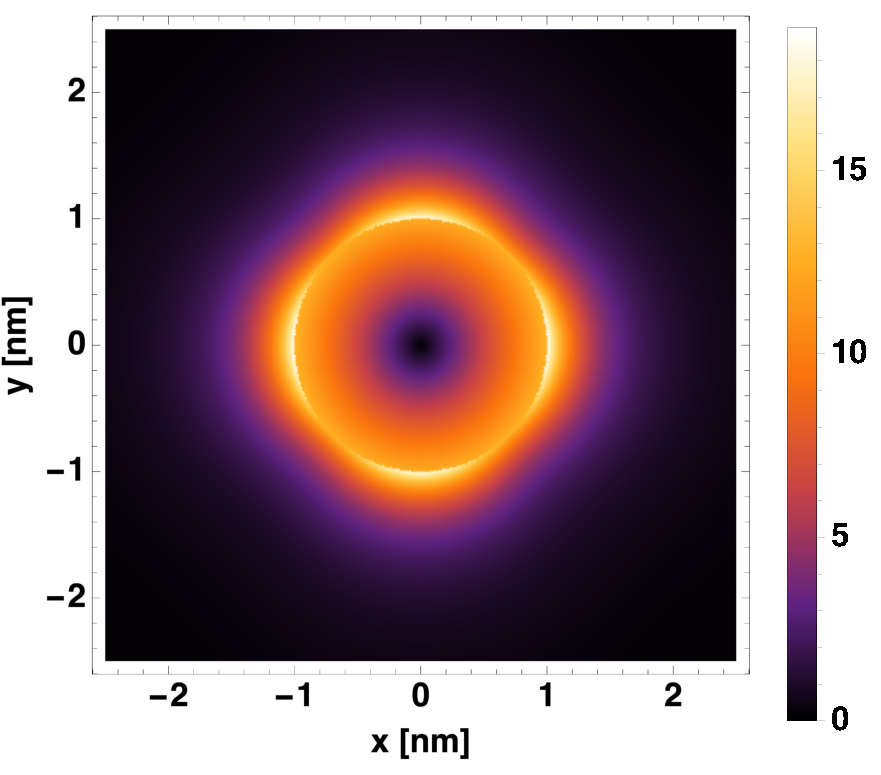
\includegraphics[width=170pt]{ME2.pdf}
\caption{}
\end{subfigure}
\begin{subfigure}[c]{0.5\textwidth}
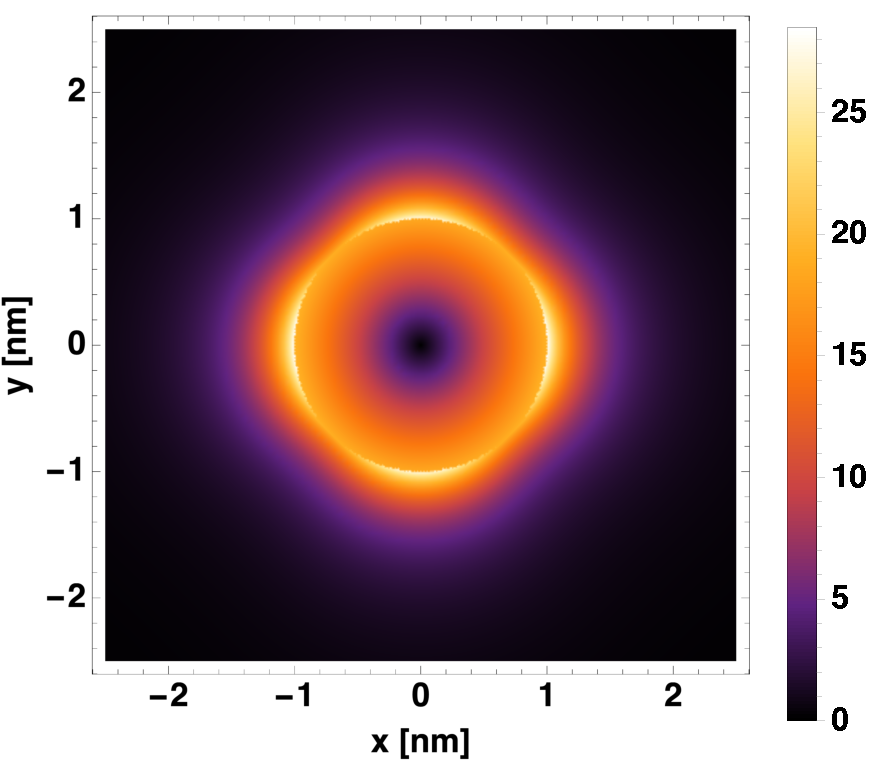
\includegraphics[width=170pt]{ME2(Mar).pdf}
\caption{}
\end{subfigure}
\begin{subfigure}[c]{0.5\textwidth}
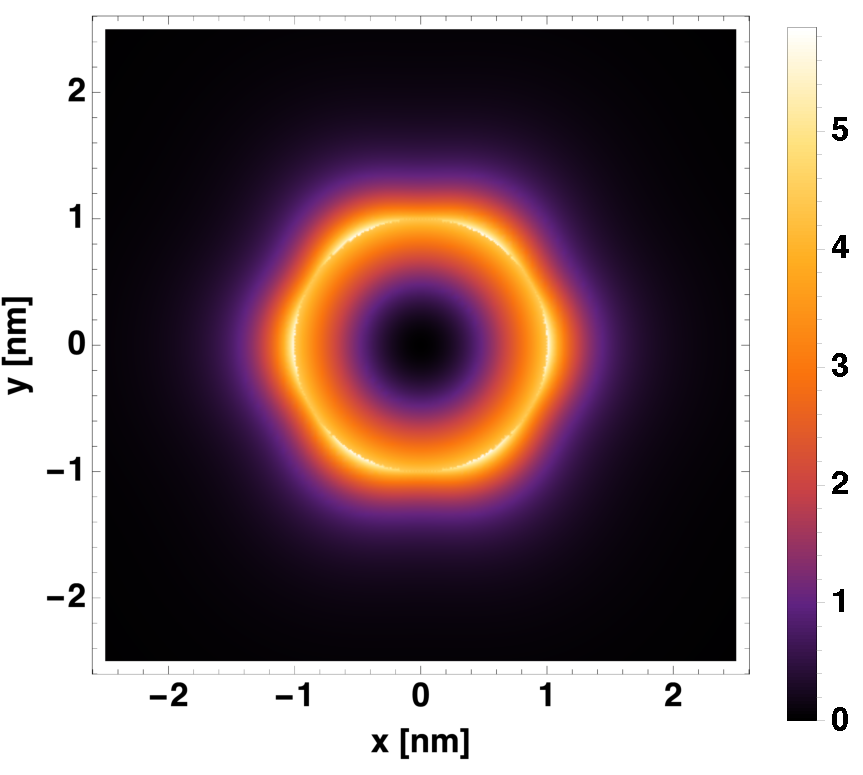
\includegraphics[width=170pt]{ME3.pdf}
\caption{}
\end{subfigure}
\begin{subfigure}[c]{0.5\textwidth}
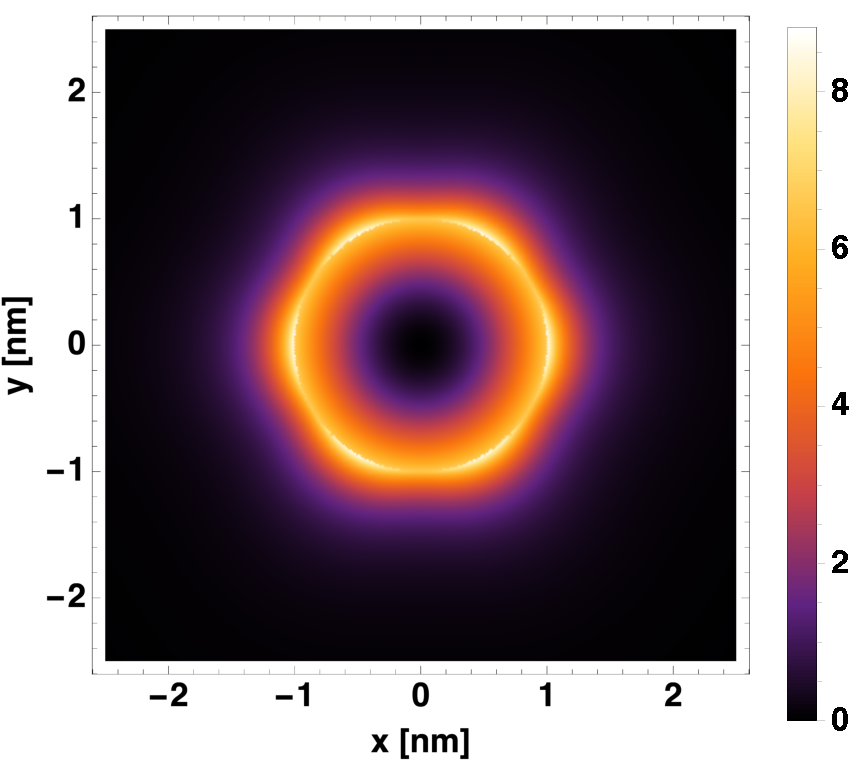
\includegraphics[width=170pt]{ME3(Mar).pdf}
\caption{}
\end{subfigure}
\begin{subfigure}[c]{0.5\textwidth}
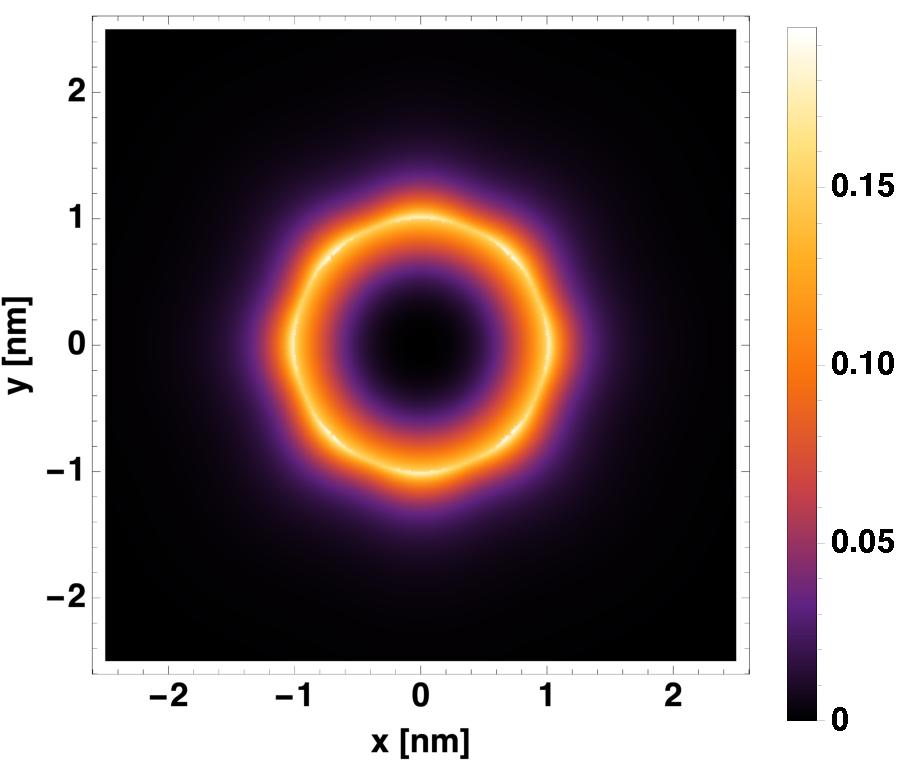
\includegraphics[width=170pt]{ME4.pdf}
\caption{}
\end{subfigure}
\begin{subfigure}[c]{0.5\textwidth}
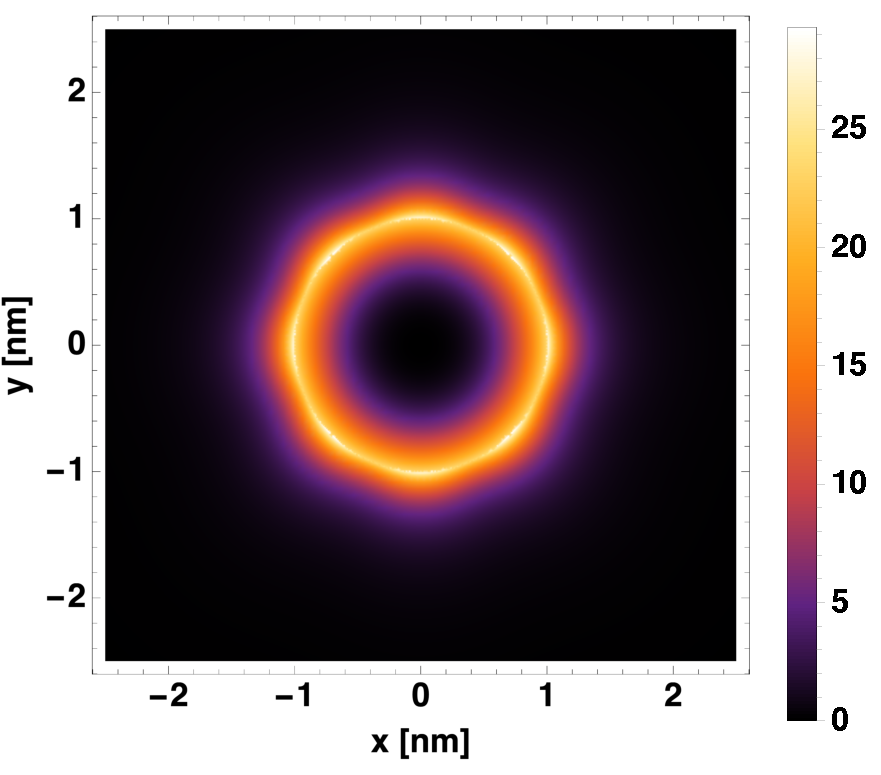
\includegraphics[width=180pt]{ME4(Mar).pdf}
\caption{}
\end{subfigure}
\caption{Gráficas de la magnitud del campo eléctrico inducido en una nanopartícula de aluminio modelada con Drude de 1 nm de radio en presencia de un electrón con rapidez $v$=0.5$c$ y parámetro de impacto $b$=1.5 nm en sus distintas contribuciones multipolares. $|\textbf{E}^{ind}|$ con parámetros $\hbar\omega_p$=13.144 eV y $\hbar\Gamma$=0.197 eV para (a) $l$=1 y $\hbar\omega$=7.859 eV, (c) $l$=2 y $\hbar\omega$=8.313 eV, (e) $l$=3 y $\hbar\omega$=8.605 eV, (g) $l$=4 y $\hbar\omega$=8.762 eV.} 
\end{figure}

\begin{figure}[htb!]
\begin{subfigure}[b]{0.5\textwidth}
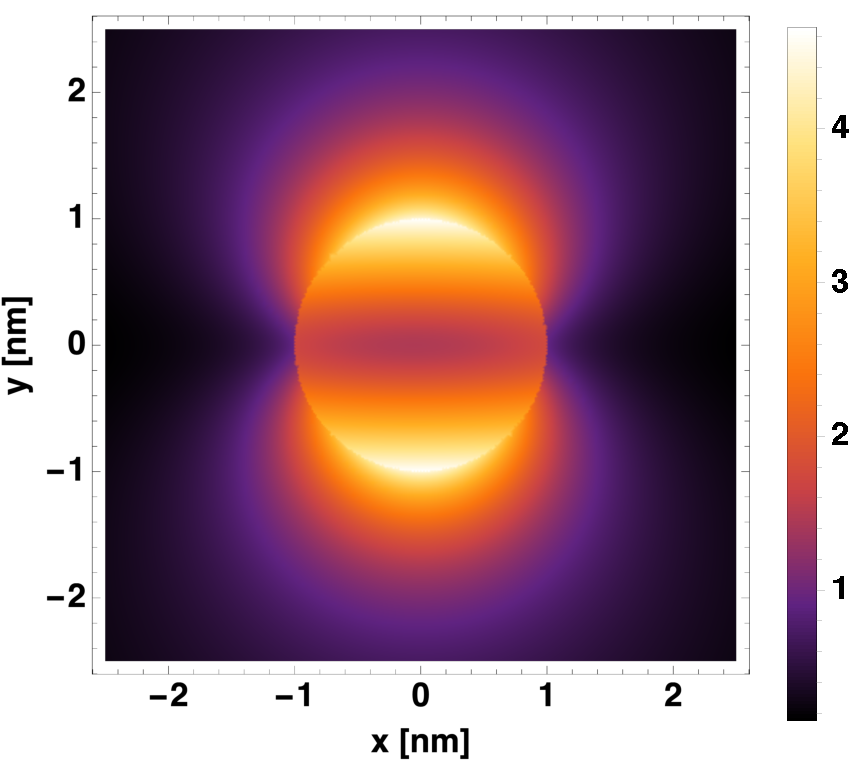
\includegraphics[width=180pt]{MH1.pdf}
\caption{}
\end{subfigure}
\begin{subfigure}[b]{0.5\textwidth}
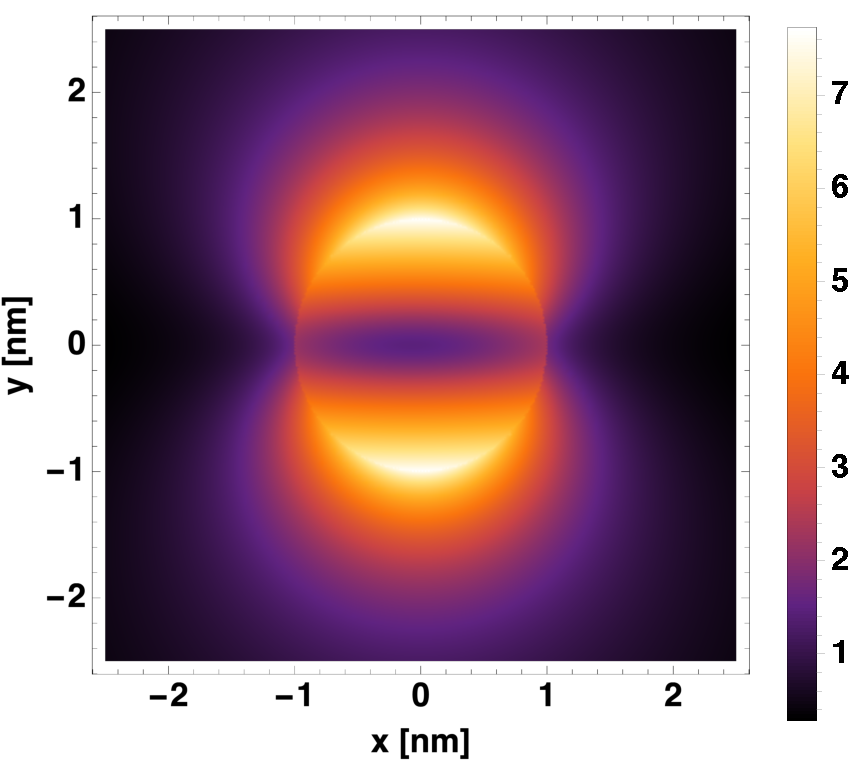
\includegraphics[width=180pt]{MH1(Mar).pdf}
\caption{}
\end{subfigure}
\begin{subfigure}[b]{0.5\textwidth}
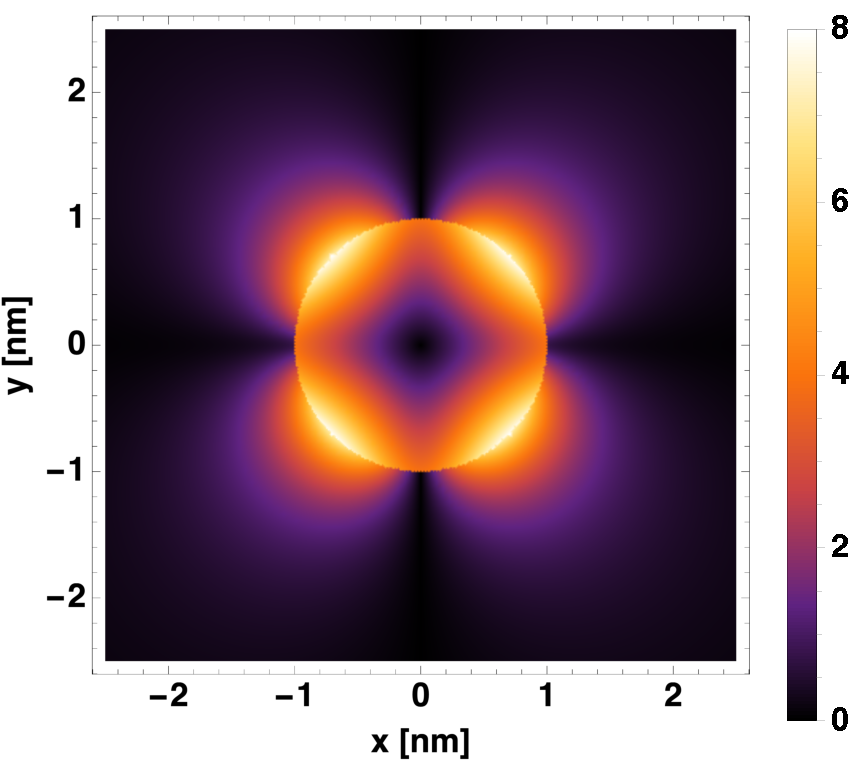
\includegraphics[width=180pt]{MH2.pdf}
\caption{}
\end{subfigure}
\begin{subfigure}[b]{0.5\textwidth}
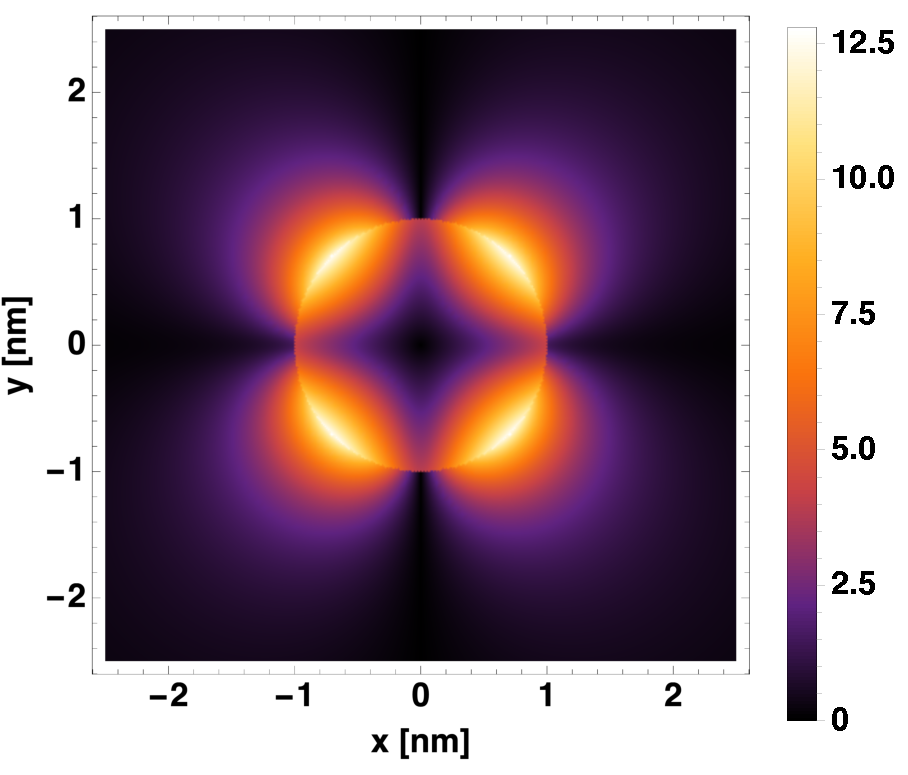
\includegraphics[width=180pt]{MH2(Mar).pdf}
\caption{}
\end{subfigure}
\begin{subfigure}[b]{0.5\textwidth}
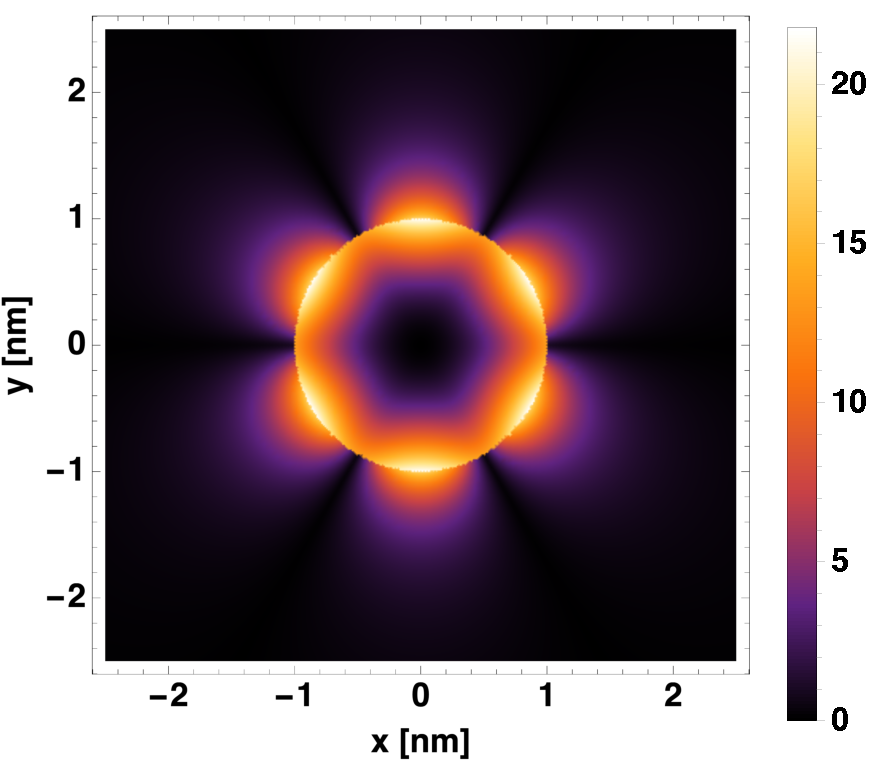
\includegraphics[width=180pt]{MH3.pdf}
\caption{}
\end{subfigure}
\begin{subfigure}[b]{0.5\textwidth}
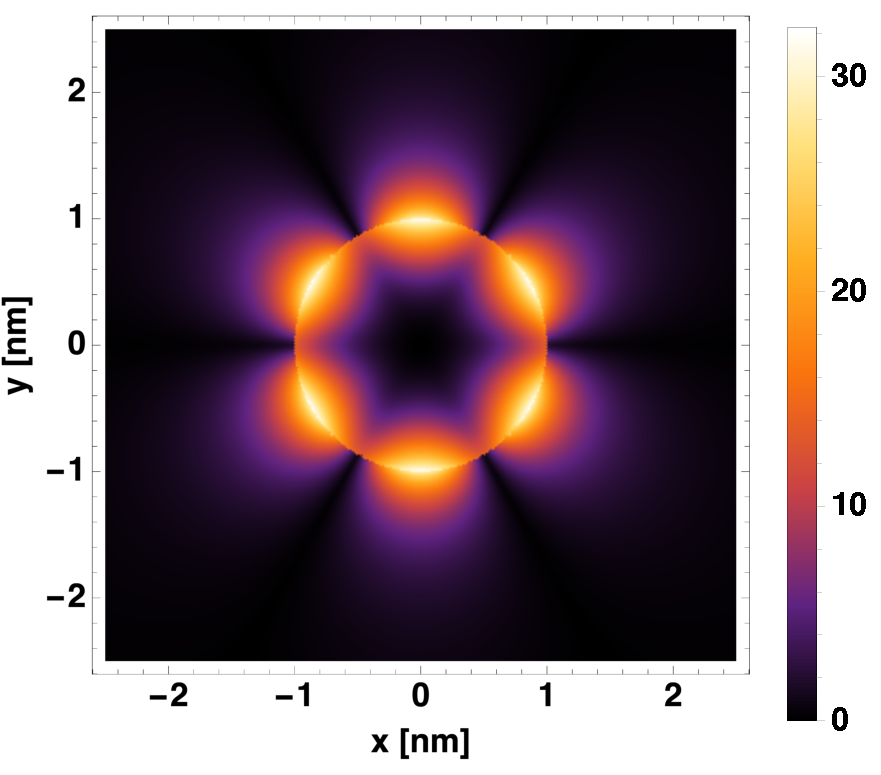
\includegraphics[width=180pt]{MH3(Mar).pdf}
\caption{}
\end{subfigure}
\begin{subfigure}[b]{0.5\textwidth}
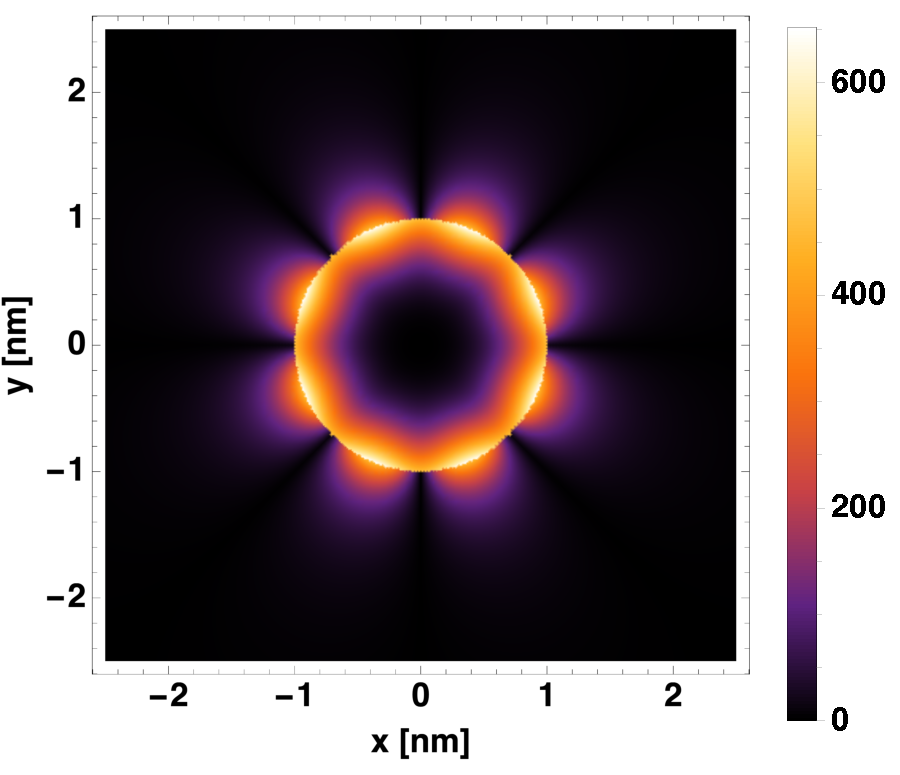
\includegraphics[width=180pt]{MH4.pdf}
\caption{}
\end{subfigure}
\begin{subfigure}[b]{0.5\textwidth}
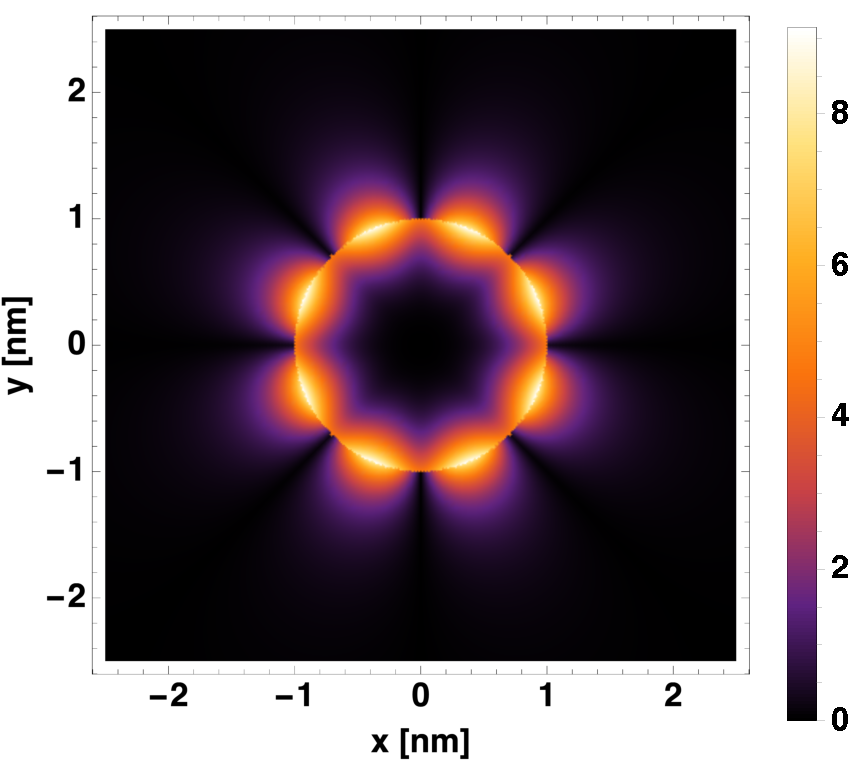
\includegraphics[width=180pt]{MH4(Mar).pdf}
\caption{}
\end{subfigure}
\caption{Magnitud de la contribución multipolar de orden }
\end{figure}

\begin{figure}[htb!]
\begin{subfigure}[b]{0.5\textwidth}
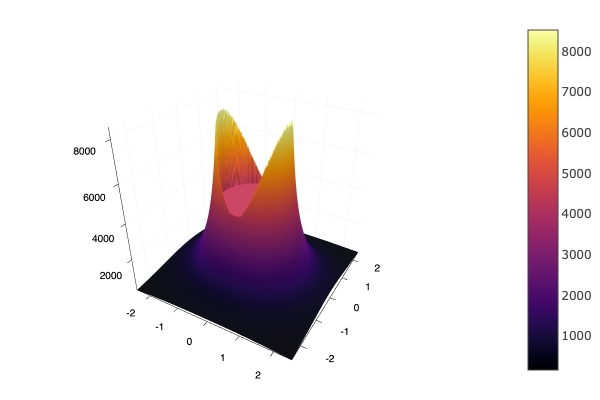
\includegraphics[width=220pt]{E1julia.png}
\caption{}
\label{fig:westminster_lateral}
\end{subfigure}
\begin{subfigure}[b]{0.5\textwidth}
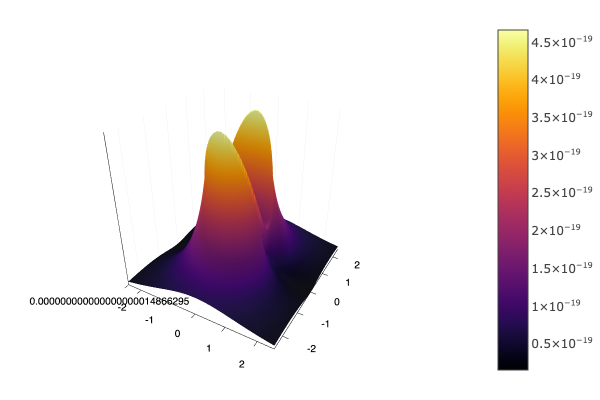
\includegraphics[width=220pt]{H1julia.png}
\caption{}
\end{subfigure}
\begin{subfigure}[b]{0.5\textwidth}
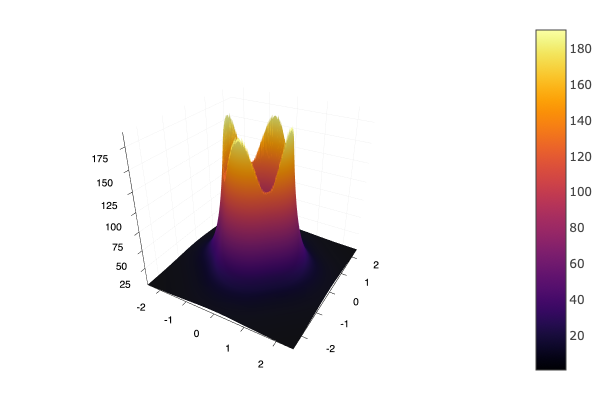
\includegraphics[width=220pt]{E2julia.png}
\caption{}
\end{subfigure}
\begin{subfigure}[b]{0.5\textwidth}
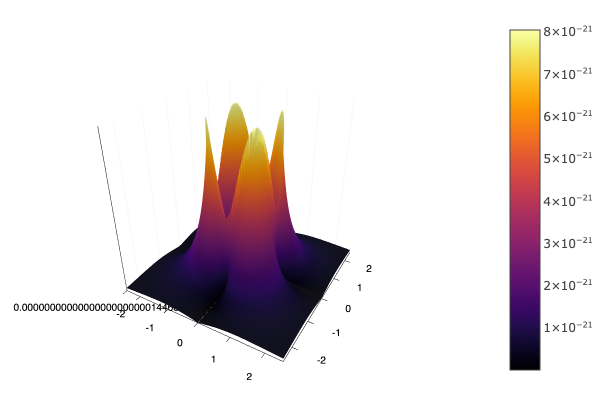
\includegraphics[width=220pt]{H2julia.png}
\caption{}
\end{subfigure}
\begin{subfigure}[b]{0.5\textwidth}
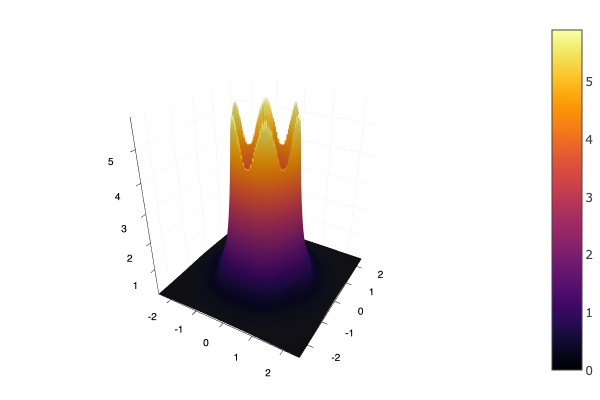
\includegraphics[width=220pt]{E3julia.png}
\caption{}
\end{subfigure}
\begin{subfigure}[b]{0.5\textwidth}
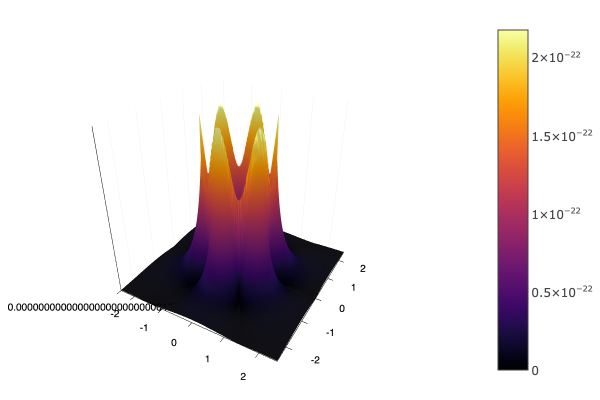
\includegraphics[width=220pt]{H3julia.png}
\caption{}
\end{subfigure}
\begin{subfigure}[b]{0.5\textwidth}
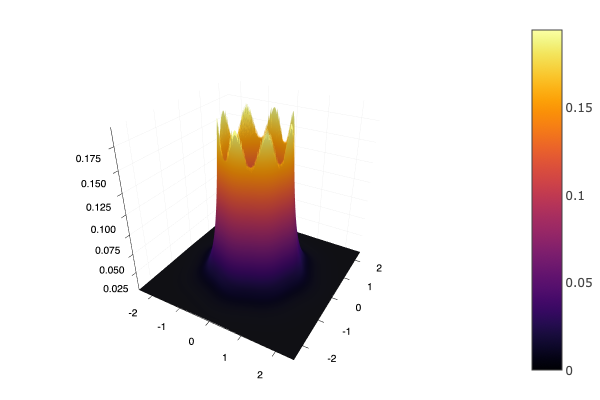
\includegraphics[width=220pt]{E4julia.png}
\caption{}
\end{subfigure}
\begin{subfigure}[b]{0.5\textwidth}
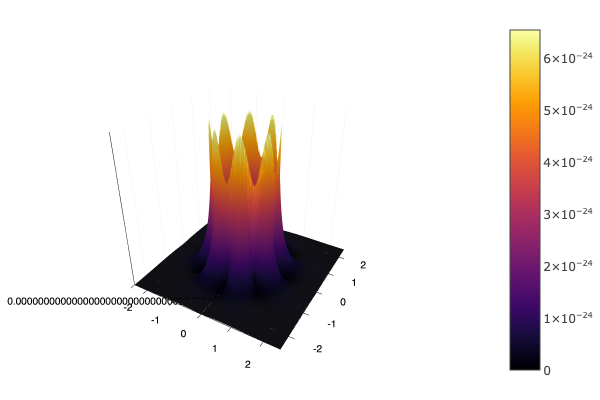
\includegraphics[width=220pt]{H4julia.png}
\caption{}
\end{subfigure}
\caption{Gráficas de la magnitud de los campos electromagnéticos inducidos en una nanopartícula de aluminio modelada con Drude ($\hbar\omega_p$=13.144 eV y $\hbar\Gamma$=0.197 eV ) de 1 nm de radio en presencia de un electrón con rapidez $v$=0.5$c$ y parámetro de impacto $b$=1.5 nm en sus distintas contribuciones multipolares. (a) $|\textbf{E}^{ind}|$ y (b) $|\textbf{H}^{ind}|$ para $l$=1 y $\hbar\omega$=7.589 eV, (c) $|\textbf{E}^{ind}|$ y (d) $|\textbf{H}^{ind}|$ para $l$=2 y $\hbar\omega$=8.313 eV, (e) $|\textbf{E}^{ind}|$ y (f) $|\textbf{H}^{ind}|$ para $l$=3 y $\hbar\omega$=8.605 eV, (g) $|\textbf{E}^{ind}|$ y (h) $|\textbf{H}^{ind}|$ para $l$=4 y $\hbar\omega$=8.762 eV.}
\end{figure}

\section{\large{Cálculo del vector de Poynting del campo EM externo}}

Dado el campo EM externo de las expresiones (1.17) y (1.18), se calcula el vector de Poynting asociado mediante

\begin{equation}
\mathbf{S}^{\text{ext}}(\mathbf{r};t)=\frac{1}{\mu_0}\mathbf{E}^{\text{ext}}(\mathbf{r};t)\times\mathbf{B}^{\text{ext}}(\mathbf{r};t),
\end{equation}

de modo que,

\begin{align}
\mathbf{S}^{\text{ext}}(\mathbf{r};t)
&=\frac{1}{\mu_0}\left(\frac{q\gamma}{4\pi\epsilon_0}\right)\left\{\frac{(x-b)\hatbf{e}_x+y\hatbf{e}_y+(z-vt)\hatbf{e}_z}{[(x-b)^2+y^2+\gamma^2(z-vt)^2]^{3/2}}\right\}\times\left(\frac{\mu_0 q\gamma v}{4\pi}\right)\left\{\frac{-y\hatbf{e}_x+(x-b)\hatbf{e}_y}{[(x-b)^2+y^2+\gamma^2(z-vt)^2]^{3/2}}\right\} \\
&=\left(\frac{q^2\gamma^2 v}{16\pi^2 \epsilon_0}\right)\left\{\frac{[(x-b)\hatbf{e}_x+y\hatbf{e}_y+(z-vt)\hatbf{e}_z]\times[-y\hatbf{e}_x+(x-b)\hatbf{e}_y]}{[(x-b)^2+y^2+\gamma^2(z-vt)^2]^{3/2}}\right\}\\
&=\left(\frac{q^2\gamma^2 v}{16\pi^2 \epsilon_0}\right)\left\{\frac{-(x-b)(z-vt)\hatbf{e}_x-y(z-vt)\hatbf{e}_y+[(x-b)^2+y^2]\hatbf{e}_z]}{[(x-b)^2+y^2+\gamma^2(z-vt)^2]^{3/2}}\right\}
\end{align}

y por componentes

\begin{align}
S^{\text{ext}}_x(\mathbf{r};t)&=-\left(\frac{q^2\gamma^2 v}{16\pi^2 \epsilon_0}\right)\frac{(x-b)(z-vt)}{[(x-b)^2+y^2+\gamma^2(z-vt)^2]^{3/2}}\\
S^{\text{ext}}_y(\mathbf{r};t)&=-\left(\frac{q^2\gamma^2 v}{16\pi^2 \epsilon_0}\right)\frac{y(z-vt)}{[(x-b)^2+y^2+\gamma^2(z-vt)^2]^{3/2}}\\
S^{\text{ext}}_z(\mathbf{r};t)&=\left(\frac{q^2\gamma^2 v}{16\pi^2 \epsilon_0}\right)\frac{(x-b)^2+y^2}{[(x-b)^2+y^2+\gamma^2(z-vt)^2]^{3/2}}
\end{align}


\end{document}